\documentclass[12pt,a4paper,twoside]{report}

\usepackage[utf8]{inputenc}
\usepackage[T1]{fontenc}
\usepackage[polish]{babel}
\usepackage{csquotes}
\usepackage{lmodern}
\usepackage{amssymb}
\usepackage{graphicx}
\usepackage{float}
\usepackage{booktabs}
\usepackage{array}
\newcolumntype{L}[1]{>{\raggedright\arraybackslash}p{#1}}
\usepackage{siunitx}
\sisetup{
    output-decimal-marker={,},
    group-separator={\,},
    group-minimum-digits=4,
    per-mode=symbol,
    detect-all
}
\usepackage{hyperref}
\usepackage{listings}
\usepackage{xcolor}
\usepackage{tikz}
\usetikzlibrary{positioning, arrows.meta, fit}
\usepackage[backend=biber,style=ieee]{biblatex}

\addbibresource{bibliography.bib}

% Pełne polskie formy w bibliografii, niezależnie od wersji biblatex/polish.lbx
% (starsze wersje skracają je do "term. wiz.", "adr.:", "spraw. tech.", "ser.").
\DefineBibliographyStrings{polish}{
    urlseen    = {dostęp},
    url        = {URL},
    techreport = {sprawozdanie techniczne},
}
\graphicspath{{figures/}{logos/}}

\hypersetup{
    pdftitle={Blockchain jako zdecentralizowana infrastruktura klucza publicznego},
    pdfauthor={Adrian Jabłoński}
}

% Konfiguracja listingów kodu
\definecolor{lstkeyword}{rgb}{0.0,0.0,0.6}
\definecolor{lstcomment}{rgb}{0.35,0.45,0.35}
\definecolor{lststring}{rgb}{0.55,0.10,0.10}
\definecolor{lstbg}{rgb}{0.97,0.97,0.97}
\lstset{
    basicstyle=\ttfamily\footnotesize,
    keywordstyle=\color{lstkeyword}\bfseries,
    commentstyle=\color{lstcomment}\itshape,
    stringstyle=\color{lststring},
    backgroundcolor=\color{lstbg},
    numbers=left,
    numberstyle=\tiny\color{gray},
    numbersep=8pt,
    frame=single,
    rulecolor=\color{gray!40},
    breaklines=true,
    showstringspaces=false,
    tabsize=4,
    captionpos=b,
    literate={ą}{{\k{a}}}1 {ę}{{\k{e}}}1 {ó}{{\'o}}1 {ł}{{\l{}}}1
             {ż}{{\.z}}1 {ź}{{\'z}}1 {ć}{{\'c}}1 {ś}{{\'s}}1 {ń}{{\'n}}1
}
\lstdefinelanguage{protobuf}{
    keywords={message,enum,oneof,repeated,optional,reserved,syntax,package,option,import,string,bytes,bool,int64,uint64,int32,uint32},
    morecomment=[l]{//},
    morestring=[b]",
    sensitive=true,
}

\emergencystretch=3em

\title{Blockchain jako zdecentralizowana infrastruktura klucza publicznego}
\author{Adrian Jabłoński}

\begin{document}

\begin{titlepage}
    \thispagestyle{empty}
    \sffamily
    \begin{center}

        \noindent
        \begin{minipage}[c]{0.15\textwidth}
            
\includegraphics[height=2.2cm]{logoPK.jpg}
        \end{minipage}\hfill
        \begin{minipage}[c]{0.66\textwidth}
            \centering
            {\fontsize{16}{19}\selectfont\bfseries Politechnika Krakowska\\[0.15cm]
                im. Tadeusza Kościuszki}\\[0.25cm]
            {\fontsize{16}{19}\selectfont Wydział Informatyki i Matematyki}
        \end{minipage}\hfill
        \begin{minipage}[c]{0.15\textwidth}
            \raggedleft
            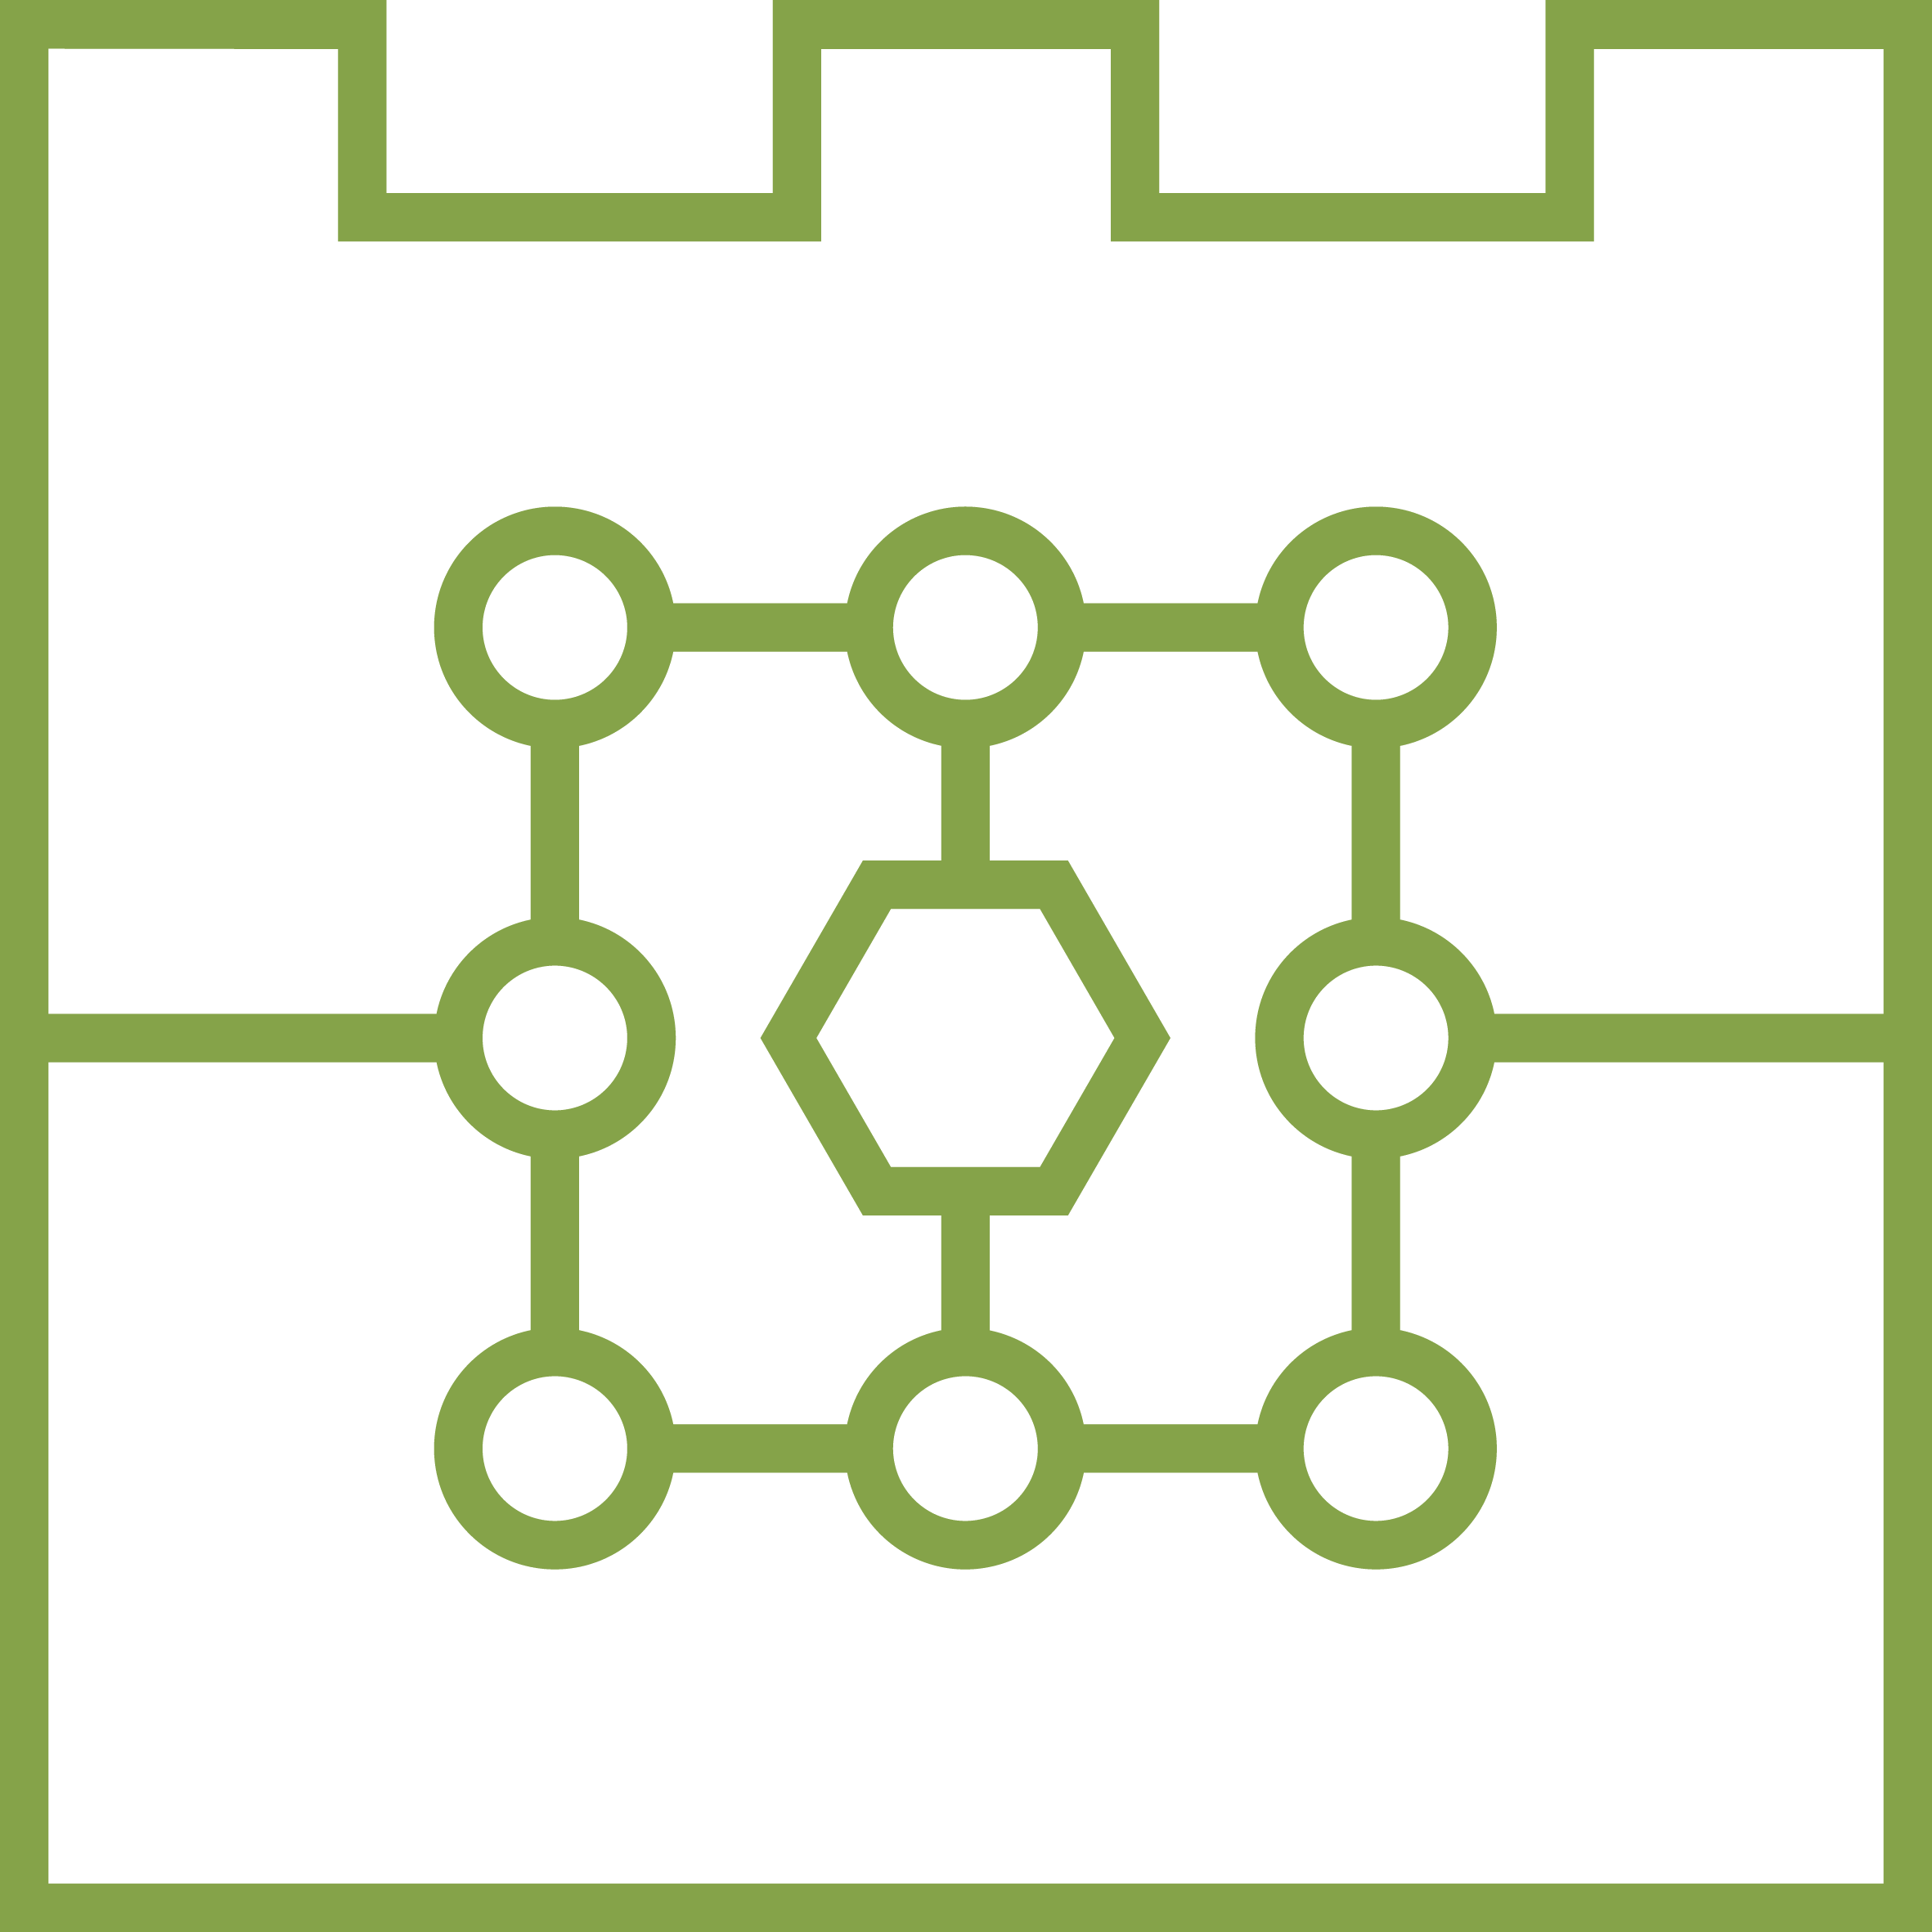
\includegraphics[height=2.2cm]{logoWIIT.png}
        \end{minipage}

        \vspace{3.6cm}

        {\fontsize{14}{17}\selectfont\bfseries Adrian Jabłoński}\\[0.3cm]
        {\fontsize{12}{14}\selectfont Numer albumu: 156764}

        \vspace{1.6cm}

        {\fontsize{16}{19}\selectfont\bfseries Blockchain jako zdecentralizowana infrastruktura klucza publicznego~--- projektowanie, implementacja i analiza bezpieczeństwa}

        \vspace{1.2cm}

        {\fontsize{16}{19}\selectfont\bfseries Blockchain as a decentralized public key infrastructure~--- design, implementation and security analysis}

        \vspace{1.1cm}

        {\fontsize{14}{17}\selectfont\bfseries Praca magisterska na kierunku INFORMATYKA\\[0.2cm]
            specjalność CYBERBEZPIECZEŃSTWO}

        \vspace{2.4cm}

        \begin{flushright}
            {\fontsize{12}{14}\selectfont\bfseries Praca wykonana pod kierunkiem:\\
                dr Agnieszka Jakóbik}
        \end{flushright}

        \vfill

        {\fontsize{12}{14}\selectfont\bfseries Kraków, 2026}

    \end{center}
\end{titlepage}


%!TEX root = ../main.tex
\chapter*{Streszczenie}
\addcontentsline{toc}{chapter}{Streszczenie}

Infrastruktura klucza publicznego (PKI) w obecnym kształcie, opartym na standardzie X.509 i hierarchii urzędów certyfikacji (CA), cierpi na strukturalną słabość: każdy z setek zaufanych urzędów może wystawić ważny certyfikat dla dowolnej domeny, przez co bezpieczeństwo całego systemu wyznacza najsłabsze ogniwo, a mechanizmy unieważniania (CRL, OCSP) pozostają scentralizowane i zawodne. Niniejsza praca podejmuje problem, w jakim stopniu zdecentralizowana infrastruktura klucza publicznego (DPKI) oparta na technologii blockchain może wyeliminować tę słabość w kontekście Web PKI.

Celem pracy było zaprojektowanie, implementacja oraz analiza bezpieczeństwa systemu DPKI stanowiącego alternatywę dla modelu scentralizowanego. Zaprojektowany system jest rejestrem wiązań nazwy domeny z kluczem publicznym, utrzymywanym przez sieć walidatorów z konsensusem bizantyjskim (BFT). Prototyp zaimplementowano w języku Go jako aplikację interfejsu ABCI nad gotowym silnikiem konsensusu CometBFT; stan rejestru przechowywany jest w rzadkim drzewie Merkle, umożliwiającym zwięzłe dowody istnienia i nieistnienia wiązań, a kontrolę nad domeną weryfikuje się metodą wyzwania DNS-01. Analizę bezpieczeństwa przeprowadzono metodą STRIDE, a właściwości wydajnościowe zmierzono na uruchomionej sieci wielowęzłowej.

Wyniki potwierdziły postawione tezy. System eliminuje pojedynczy punkt zaufania, ponieważ kompromitacja mniejszości walidatorów nie narusza integralności rejestru. Unieważnienia propagują się w czasie rzędu jednej sekundy, deterministycznie i z dowodem kryptograficznym, a rozmiar dowodu rośnie jedynie logarytmicznie z liczbą domen. Wykazano zarazem ograniczenia podejścia, w tym zależność od bezpieczeństwa DNS w chwili rejestracji oraz koszt replikacji stanu.

\vspace{1em}
\noindent\textbf{Słowa kluczowe:} blockchain, infrastruktura klucza publicznego, PKI, DPKI, kryptografia asymetryczna, rozproszony rejestr, CometBFT, bezpieczeństwo systemów rozproszonych
%!TEX root = ../main.tex
\chapter*{Abstract}
\addcontentsline{toc}{chapter}{Abstract}

\selectlanguage{english}

Public key infrastructure (PKI) in its current form, based on the X.509 standard and a hierarchy of certificate authorities (CAs), suffers from a structural weakness: any one of the hundreds of trusted authorities can issue a valid certificate for any domain, so the security of the whole system is bounded by its weakest link, while revocation mechanisms (CRL, OCSP) remain centralized and unreliable. This thesis addresses the question of to what extent a decentralized public key infrastructure (DPKI) based on blockchain technology can eliminate this weakness in the context of Web PKI.

The aim of the work was to design, implement, and analyse the security of a DPKI system as an alternative to the centralized model. The proposed system is a registry of bindings between a domain name and a public key, maintained by a network of validators running Byzantine fault-tolerant (BFT) consensus. The prototype was implemented in Go as an ABCI application on top of the existing CometBFT consensus engine; the registry state is stored in a Sparse Merkle Tree, enabling compact proofs of both inclusion and non-inclusion of bindings, and control over a domain is verified using a DNS-01 challenge. The security analysis was conducted with the STRIDE methodology, and performance properties were measured on a running multi-node network.

The results confirmed the stated theses: the system eliminates the single point of trust -- compromising a minority of validators does not violate registry integrity -- propagates revocations within about one second, deterministically and with a cryptographic proof, while proof size grows only logarithmically with the number of domains. The limitations of the approach were also demonstrated, including the dependence on DNS security at registration time and the cost of state replication.

\vspace{1em}
\noindent\textbf{Keywords:} blockchain, public key infrastructure, PKI, DPKI, asymmetric cryptography, distributed ledger, CometBFT, distributed systems security

\selectlanguage{polish}

\tableofcontents

%!TEX root = ../main.tex
\chapter*{Wykaz skrótów i akronimów}
\addcontentsline{toc}{chapter}{Wykaz skrótów i akronimów}

\begin{description}
    \item[ABCI] Application Blockchain Interface
    \item[ACME] Automatic Certificate Management Environment
    \item[API] Application Programming Interface
    \item[BFT] Byzantine Fault Tolerance
    \item[CA] Certificate Authority
    \item[CRL] Certificate Revocation List
    \item[CT] Certificate Transparency
    \item[DNS] Domain Name System
    \item[DPKI] Decentralized Public Key Infrastructure
    \item[OCSP] Online Certificate Status Protocol
    \item[P2P] Peer-to-Peer
    \item[PKI] Public Key Infrastructure
    \item[RPC] Remote Procedure Call
    \item[SMT] Sparse Merkle Tree
    \item[SSI] Self-Sovereign Identity
    \item[TLS] Transport Layer Security
\end{description}

\chapter{Wstęp}
\label{ch:wstep}

\section{Motywacja}
\label{sec:motywacja}

Infrastruktura klucza publicznego (PKI) jest fundamentem zaufania w Internecie. Odpowiada za uwierzytelnianie stron komunikacji w protokole TLS, podpisywanie kodu, zabezpieczanie poczty elektronicznej oraz wiele innych zastosowań kryptograficznych. W obecnym kształcie, opartym na standardzie X.509, model zaufania PKI ma charakter hierarchiczny i wymaga obecności zaufanych centrów certyfikacji (CA), które poświadczają powiązanie tożsamości z kluczem publicznym.

Ta hierarchiczna konstrukcja niesie ze sobą szereg problemów strukturalnych. Każde z setek centrów certyfikacji obecnych w globalnych magazynach zaufania (\emph{trust stores}) przeglądarek i systemów operacyjnych \cite{mozilla-ca-list} może wystawić ważny certyfikat dla dowolnej domeny w Internecie, co oznacza, że bezpieczeństwo całego systemu jest ograniczone bezpieczeństwem najsłabszego z CA. Historia PKI dostarcza konkretnych przykładów konsekwencji tego stanu rzeczy. Włamanie do holenderskiego CA DigiNotar w 2011 roku skutkowało wystawieniem ponad pięciuset fałszywych certyfikatów, w tym dla domeny \texttt{*.google.com}, wykorzystywanych do masowej inwigilacji obywateli Iranu \cite{foxit-blacktulip}. Kilkukrotne nieprawidłowości w wystawianiu certyfikatów przez Symantec doprowadziły z kolei do usunięcia tego CA z magazynów zaufania głównych przeglądarek w latach 2017--2018 \cite{google-symantec-distrust}. Także scentralizowany charakter mechanizmów unieważniania certyfikatów (CRL, OCSP) generuje problemy z wydajnością, prywatnością i dostępnością, które do dziś nie doczekały się satysfakcjonującego rozwiązania.

Częściową odpowiedzią na te problemy jest Certificate Transparency (CT) \cite{rfc6962}, czyli mechanizm publicznych, niezmienialnych logów certyfikatów, do których wszystkie wystawione przez CA certyfikaty muszą zostać dopisane, by przeglądarki uznały je za ważne. CT zwiększa wykrywalność nadużyć, ale nie eliminuje samego problemu, ponieważ nadal opiera się na zaufaniu do operatorów logów oraz CA i pełni rolę detekcyjną, a nie prewencyjną.

Technologia blockchain, zaproponowana w 2008 roku w kontekście kryptowaluty Bitcoin \cite{nakamoto2008bitcoin}, oferuje właściwości, które potencjalnie mogą zaadresować strukturalne słabości klasycznej PKI: rozproszony konsensus, niezmienność historii, transparentność oraz brak pojedynczego punktu zaufania. Koncepcja zdecentralizowanej infrastruktury klucza publicznego (DPKI) \cite{allen2015dpki} zakłada, że wiązanie tożsamości z kluczem publicznym może zostać zapisane w rozproszonym rejestrze utrzymywanym wspólnie przez wiele niezależnych podmiotów, eliminując konieczność istnienia zaufanego pośrednika.

Mimo licznych prób implementacji tej koncepcji, od Namecoina \cite{kalodner2015namecoin}, przez Blockstack \cite{ali2016blockstack}, po systemy oparte na tożsamości suwerennej (SSI) \cite{w3c-did-core}, żadne z istniejących rozwiązań nie zyskało powszechnego uznania w roli zamiennika klasycznej PKI. Otwartymi problemami pozostają inicjalizacja zaufania w nowo uruchamianej sieci, wydajność, koszt operacji oraz integracja z istniejącymi standardami i narzędziami. Tematyka ta pozostaje aktywnym obszarem badań akademickich i przemysłowych, a kompleksowe podejście łączące projektowanie, implementację oraz analizę bezpieczeństwa systemu DPKI stanowi wartościowy wkład w dyskusję nad kierunkami ewolucji PKI.

\section{Cel i zakres pracy}
\label{sec:cel-zakres}

Głównym celem pracy jest zaprojektowanie, implementacja oraz analiza bezpieczeństwa zdecentralizowanej infrastruktury klucza publicznego opartej na technologii blockchain, stanowiącej alternatywę dla scentralizowanego modelu PKI X.509 w przypadku użycia Web PKI, czyli wiązania nazw domen z kluczami publicznymi na potrzeby uwierzytelniania w protokole TLS.

Zakres pracy obejmuje analizę porównawczą klasycznej PKI X.509 oraz istniejących podejść zdecentralizowanych, przegląd platform blockchain pod kątem przydatności do roli rozproszonego rejestru certyfikatów, zaprojektowanie architektury systemu wraz z modelem danych i protokołami operacji na certyfikatach (rejestracja, weryfikacja, odnowienie, unieważnienie), implementację prototypu w języku Go obejmującą warstwę aplikacyjną blockchain oraz aplikację kliencką, a także modelowanie zagrożeń i analizę bezpieczeństwa zaproponowanego rozwiązania w odniesieniu do typowych wektorów ataku na PKI. Praca zamyka się porównaniem zaproponowanego systemu z klasyczną PKI pod kątem właściwości bezpieczeństwa, kosztu operacji oraz ograniczeń podejścia.

Jako warstwę konsensusu wybrano CometBFT \cite{cometbft-docs}, kontynuację projektu Tendermint Core \cite{buchman2018tendermint}. Jest to gotowa, przetestowana implementacja algorytmu konsensusu BFT, pozwalająca skupić nakład pracy na warstwie aplikacyjnej, w której znajduje się zasadnicza logika DPKI istotna z punktu widzenia tematu pracy. Komunikacja z warstwą konsensusu odbywa się poprzez interfejs ABCI, a sama logika aplikacji oraz klient zostały zaimplementowane w języku Go.

Otrzymany prototyp nie jest gotowym produktem przeznaczonym do wdrożenia produkcyjnego. Jego celem jest weryfikacja stawianych tez oraz dostarczenie konkretnej, działającej implementacji, na podstawie której można przeprowadzić analizę bezpieczeństwa odnoszącą się do rzeczywistego systemu, a nie wyłącznie do modelu abstrakcyjnego.

\section{Problem badawczy i pytania badawcze}
\label{sec:problem-badawczy}

Problem badawczy podjęty w niniejszej pracy można sformułować następująco: \emph{w jakim stopniu zdecentralizowana infrastruktura klucza publicznego oparta na blockchain jest w stanie wyeliminować strukturalne słabości klasycznego modelu PKI X.509 w kontekście Web PKI, jakie nowe wektory ataku oraz ograniczenia wprowadza takie podejście, oraz czy jego implementacja jest praktycznie wykonalna z wykorzystaniem istniejących komponentów}.

W ramach tak zdefiniowanego problemu sformułowano następujące pytania szczegółowe:
\begin{enumerate}
    \item Które klasy ataków typowe dla scentralizowanej PKI, w szczególności kompromitacja CA, wystawianie nieautoryzowanych certyfikatów oraz opóźnienia w propagacji unieważnień, zostają wyeliminowane przez zastosowanie blockchain jako rejestru, a które pozostają aktualne lub przyjmują nową postać?
    \item Jakie nowe powierzchnie ataku pojawiają się wraz z wprowadzeniem warstwy konsensusu rozproszonego, sieci P2P oraz protokołów rejestracji opartych na wyzwaniach (\emph{challenge-response}), i jak ich istotność wypada w porównaniu z klasami ataków eliminowanymi przez zastosowanie blockchain?
    \item W jaki sposób można zaprojektować mechanizm wiązania domeny z kluczem publicznym, który nie wymaga istnienia zaufanego pośrednika, a jednocześnie pozostaje odporny na próby przejęcia tożsamości?
    \item Czy implementacja funkcjonalnej DPKI jest praktycznie wykonalna z wykorzystaniem gotowych komponentów warstwy konsensusu, bez konieczności implementowania własnego protokołu od podstaw?
\end{enumerate}

\section{Postawione tezy}
\label{sec:tezy}

W pracy postawiono tezę główną oraz cztery tezy pomocnicze, stanowiące przewidywane odpowiedzi na sformułowane wyżej pytania badawcze.

\textbf{Teza główna} stwierdza, że zdecentralizowana infrastruktura klucza publicznego oparta na blockchain z konsensusem BFT może stanowić funkcjonalnie kompletną alternatywę dla klasycznego modelu PKI X.509 w zakresie Web PKI, eliminując pojedynczy punkt zaufania w postaci centrów certyfikacji.

Tezy pomocnicze są następujące:
\begin{enumerate}
    \item Zastąpienie hierarchii zaufanych CA rozproszonym rejestrem opartym na blockchain znacząco ogranicza skuteczność ataków polegających na kompromitacji pojedynczego podmiotu i wystawieniu fałszywego certyfikatu dla cudzej domeny, ponieważ nieautoryzowana zmiana wiązania wymaga kontroli nad znaczącą częścią walidatorów sieci, a nie nad jednym urzędem. Część zagrożeń, związanych z bezpieczeństwem klucza prywatnego właściciela domeny oraz integralnością procesu weryfikacji, pozostaje przy tym aktualna i wymaga niezależnego adresowania.
    \item Wprowadzenie warstwy konsensusu rozproszonego oraz sieci P2P powoduje pojawienie się nowych wektorów ataku, jednak ich realizacja wymaga skompromitowania większościowej części walidatorów lub aktywnego uczestnictwa w protokole sieciowym, co czyni je istotnie trudniejszymi w wykorzystaniu niż kompromitacja pojedynczego CA w modelu klasycznym.
    \item Zapis stanu certyfikatów w blockchainie z wykorzystaniem drzew Merkle umożliwia zaprojektowanie protokołu wiązania domeny z kluczem publicznym pozbawionego zaufanego pośrednika, a weryfikacja istnienia, ważności oraz unieważnienia certyfikatu odbywa się z gwarancjami kryptograficznymi silniejszymi niż mechanizmy CRL i OCSP, przy zachowaniu porównywalnego lub niższego kosztu po stronie weryfikującego.
    \item Wykorzystanie gotowej warstwy konsensusu (CometBFT) oraz interfejsu ABCI pozwala na implementację funkcjonalnej DPKI wyłącznie w warstwie aplikacyjnej, bez konieczności implementowania własnego protokołu konsensusu.
\end{enumerate}

\section{Oryginalny wkład pracy}
\label{sec:wklad}

Poniżej wymieniono to, co w pracy jest wkładem własnym, a nie materiałem zaczerpniętym z literatury ani gotowym komponentem.

\begin{enumerate}
    \item \textbf{Przegląd i porównanie istniejących systemów DPKI.} Analiza Namecoina, Blockstacka, CertCoina, IKP oraz CONIKS. Z porównania wyprowadzono wymagania postawione projektowanemu systemowi (sekcja~\ref{sec:przeglad-rozwiazan}).

    \item \textbf{Projekt systemu.} Architektura trzech warstw, model danych wiązania domena--klucz oraz protokoły czterech operacji: rejestracji, rotacji klucza, unieważnienia i weryfikacji z dowodem (rozdział~\ref{ch:projekt}).

    \item \textbf{Nieodwracalne unieważnienie.} Unieważniony wpis zostaje w stanie rejestru i nie da się go przywrócić. Napastnik, który zdobył klucz właściciela, nie cofnie więc unieważnienia, powtarzając pierwotną transakcję rejestracji (sekcja~\ref{subsec:uniewaznienie}).

    \item \textbf{Wyzwanie DNS związane z kluczem.} Kontrolę nad domeną sprawdza się metodą wzorowaną na ACME DNS-01, ale wartość wyzwania liczona jest tu z klucza publicznego nadawcy transakcji (sekcja~\ref{sec:wlasnosc-domeny}).

    \item \textbf{Weryfikacja DNS przed konsensusem, w dwóch miejscach.} Zapytanie DNS daje różne wyniki w zależności od chwili i miejsca odpytania, więc nie może trafić do wykonania bloku. Umieszczono je w bramce \texttt{CheckTx} i powtórzono przy ocenie cudzej propozycji (\texttt{ProcessProposal}). Wykonanie bloku pozostaje przez to deterministyczne (sekcje~\ref{sec:wlasnosc-domeny} i~\ref{subsec:checktx-finalize}).

    \item \textbf{Trzy tryby weryfikacji po stronie klienta.} Weryfikacja wobec jednego węzła, wobec wielu węzłów naraz oraz offline, względem wcześniej pozyskanego korzenia (sekcja~\ref{sec:api}).

    \item \textbf{Implementacja prototypu w języku Go.} Aplikacja ABCI z całą logiką rejestru, własne rzadkie drzewo Merkle z dowodami włączenia i nieobecności, klient wiersza poleceń weryfikujący dowody lokalnie, generator konfiguracji sieci testowej oraz jej wariant kontenerowy (rozdział~\ref{ch:implementacja}). Łącznie około 4,8~tysiąca linii kodu, nie licząc testów i klas wygenerowanych ze schematu Protocol Buffers. Jedyną istotną biblioteką zewnętrzną jest silnik konsensusu CometBFT.

    \item \textbf{Kompresja dowodów mapą bitową.} Dowód w drzewie o 256 poziomach zawierałby 256 skrótów rodzeństwa, czyli 8~kB. Większość z nich to jednak wartości domyślne, które weryfikujący odtworzy sam, więc przesyłane są tylko pozostałe wartości. 32-bajtowa mapa bitowa wskazuje poziomy, na których się one znajdują. Dzięki temu dowód mieści się w tylko 700~bajtach (sekcja~\ref{subsec:implementacja-merkle}).

    \item \textbf{Zestaw testów.} Około 180 testów jednostkowych, integracyjnych, bezpieczeństwa i rozmytych, uzupełnionych o siedem scenariuszy uruchamianych na sieci czterech walidatorów. Dodatkowo atrapy weryfikatora DNS i węzła RPC, pozwalające testować logikę bez sieci (sekcja~\ref{sec:testy}).

    \item \textbf{Model zagrożeń i katalog ataków.} Pięć klas adwersarzy, klasyfikacja STRIDE dla komponentów systemu oraz dwadzieścia dwa przeanalizowane wektory ataku, z czego dziewiętnaście sprawdzono w testach (sekcja~\ref{sec:zalozenia-adwersarz} i rozdział~\ref{ch:analiza-bezpieczenstwa}).

    \item \textbf{Metodyka i wyniki pomiarów.} Własny program pomiarowy, skrypt uruchamiający całą serię pomiarów w powtarzalnych warunkach oraz skrypt rysujący wykresy z zapisanych wyników, przyjęte zasady pomiaru, a także uzyskane charakterystyki przepustowości, opóźnienia zatwierdzenia transakcji, wzrostu rozmiaru stanu rejestru oraz rozmiaru i czasu weryfikacji dowodów (rozdział~\ref{ch:eksperymenty}).

    \item \textbf{Porównanie z klasyczną PKI.} Zestawienie właściwości bezpieczeństwa (sekcja~\ref{sec:porownanie-bezpieczenstwa}) oraz porównanie kosztów operacji (sekcja~\ref{subsec:porownanie-wydajnosc}), odniesione do słabości wskazanych w rozdziale~\ref{ch:pki-klasyczna}.
\end{enumerate}

Wkładem pracy nie są natomiast gotowe elementy, takie jak: silnik konsensusu CometBFT wraz z protokołem Tendermint, prymitywy Ed25519 i SHA-256, sama koncepcja rzadkiego drzewa Merkle, schemat wyzwania DNS-01 z protokołu ACME oraz metoda STRIDE. Każdy z nich opisano w rozdziałach~\ref{ch:pki-klasyczna}--\ref{ch:dpki} ze wskazaniem źródła.

%!TEX root = ../main.tex
\chapter{Klasyczna infrastruktura klucza publicznego}
\label{ch:pki-klasyczna}

\section{Kryptografia asymetryczna i podpisy cyfrowe}
\label{sec:kryptografia-asymetryczna}

Kryptografia asymetryczna (kryptografia klucza publicznego) opiera się na parze matematycznie powiązanych kluczy: kluczu prywatnym, znanym wyłącznie właścicielowi, oraz kluczu publicznym, który może być swobodnie rozpowszechniany. Koncepcję tę zaproponowali Diffie i Hellman w 1976 roku \cite{diffie1976new}, a pierwszą praktyczną realizację stanowił algorytm RSA \cite{rivest1978rsa}. Konstrukcja pary kluczy gwarantuje, że operacji wykonanej jednym kluczem nie da się odwrócić bez znajomości klucza komplementarnego, a wyznaczenie klucza prywatnego na podstawie publicznego jest obliczeniowo niewykonalne.

Z punktu widzenia infrastruktury klucza publicznego najistotniejszym zastosowaniem kryptografii asymetrycznej jest podpis cyfrowy. Podpisujący wyznacza skrót kryptograficzny wiadomości, a następnie przekształca go z użyciem klucza prywatnego; dowolny weryfikujący, dysponując kluczem publicznym, może sprawdzić, że podpis został złożony przez posiadacza klucza prywatnego oraz że wiadomość nie uległa modyfikacji po podpisaniu. Podpis cyfrowy zapewnia zatem jednocześnie integralność danych, uwierzytelnienie ich pochodzenia oraz niezaprzeczalność.

Obok systemów opartych na problemie faktoryzacji (RSA) powszechnie stosowane są systemy oparte na krzywych eliptycznych, oferujące porównywalny poziom bezpieczeństwa przy znacznie krótszych kluczach. Przykładem jest schemat podpisu EdDSA na krzywej Curve25519, znany jako Ed25519 \cite{rfc8032}, charakteryzujący się 32-bajtowymi kluczami publicznymi, 64-bajtowymi podpisami, wysoką wydajnością oraz deterministyczną konstrukcją podpisu eliminującą klasę błędów implementacyjnych związanych z generowaniem liczb losowych. Z tych powodów Ed25519 został wybrany jako domyślny algorytm podpisu w systemie implementowanym w ramach niniejszej pracy (rozdział~\ref{ch:projekt}).

Sama kryptografia asymetryczna nie rozwiązuje jednak problemu, który legł u podstaw PKI: skąd weryfikujący ma wiedzieć, że dany klucz publiczny rzeczywiście należy do podmiotu, z którym zamierza się komunikować? Jeżeli napastnik zdoła podstawić własny klucz publiczny w miejsce klucza ofiary, może przeprowadzić atak pośrednika (\emph{man-in-the-middle}) - deszyfrować i modyfikować komunikację, pozostając niewykrytym, mimo że wszystkie operacje kryptograficzne przebiegają poprawnie. Problem wiązania tożsamości z kluczem publicznym jest więc problemem zaufania, nie kryptografii, i to właśnie jego rozwiązaniu służy infrastruktura klucza publicznego. Sposób, w jaki to wiązanie jest ustanawiane i odwoływane, definiuje model zaufania całego systemu - i stanowi oś porównania pomiędzy klasyczną PKI a podejściem zdecentralizowanym proponowanym w tej pracy.

\section{Standard X.509 i certyfikaty}
\label{sec:x509}

W klasycznej PKI wiązanie tożsamości z kluczem publicznym przyjmuje postać certyfikatu - podpisanego cyfrowo dokumentu, w którym zaufana trzecia strona (urząd certyfikacji, ang. \emph{Certificate Authority}, CA) poświadcza, że dany klucz publiczny należy do wskazanego podmiotu. Dominującym formatem certyfikatów jest X.509 w wersji 3, którego profil dla zastosowań internetowych definiuje RFC~5280 \cite{rfc5280}.

Certyfikat X.509 zawiera w szczególności:
\begin{itemize}
    \item identyfikację podmiotu (\emph{subject}) - w przypadku Web PKI kluczowa jest tu nazwa domeny, przenoszona współcześnie w rozszerzeniu \emph{Subject Alternative Name};
    \item klucz publiczny podmiotu wraz z identyfikatorem algorytmu;
    \item identyfikację wystawcy (\emph{issuer}), czyli CA, które złożyło podpis;
    \item okres ważności (\emph{not before}, \emph{not after});
    \item numer seryjny, unikalny w obrębie wystawcy, wykorzystywany m.in.\ przy unieważnianiu;
    \item rozszerzenia określające dozwolone zastosowania klucza (\emph{key usage}, \emph{extended key usage}), ograniczenia ścieżki certyfikacji oraz adresy usług związanych z certyfikatem (punkty dystrybucji CRL, adres respondera OCSP);
    \item podpis cyfrowy wystawcy obejmujący całość powyższych danych.
\end{itemize}

W kontekście Web PKI certyfikaty dzieli się zwyczajowo według zakresu weryfikacji przeprowadzonej przez CA: od certyfikatów DV (\emph{Domain Validation}), potwierdzających wyłącznie kontrolę nad domeną, przez OV (\emph{Organization Validation}), po EV (\emph{Extended Validation}), wymagające weryfikacji tożsamości prawnej organizacji. W praktyce zdecydowana większość wystawianych obecnie certyfikatów to certyfikaty DV, czego głównym katalizatorem stało się darmowe CA Let's Encrypt oraz protokół ACME \cite{rfc8555}, automatyzujący weryfikację kontroli nad domeną poprzez wyzwania (\emph{challenge-response}) - np.\ publikację zadanej wartości w rekordzie DNS lub pod wskazanym adresem HTTP. Warto odnotować, że dokładnie ta sama idea weryfikacji przez wyzwanie zostanie wykorzystana w projektowanym systemie DPKI (rozdział~\ref{ch:projekt}), z tą różnicą, że weryfikującym nie będzie pojedyncze CA, lecz niezależnie każdy z walidatorów sieci.

\section{Hierarchia zaufania i rola urzędów certyfikacji}
\label{sec:hierarchia-zaufania}

Certyfikat jest tak wiarygodny, jak podmiot, który go podpisał - przesuwa to pytanie o zaufanie z klucza serwera na klucz CA. Klasyczna PKI rozwiązuje ten regres hierarchicznie: certyfikaty końcowe (\emph{leaf}) podpisywane są przez urzędy pośrednie (\emph{intermediate CA}), te zaś przez urzędy główne (\emph{root CA}), których samopodpisane certyfikaty są bezwarunkowo zaufane. Weryfikacja certyfikatu polega na zbudowaniu i sprawdzeniu ścieżki certyfikacji - łańcucha podpisów prowadzącego od certyfikatu końcowego do jednego z zaufanych korzeni.

Zbiór zaufanych korzeni przechowywany jest w tzw.\ magazynie zaufania (\emph{trust store}) utrzymywanym przez dostawców przeglądarek i systemów operacyjnych. Programy magazynów zaufania głównych dostawców (Mozilla, Google, Apple, Microsoft) obejmują po kilkadziesiąt do ponad stu urzędów głównych prowadzonych przez podmioty komercyjne i rządowe z całego świata \cite{mozilla-ca-list}, a po uwzględnieniu urzędów pośrednich liczba podmiotów technicznie zdolnych do wystawienia ważnego certyfikatu idzie w setki.

Kluczowa dla dalszych rozważań jest następująca właściwość tego modelu: \textbf{każde zaufane CA może wystawić ważny certyfikat dla dowolnej domeny w Internecie}. Standard X.509 przewiduje wprawdzie rozszerzenie \emph{name constraints}, pozwalające ograniczyć zakres nazw certyfikowanych przez dany urząd, jednak w publicznej Web PKI jest ono stosowane marginalnie - w praktyce nie istnieje techniczne powiązanie pomiędzy domeną a ,,jej'' CA. Właściciel domeny nie ma też żadnego wpływu na to, które z setek CA wystawi certyfikat dla jego domeny; częściowym, opcjonalnym środkiem zaradczym jest rekord DNS CAA \cite{rfc8659}, deklarujący uprawnione CA, którego przestrzeganie jest jednak obowiązkiem samego CA - a więc znów kwestią zaufania, nie kryptografii. Bezpieczeństwo całego systemu wyznacza zatem najsłabsze ogniwo zbioru zaufanych urzędów, a powierzchnia ataku rośnie z każdym kolejnym dodanym do magazynu korzeniem.

\section{Mechanizmy unieważniania (CRL, OCSP)}
\label{sec:crl-ocsp}

Certyfikat może wymagać wycofania przed upływem terminu ważności - najczęściej wskutek kompromitacji klucza prywatnego, błędnego wystawienia lub zmiany danych podmiotu. Ponieważ samego certyfikatu, raz wydanego, nie da się ,,cofnąć'' (kopie mogą znajdować się w dowolnym miejscu), klasyczna PKI utrzymuje odrębne mechanizmy dystrybucji informacji o unieważnieniu. To właśnie ta warstwa jest powszechnie uznawana za najsłabiej działający element całej infrastruktury.

Historycznie pierwszym mechanizmem są listy CRL (\emph{Certificate Revocation List}) \cite{rfc5280} - podpisane przez CA, okresowo publikowane listy numerów seryjnych unieważnionych certyfikatów. Model ten ma dwie zasadnicze wady: opóźnienie (klient jest chroniony dopiero po pobraniu świeżej listy, a okresy publikacji liczone są w godzinach lub dniach) oraz rozmiar (listy dużych CA osiągają megabajty, co czyni ich regularne pobieranie przez każdego klienta niepraktycznym).

Odpowiedzią na ograniczenia CRL jest protokół OCSP (\emph{Online Certificate Status Protocol}) \cite{rfc6960}, w którym klient odpytuje responder CA o status pojedynczego certyfikatu w czasie rzeczywistym. OCSP wprowadza jednak własne problemy:
\begin{itemize}
    \item \textbf{dostępność} - weryfikacja każdego połączenia TLS zaczyna zależeć od dostępności infrastruktury CA; ponieważ twarde egzekwowanie tej zależności (\emph{hard-fail}) prowadziłoby do masowych awarii, przeglądarki przyjęły politykę \emph{soft-fail}: brak odpowiedzi respondera traktowany jest jak potwierdzenie ważności. Tym samym napastnik zdolny do zablokowania ruchu OCSP - a więc dokładnie ten, przed którym mechanizm miał chronić - skutecznie go neutralizuje;
    \item \textbf{prywatność} - responder CA otrzymuje informację o każdej odwiedzanej przez użytkownika domenie;
    \item \textbf{opóźnienie} - dodatkowa wymiana sieciowa przed nawiązaniem połączenia.
\end{itemize}

Część tych problemów łagodzi technika \emph{OCSP stapling}, w której to serwer dołącza do uzgodnienia TLS świeżą, podpisaną odpowiedź OCSP, jednak jej wdrożenie pozostaje niepełne. W ostatnich latach obserwuje się wręcz odwrót od OCSP w stronę rozwiązań zastępczych: skracania okresu ważności certyfikatów oraz agregowanych, dystrybuowanych przez dostawców przeglądarek skrótów list unieważnień (np.\ CRLite, OneCRL). Wspólną cechą wszystkich wymienionych mechanizmów pozostaje to, że informacja o unieważnieniu jest \emph{odpowiedzią zaufanej strony udzielaną poza samym certyfikatem} - weryfikujący nie dysponuje kryptograficznym dowodem aktualności statusu, a jedynie kolejnym podpisanym oświadczeniem, którego świeżość i dostępność zależą od scentralizowanej infrastruktury. Jak zostanie pokazane w rozdziale~\ref{ch:projekt}, w proponowanym systemie status certyfikatu jest częścią globalnego, replikowanego stanu, a jego weryfikacja sprowadza się do sprawdzenia dowodu Merkle względem bieżącego korzenia zaufania - unieważnienie propaguje się więc w czasie jednego bloku i nie wymaga odrębnej infrastruktury.

\section{Słabości modelu scentralizowanego}
\label{sec:slabosci-pki}

\subsection{Pojedynczy punkt zaufania}
\label{subsec:spof}

Opisane wyżej elementy składają się na zasadniczą słabość strukturalną klasycznej PKI: system o globalnym zasięgu opiera się na bezwarunkowym zaufaniu do każdego z osobna spośród setek podmiotów, z których każdy stanowi pojedynczy punkt zaufania (\emph{single point of trust}) o nieograniczonym zakresie. Konsekwencje tej konstrukcji można uporządkować następująco:
\begin{itemize}
    \item \textbf{bezpieczeństwo najsłabszego ogniwa} - kompromitacja dowolnego CA (lub urzędu pośredniego) pozwala wystawić akceptowany przez klientów certyfikat dla dowolnej domeny, niezależnie od tego, z usług którego CA korzysta jej właściciel;
    \item \textbf{brak wykrywalności z konstrukcji} - nieautoryzowany certyfikat jest nieodróżnialny od prawidłowego; jego istnienie może pozostać niezauważone do momentu użycia w ataku, a właściciel domeny nie dysponuje żadnym wbudowanym mechanizmem powiadamiania;
    \item \textbf{ekspozycja na przymus prawny i błąd operacyjny} - urzędy certyfikacji podlegają jurysdykcjom państw, w których działają, a historia incydentów pokazuje, że źródłem nieprawidłowości bywają nie tylko włamania, lecz także błędy procesów i świadome decyzje operatorów;
    \item \textbf{scentralizowane unieważnianie} - również odwołanie wiązania klucza zależy od dostępności i rzetelności infrastruktury pojedynczego podmiotu (sekcja~\ref{sec:crl-ocsp}).
\end{itemize}

\subsection{Studia przypadków: DigiNotar i Symantec}
\label{subsec:case-studies}

Powyższe słabości nie są wyłącznie teoretyczne - najdobitniej ilustrują je dwa incydenty, które ukształtowały współczesną dyskusję o Web PKI.

\textbf{DigiNotar (2011).} W czerwcu i lipcu 2011 roku napastnik uzyskał dostęp do systemów holenderskiego urzędu certyfikacji DigiNotar i wystawił co najmniej 531 fałszywych certyfikatów dla domen wysokiego profilu, w tym \texttt{*.google.com} \cite{foxit-blacktulip}. Certyfikaty te zostały następnie użyte do ataków pośrednika na użytkowników w Iranie - analiza ruchu OCSP wykazała, że fałszywym certyfikatem Google posłużono się wobec około 300 tysięcy unikalnych adresów IP, niemal wyłącznie irańskich, co wskazuje na inwigilację o charakterze państwowym. Incydent obnażył wszystkie wymienione wcześniej słabości naraz: ofiarą ataku nie był Google ani jego CA, lecz zupełnie inny, słabo zabezpieczony urząd; fałszywe certyfikaty pozostawały niewykryte przez tygodnie; a jedyną skuteczną reakcją okazało się awaryjne usunięcie DigiNotar z magazynów zaufania wszystkich głównych przeglądarek, co w ciągu kilku tygodni doprowadziło firmę do upadłości. Raport powłamaniowy \cite{foxit-blacktulip} wykazał przy tym rażące zaniedbania w zabezpieczeniach infrastruktury - a mimo to DigiNotar do dnia incydentu cieszył się statusem w pełni zaufanego urzędu.

\textbf{Symantec (2015--2018).} Drugi przypadek pokazuje, że źródłem erozji zaufania nie musi być włamanie. W 2015 roku wykryto, że grupa CA należąca do firmy Symantec - ówcześnie jeden z największych wystawców certyfikatów na świecie - wystawiła bez autoryzacji testowe certyfikaty m.in.\ dla domen Google. Dalsze dochodzenie ujawniło systemowe nieprawidłowości procesów walidacji obejmujące tysiące certyfikatów oraz delegowanie uprawnień do wystawiania na rzecz zewnętrznych podmiotów bez należytego nadzoru. W konsekwencji Google i Mozilla przeprowadziły w latach 2017--2018 stopniowe, skoordynowane wycofanie zaufania dla całej infrastruktury Symantec \cite{google-symantec-distrust}, zmuszając miliony serwisów do wymiany certyfikatów, a samą firmę do sprzedaży działu PKI. Przypadek ten ilustruje dodatkowy wymiar problemu: jedyną realną sankcją wobec nierzetelnego CA jest jego całkowite usunięcie z magazynów zaufania - środek na tyle kosztowny dla niewinnych klientów danego urzędu, że stosowany niechętnie i powoli, co osłabia dyscyplinującą funkcję nadzoru.

\section{Certificate Transparency jako częściowa odpowiedź}
\label{sec:ct}

Bezpośrednią odpowiedzią ekosystemu na incydenty opisane powyżej jest Certificate Transparency (CT) \cite{rfc6962} - mechanizm publicznych, niemodyfikowalnych logów, do których trafiać mają wszystkie wystawiane certyfikaty. Log CT jest strukturą \emph{append-only} zbudowaną na drzewie Merkle: operator logu publikuje podpisany korzeń drzewa, a każdy może zweryfikować dowód włączenia konkretnego certyfikatu do logu oraz dowód spójności pomiędzy kolejnymi wersjami drzewa (że nowsza wersja wyłącznie dopisuje dane). Wystawiając certyfikat, CA przedkłada go do logów i otrzymuje podpisane potwierdzenia (\emph{Signed Certificate Timestamp}, SCT), których przeglądarki - w przypadku Chrome obowiązkowo od 2018 roku - wymagają przy walidacji. Właściciele domen oraz wyspecjalizowane monitory mogą natomiast w sposób ciągły przeszukiwać logi pod kątem certyfikatów wystawionych dla obserwowanych domen.

CT istotnie zmienia ekonomię ataku: nieautoryzowany certyfikat, aby być użytecznym, musi zostać upubliczniony, a więc staje się wykrywalny. Mechanizm ten ma jednak wyraźnie zakreślone granice:
\begin{itemize}
    \item \textbf{charakter detekcyjny, nie prewencyjny} - CT nie uniemożliwia wystawienia fałszywego certyfikatu ani jego użycia; pozwala jedynie wykryć nadużycie \emph{post factum}, a reakcja (unieważnienie, usunięcie CA z magazynu) przebiega kanałami opisanymi w poprzednich sekcjach, z wszystkimi ich ograniczeniami;
    \item \textbf{wymóg aktywnego monitoringu} - wykrycie zakłada, że właściciel domeny stale obserwuje logi lub korzysta z usług monitorujących; system nie powiadamia go z konstrukcji;
    \item \textbf{zaufanie do operatorów logów} - logi prowadzone są przez niewielką grupę podmiotów; rozszczepienie widoku logu (przedstawianie różnym obserwatorom różnych wersji drzewa) jest wykrywalne tylko przy założeniu wymiany informacji między obserwatorami (\emph{gossip}), której standaryzacja nie została w praktyce ukończona;
    \item \textbf{nienaruszony model zaufania} - hierarchia CA, zasada ,,każdy urząd dla każdej domeny'' oraz scentralizowane unieważnianie pozostają bez zmian.
\end{itemize}

Z perspektywy niniejszej pracy CT jest konstrukcją o szczególnym znaczeniu: dowodzi, że kryptograficzne struktury dowodliwe (drzewa Merkle z dowodami włączenia i spójności) skutecznie podnoszą transparentność PKI w skali całego Internetu. Zarazem jego ograniczenia wskazują naturalny kierunek dalszej ewolucji: skoro publiczny, dowodliwy rejestr certyfikatów okazał się wartościowy jako \emph{dodatek} do modelu CA, kolejnym krokiem jest uczynienie takiego rejestru \emph{źródłem prawdy} - utrzymywanym nie przez pojedynczego operatora logu, lecz przez rozproszony konsensus, w którym zapis nieautoryzowanego wiązania jest odrzucany zanim nabierze ważności, a nie jedynie wykrywany po fakcie. Tak zarysowana idea prowadzi wprost do koncepcji zdecentralizowanej PKI, której poświęcone są kolejne rozdziały.

%!TEX root = ../main.tex
\chapter{Technologia blockchain}
\label{ch:blockchain}

\section{Rozproszony rejestr i niezmienność}
\label{sec:rozproszony-rejestr}

Blockchain, wprowadzony jako fundament systemu Bitcoin \cite{nakamoto2008bitcoin}, jest w istocie rozproszonym rejestrem (\emph{distributed ledger}): uporządkowanym dziennikiem transakcji replikowanym przez zbiór wzajemnie nieufających sobie węzłów, które za pomocą protokołu konsensusu uzgadniają jedną, wspólną historię. Z perspektywy teorii systemów rozproszonych jest to realizacja replikowanej maszyny stanów (\emph{state machine replication}): jeżeli wszystkie węzły rozpoczynają od identycznego stanu początkowego i wykonują te same transakcje w tej samej kolejności, a logika przetwarzania jest deterministyczna, to stan każdego uczciwego węzła pozostaje identyczny. Uzgodnieniu podlega więc wyłącznie \emph{kolejność} transakcji. Stan jest jej deterministyczną konsekwencją.

Transakcje grupowane są w bloki, a każdy blok zawiera skrót kryptograficzny swojego poprzednika. Pozycję bloku w tym ciągu, liczoną od bloku początkowego (\emph{genesis}), nazywa się jego \textbf{wysokością} (\emph{height}); wysokość łańcucha to numer ostatniego zatwierdzonego bloku i zarazem miara postępu konsensusu, której wzrost oznacza, że sieć finalizuje kolejne bloki. Powstały łańcuch wiąże całą historię: modyfikacja dowolnej zatwierdzonej transakcji zmienia skrót jej bloku, a przez to skróty wszystkich bloków następnych, czyniąc manipulację natychmiast wykrywalną. Ta właściwość, określana mianem niezmienności (\emph{immutability}), ma charakter warunkowy. Łańcuch skrótów gwarantuje wykrywalność modyfikacji, natomiast to protokół konsensusu decyduje, czy alternatywna historia może zostać uznana za obowiązującą (sekcja~\ref{sec:konsensus}).

Istotne dla dalszych rozważań jest rozróżnienie dwóch modeli uczestnictwa. W sieciach otwartych (\emph{permissionless}), takich jak Bitcoin czy Ethereum, każdy może uczestniczyć w konsensusie, a odporność na ataki Sybil zapewnia koszt ekonomiczny (obliczenia lub stawka). W sieciach konsorcyjnych (\emph{permissioned}) zbiór walidatorów jest jawny i kontrolowany, co pozwala stosować klasyczne protokoły konsensusu bizantyjskiego o silniejszych gwarancjach. Rejestr certyfikatów dla Web PKI naturalnie pasuje do modelu konsorcyjnego: kandydatami na walidatorów są podmioty już dziś tworzące infrastrukturę zaufania w Internecie (operatorzy rejestrów domen, dostawcy przeglądarek, organizacje standaryzacyjne, dotychczasowe CA), a wartością dodaną względem stanu obecnego jest nie anonimowość uczestników, lecz brak możliwości jednostronnego działania któregokolwiek z nich.

\section{Funkcje skrótu i drzewa Merkle}
\label{sec:merkle}

Kryptograficzna funkcja skrótu odwzorowuje dane dowolnej długości na skrót stałej długości w sposób praktycznie nieodwracalny (odporność na odtworzenie przeciwobrazu) i bezkolizyjny (niewykonalność znalezienia dwóch wejść o tym samym skrócie). W niniejszej pracy, podobnie jak w większości systemów blockchain, wykorzystywana jest funkcja SHA-256. Skrót pełni rolę zwięzłego, wiążącego zobowiązania (\emph{commitment}) wobec danych: kto zna skrót, może zweryfikować integralność danych dowolnego rozmiaru, porównując jedną 32-bajtową wartość.

Drzewo Merkle \cite{merkle1987digital} rozszerza tę ideę ze zbioru danych traktowanego w całości na jego elementy. Liście drzewa zawierają skróty poszczególnych elementów, a każdy węzeł wewnętrzny zawiera skrót konkatenacji swoich dzieci; skrót korzenia stanowi zobowiązanie wobec całej zawartości. Kluczową właściwością jest możliwość konstruowania zwięzłych dowodów włączenia (\emph{inclusion proof}): aby przekonać weryfikującego, że element należy do zbioru o danym korzeniu, wystarczy przedstawić skróty węzłów-rodzeństwa na ścieżce od liścia do korzenia. Dowód ma rozmiar $O(\log N)$ i jest weryfikowalny bez dostępu do pozostałych danych. To dokładnie ta konstrukcja umożliwia działanie logów Certificate Transparency omówionych w sekcji~\ref{sec:ct}.

Klasyczne drzewo Merkle uwierzytelnia statyczną listę; rejestr certyfikatów wymaga natomiast uwierzytelnionego słownika klucz--wartość, który podlega modyfikacjom i w którym dowieść trzeba także \emph{nieobecności} klucza (pytanie ,,czy domena ma zarejestrowany certyfikat?'' musi mieć weryfikowalną odpowiedź negatywną). Potrzebę tę realizuje rzadkie drzewo Merkle (SMT) \cite{dahlberg2016smt}: drzewo binarne o stałej głębokości równej długości skrótu klucza (256 poziomów dla SHA-256), w którym pozycja liścia jest wyznaczona bitami skrótu klucza, a przygniatająca większość poddrzew jest pusta i reprezentowana przez znane z góry skróty domyślne. Dzięki temu, mimo astronomicznej przestrzeni adresowej $2^{256}$, przechowywane i przeliczane są wyłącznie ścieżki kluczy faktycznie obecnych, a dowód nieobecności ma tę samą postać co dowód włączenia, jest bowiem ścieżką prowadzącą do poddrzewa pustego. Rzadkie drzewo Merkle stanowi rdzeń warstwy stanu projektowanego systemu (rozdział~\ref{ch:projekt}), a jego korzeń, publikowany w każdym bloku, pełni rolę korzenia zaufania, względem którego klienci weryfikują odpowiedzi o stan dowolnej domeny.

\section{Mechanizmy konsensusu}
\label{sec:konsensus}

Protokół konsensusu rozstrzyga, który blok zostaje dołączony do łańcucha, a więc - w języku replikowanej maszyny stanów - ustala wspólną kolejność transakcji pomimo awarii i złośliwego zachowania części uczestników. Wybór protokołu determinuje dwa parametry o pierwszorzędnym znaczeniu dla rejestru certyfikatów: model finalności (czy zatwierdzony blok może zostać wycofany) oraz próg odporności (jaką część uczestników musi kontrolować napastnik, aby naruszyć gwarancje systemu).

\subsection{Klasyczne podejścia: dowód pracy i dowód stawki}
\label{subsec:pow-pos}

W konsensusie opartym na dowodzie pracy (PoW), zastosowanym w Bitcoinie \cite{nakamoto2008bitcoin}, prawo zaproponowania bloku uzyskuje węzeł, który jako pierwszy rozwiąże kosztowną obliczeniowo zagadkę, a obowiązującą historią jest łańcuch o największym skumulowanym nakładzie pracy. Konstrukcja ta dopuszcza chwilowe rozwidlenia (\emph{forks}): dwa bloki wydobyte niemal równocześnie konkurują ze sobą, a jeden z nich zostaje ostatecznie porzucony wraz z zawartymi w nim transakcjami. Finalność ma więc charakter wyłącznie probabilistyczny. Nie istnieje moment, w którym zapis staje się formalnie nieodwracalny; prawdopodobieństwo wycofania bloku maleje wykładniczo z liczbą bloków dobudowanych nad nim, lecz nigdy nie osiąga zera. W praktyce przyjmuje się zatem umowny próg liczby potwierdzeń, po którym zapis uznaje się za dostatecznie pewny, na przykład sześć kolejnych bloków w Bitcoinie, co odpowiada około godzinie oczekiwania.

Dowód stawki (PoS) \cite{king2012ppcoin} zastępuje koszt obliczeniowy kosztem kapitałowym: prawo proponowania bloków przydzielane jest proporcjonalnie do zdeponowanej stawki, której utrata grozi za udowodnione naruszenie protokołu. Eliminuje to charakterystyczne dla PoW zużycie energii, jednak warianty oparte na regule najdłuższego łańcucha oferują jedynie probabilistyczne (a nie ostateczne) potwierdzanie transakcji, a ponadto wprowadzają specyficzne wektory ataku, w tym ataki dalekiego zasięgu (\emph{long-range attacks}), w których napastnik dysponujący historycznymi kluczami walidatorów (np.\ wykupionymi od uczestników, którzy dawno wycofali stawkę) odtwarza alternatywną historię łańcucha od odległego punktu w przeszłości.

Dla rejestru certyfikatów obie te właściwości są dyskwalifikujące w stopniu większym niż dla rejestru płatności. Wycofanie bloku oznaczałoby, że certyfikat uznany za ważny (lub unieważniony) przestaje taki być wstecznie, a klient mógł już podjąć na jego podstawie decyzję o zaufaniu połączeniu. Z kolei atak dalekiego zasięgu pozwalałby fabrykować całe alternatywne historie rejestru na potrzeby ofiar pozbawionych aktualnego widoku sieci. Rejestr certyfikatów wymaga finalności deterministycznej: blok raz zatwierdzony musi pozostać zatwierdzony na zawsze.

\subsection{Konsensus bizantyjski (BFT) i Tendermint}
\label{subsec:bft-tendermint}

Problem osiągania zgody w obecności uczestników zachowujących się dowolnie złośliwie sformalizowali Lamport, Shostak i Pease jako problem generałów bizantyjskich \cite{lamport1982byzantine}, wykazując, że rozwiązanie wymaga, by uczestników złośliwych było mniej niż jedna trzecia: $n \geq 3f + 1$ dla $f$ uszkodzonych węzłów. Granica ta jest fundamentalna i niezależna od konkretnego protokołu. Praktyczną realizację dla systemów asynchronicznych zapoczątkował protokół PBFT \cite{castro1999pbft}, w którym repliki uzgadniają kolejne decyzje w rundach głosowań, a każda decyzja zapada po zebraniu kworum ponad dwóch trzecich głosów i jest natychmiast ostateczna.

Tendermint jest protokołem konsensusu bizantyjskiego wraz z implementacją silnika konsensusu. Jego pełną specyfikację oraz dowody bezpieczeństwa i żywotności zawiera praca \cite{buchman2018tendermint}. U jego podstaw leży spostrzeżenie, że klasyczne protokoły BFT rozwiązują ten sam problem, co kosztowne wydobycie w sieciach opartych na dowodzie pracy. Jest nim uzgodnienie wspólnej kolejności operacji wśród wzajemnie nieufających sobie uczestników. Zamiast konkurencji o prawo do zaproponowania bloku Tendermint wprowadza zatem jawny zbiór walidatorów głosujących nad kolejnymi blokami, przez co zatwierdzenie bloku jest decyzją kworum, a nie hipotezą podlegającą późniejszej rewizji.

Dla niniejszej pracy istotne są dwa aspekty tej konstrukcji. Pierwszym jest deterministyczna finalność, wynikająca wprost z głosowanego charakteru protokołu. Drugim jest rozdzielenie odpowiedzialności między silnik konsensusu a aplikację. Implementacja dostarcza kompletną warstwę konsensusu, obejmującą sieć P2P, pulę transakcji oczekujących (\emph{mempool}) oraz replikację bloków, natomiast to, co transakcje znaczą, pozostawia aplikacji komunikującej się z silnikiem przez wyspecyfikowany interfejs (sekcja~\ref{sec:abci}). Z tego powodu Tendermint bywa opisywany nie jako blockchain o konkretnym przeznaczeniu, lecz jako uniwersalny silnik replikacji dowolnej deterministycznej maszyny stanów. Protokół stanowi podstawę ekosystemu Cosmos oraz działających w nim sieci produkcyjnych, a jego utrzymywana obecnie implementacja nosi nazwę CometBFT \cite{cometbft-docs} i została wykorzystana w prototypie opisanym w dalszej części pracy.

Mechanika protokołu jest następująca. Znany zbiór walidatorów uzgadnia kolejne bloki w rundach złożonych z trzech kroków: wyznaczony rotacyjnie proponent rozgłasza blok (\emph{propose}), po czym walidatorzy głosują w dwóch turach (\emph{prevote}, \emph{precommit}); blok zostaje zatwierdzony, gdy ponad $2/3$ łącznej mocy głosów złoży \emph{precommit} w tej samej rundzie. Jeżeli kworum nie zostanie osiągnięte (awaria proponenta, opóźnienia sieci), protokół przechodzi do kolejnej rundy z nowym proponentem. Z konstrukcji wynikają trzy właściwości kluczowe dla niniejszej pracy:
\begin{itemize}
    \item \textbf{finalność natychmiastowa i deterministyczna} - zatwierdzony blok nie może zostać wycofany, dopóki złośliwi walidatorzy kontrolują mniej niż $1/3$ mocy głosów; rozwidlenia łańcucha nie występują, a ataki dalekiego zasięgu są bezprzedmiotowe;
    \item \textbf{bezpieczeństwo ponad żywotnością} (\emph{safety over liveness}) - gdy dostępne jest mniej niż $2/3$ mocy głosów, sieć wstrzymuje produkcję bloków zamiast ryzykować rozszczepienie historii; dla rejestru certyfikatów oznacza to, że awaria może czasowo uniemożliwić rejestrację nowych wpisów, ale nigdy nie doprowadzi do współistnienia dwóch sprzecznych widoków rejestru;
    \item \textbf{jawny zbiór walidatorów} - odpowiedzialność za każdy blok jest kryptograficznie przypisana do konkretnych, znanych podmiotów, co odpowiada konsorcyjnemu modelowi zaufania zarysowanemu w sekcji~\ref{sec:rozproszony-rejestr}.
\end{itemize}

Kosztem tych gwarancji jest komunikacja $O(n^2)$ pomiędzy walidatorami w każdej rundzie, ograniczająca praktyczny rozmiar zbioru walidatorów do rzędu setek. W zamierzonym zastosowaniu jest to ograniczenie akceptowalne, ponieważ liczba podmiotów tworzących konsorcjum rejestru i tak byłaby tego rzędu. Empiryczna demonstracja zachowania protokołu w poszczególnych scenariuszach awarii (tolerancja $f$ uszkodzeń, zatrzymanie poniżej kworum, odzyskiwanie) na uruchomionej sieci testowej stanowi część rozdziału~\ref{ch:analiza-bezpieczenstwa}.

\section{Interfejs ABCI i model aplikacji}
\label{sec:abci}

W niniejszej pracy wykorzystano CometBFT \cite{cometbft-docs}, utrzymywaną obecnie implementację protokołu Tendermint, stanowiącą kontynuację projektu Tendermint Core. Architektonicznym wyróżnikiem CometBFT, decydującym o jego wyborze, jest interfejs ABCI, który rozdziela system na dwie warstwy: silnik konsensusu, odpowiadający za sieć P2P, pulę transakcji oczekujących, uzgadnianie i replikację bloków, oraz aplikację, definiującą, co transakcje znaczą, czyli format danych, reguły walidacji i przejścia stanu. Aplikacja jest deterministyczną maszyną stanów komunikującą się z silnikiem przez wąski, jawnie wyspecyfikowany zestaw wywołań; cała logika DPKI opisana w kolejnych rozdziałach mieści się w tej warstwie, bez modyfikowania protokołu konsensusu.

Najważniejsze wywołania ABCI w wersji 2.0 dzielą się na trzy grupy. Na etapie przyjmowania transakcji \texttt{CheckTx} pełni rolę bramki puli transakcji oczekujących: pozwala tanio odrzucić transakcje nieprawidłowe, zanim trafią do propozycji bloku, przy czym jego werdykt nie jest częścią konsensusu. Na etapie uzgadniania \texttt{PrepareProposal} i \texttt{ProcessProposal} dają aplikacji wpływ odpowiednio na zawartość proponowanego bloku oraz na decyzję o głosowaniu nad cudzą propozycją. Wreszcie na etapie wykonania \texttt{FinalizeBlock} dostarcza aplikacji zatwierdzony blok do deterministycznego przetworzenia, a \texttt{Commit} utrwala wynikowy stan. Wywołania zapytaniowe (\texttt{Query}), obsługiwane poza ścieżką konsensusu, dopełniają interfejs o odczyt stanu.

Dwa elementy tego modelu mają bezpośrednie znaczenie dla konstrukcji systemu. Po pierwsze, aplikacja zwraca po wykonaniu każdego bloku skrót swojego stanu (\emph{app hash}), który silnik konsensusu umieszcza w nagłówku bloku \emph{następnego}. Tym samym stan aplikacji po wysokości $H$ jest kryptograficznie poświadczony podpisami walidatorów w nagłówku bloku $H+1$. Jeżeli skrótem stanu aplikacji jest korzeń rzadkiego drzewa Merkle (sekcja~\ref{sec:merkle}), każda odpowiedź na zapytanie o stan może zostać opatrzona dowodem weryfikowalnym względem zatwierdzonego nagłówka, bez zaufania do odpytywanego węzła. Po drugie, rozdzielenie \texttt{CheckTx} od \texttt{FinalizeBlock} wyznacza granicę determinizmu: walidacja w \texttt{FinalizeBlock} musi być w pełni deterministyczna (każda rozbieżność rozszczepiłaby skróty stanów aplikacji walidatorów), natomiast \texttt{CheckTx} i \texttt{ProcessProposal}, działające przed konsensusem, mogą sięgać do źródeł zewnętrznych. Rozróżnienie to okaże się kluczowe przy projektowaniu weryfikacji własności domeny (rozdział~\ref{ch:projekt}), wymagającej z natury niedeterministycznych zapytań DNS.

%!TEX root = ../main.tex
\chapter{Zdecentralizowana infrastruktura klucza publicznego}
\label{ch:dpki}

\section{Koncepcja DPKI}
\label{sec:koncepcja-dpki}

Idea infrastruktury klucza publicznego pozbawionej centralnego pośrednika jest starsza niż blockchain. Już sieć zaufania PGP \cite{zimmermann1995pgp} proponowała model, w którym wiarygodność klucza wynika nie z podpisu urzędu, lecz z grafu wzajemnych poświadczeń użytkowników. Podejście to nigdy jednak nie znalazło zastosowania w skali Web PKI - z trzech powodów, które warto odnotować, bo wyznaczają one wymagania wobec każdego następcy: brak globalnie spójnego widoku (różni weryfikujący mogą dojść do różnych wniosków o tym samym kluczu), brak systemowego mechanizmu odnajdywania kluczy oraz praktycznie niedziałające unieważnianie.

Termin \emph{Decentralized Public Key Infrastructure} w obecnym rozumieniu ukształtował się wraz z dojrzewaniem technologii blockchain \cite{allen2015dpki}. Sednem koncepcji jest zastąpienie poświadczenia zaufanej trzeciej strony zapisem w rozproszonym rejestrze: wiązanie identyfikatora (w kontekście tej pracy - nazwy domeny) z kluczem publicznym jest tworzone, aktualizowane i odwoływane transakcjami podpisywanymi kluczem właściciela, a o przyjęciu transakcji decyduje protokół konsensusu egzekwujący jawne, jednakowe dla wszystkich reguły. Rejestr pełni przy tym trzy role naraz, które w klasycznej PKI są rozproszone między CA, repozytoria certyfikatów i infrastrukturę CRL/OCSP:
\begin{itemize}
    \item \textbf{źródła prawdy} - aktualny stan wiązania (w tym jego unieważnienie) jest częścią globalnego, replikowanego stanu, a nie odpowiedzią pojedynczego serwera;
    \item \textbf{dziennika zdarzeń} - pełna historia operacji na identyfikatorze jest trwała i publicznie audytowalna, co zapewnia transparentność silniejszą niż dobrowolne logi CT;
    \item \textbf{punktu egzekwowania polityki} - reguły takie jak ,,tylko posiadacz aktualnego klucza może rotować lub unieważnić wpis'' są wymuszane przez konsensus, a nie przez procedury operacyjne zaufanego podmiotu.
\end{itemize}

Kluczową konsekwencją jest odwrócenie kierunku kontroli: w modelu hierarchicznym to urząd dysponuje władzą nad wiązaniem (wystawia je i unieważnia), w DPKI władza ta należy wyłącznie do posiadacza klucza prywatnego identyfikatora. Eliminuje to klasę ataków przez kompromitację pośrednika, ale zarazem przenosi pełną odpowiedzialność za klucz na właściciela - utrata klucza bez wcześniejszej rotacji oznacza utratę kontroli nad identyfikatorem, a żaden podmiot nie ma uprawnień, by ją przywrócić. Otwartym problemem każdej DPKI pozostaje też inicjalne związanie identyfikatora z podmiotem: rejestr gwarantuje, że wpisu nie da się podrobić ani zmodyfikować, ale to protokół rejestracji musi zagwarantować, że trafia do niego wpis właściwego podmiotu. Dla identyfikatorów zakorzenionych w istniejących systemach (jak nazwy domen w DNS) naturalnym rozwiązaniem jest weryfikacja przez wyzwanie, analogiczna do ACME; sposób jej pogodzenia z deterministycznym konsensusem omówiono w rozdziale~\ref{ch:projekt}.

\section{Self-Sovereign Identity i DID}
\label{sec:ssi-did}

Równolegle do prac nad zdecentralizowaną PKI dla domen rozwinął się nurt tożsamości suwerennej (\emph{Self-Sovereign Identity}, SSI), przenoszący tę samą zasadę - identyfikator kontrolowany wyłącznie kluczem właściciela - na tożsamości osób i organizacji. Jego standaryzacyjnym owocem są zdecentralizowane identyfikatory DID \cite{w3c-did-core}: identyfikatory URI, które rozwiązują się do dokumentu DID zawierającego m.in.\ klucze publiczne i punkty usługowe podmiotu, przy czym sposób rozwiązywania definiuje tzw.\ metoda DID - w wielu metodach rolę weryfikowalnego rejestru danych pełni właśnie blockchain. Nad warstwą identyfikatorów nadbudowywane są poświadczenia weryfikowalne (\emph{Verifiable Credentials}), pozwalające przenosić podpisane atrybuty tożsamości między stronami bez udziału wystawcy.

Z perspektywy niniejszej pracy nurt SSI jest istotny z dwóch powodów. Po pierwsze, potwierdza on architektoniczny wzorzec wspólny dla wszystkich systemów tej klasy: rozproszony rejestr jako korzeń zaufania, operacje na tożsamości jako podpisane transakcje, weryfikacja po stronie klienta na podstawie dowodów kryptograficznych. Po drugie, wyznacza granicę zakresu pracy: SSI adresuje tożsamość \emph{podmiotów} i kładzie nacisk na prywatność, selektywne ujawnianie atrybutów i relacje między wystawcami poświadczeń, podczas gdy Web PKI dotyczy \emph{publicznych z natury} wiązań domena--klucz, gdzie zagadnienia prywatności ustępują miejsca spójności globalnego widoku i natychmiastowości unieważnień. Projektowany system jest więc pokrewny metodom DID na poziomie architektury, lecz celowo zawężony do problemu, w którym słabości klasycznej PKI są najlepiej udokumentowane.

\section{Przegląd istniejących rozwiązań}
\label{sec:przeglad-rozwiazan}

\subsection{Namecoin}
\label{subsec:namecoin}

Namecoin, uruchomiony w 2011 roku jako pierwszy fork Bitcoina, jest historycznie pierwszą realizacją zdecentralizowanego rejestru nazw. System utrzymuje przestrzeń nazw klucz--wartość (najbardziej znana jest domena najwyższego poziomu \texttt{.bit}) z rejestracją w modelu ,,kto pierwszy, ten lepszy'', okresowym odnawianiem wpisów oraz aktualizacją wyłącznie przez posiadacza klucza. Konsensus dziedziczony jest z Bitcoina poprzez kopanie scalone (\emph{merged mining}): górnicy Bitcoina mogą bez dodatkowego kosztu zabezpieczać równocześnie łańcuch Namecoina.

Empiryczna analiza systemu \cite{kalodner2015namecoin} obnażyła jednak zasadnicze problemy. Przestrzeń nazw została zdominowana przez spekulacyjne rezerwacje - spośród około 120 tysięcy zarejestrowanych nazw autorzy zidentyfikowali zaledwie 28 niosących nietrywialną treść; model ,,kto pierwszy, ten lepszy'' bez weryfikacji jakiegokolwiek związku rejestrującego z nazwą okazał się zaproszeniem do masowego przejmowania nazw wartościowych. Jeszcze poważniejszy okazał się skutek uboczny kopania scalonego: koncentracja mocy obliczeniowej doprowadziła do sytuacji, w której pojedyncza kopalnia przekraczała połowę mocy sieci, unieważniając podstawowe założenie bezpieczeństwa PoW. Wreszcie probabilistyczna finalność i pełnowęzłowy model weryfikacji czyniły system nieprzyjaznym dla lekkich klientów. Dla niniejszej pracy Namecoin jest cenną lekcją negatywną w trzech punktach: rejestracja musi być powiązana z weryfikacją kontroli nad identyfikatorem, bezpieczeństwo konsensusu nie może być efektem ubocznym innego systemu, a weryfikacja po stronie klienta musi być możliwa bez utrzymywania pełnej kopii łańcucha.

\subsection{Blockstack/Stacks}
\label{subsec:blockstack}

Blockstack \cite{ali2016blockstack} stanowi drugą generację podejścia. Po doświadczeniach z koncentracją mocy w Namecoinie (system pierwotnie działał właśnie na nim) autorzy przenieśli rejestr nazw na łańcuch Bitcoina, wprowadzając warstwę \emph{virtualchain}: logika systemu nazw (BNS) jest osadzana w zwykłych transakcjach Bitcoina i interpretowana przez węzły Blockstacka, dzięki czemu rejestr dziedziczy bezpieczeństwo najsilniejszego łańcucha PoW. Drugim wkładem jest konsekwentne rozdzielenie płaszczyzny kontroli od płaszczyzny danych: w łańcuchu zapisywane są wyłącznie skróty i wskaźniki, a właściwe dane (odpowiedniki stref DNS, profile) przechowywane są poza łańcuchem w systemach magazynowych, których integralność weryfikowana jest względem skrótów z rejestru. W późniejszej ewolucji projekt przekształcił się w samodzielny łańcuch Stacks z własnym mechanizmem konsensusu zakotwiczonym w Bitcoinie.

Ograniczenia tego podejścia są lustrzanym odbiciem jego zalet. Dziedzicząc bezpieczeństwo Bitcoina, system dziedziczy również jego probabilistyczną finalność oraz przepustowość i opóźnienia - operacje na nazwach konkurują o miejsce w blokach z transakcjami finansowymi, a potwierdzenie rejestracji wymaga oczekiwania liczonego w dziesiątkach minut. Rejestracja pozostaje przy tym, jak w Namecoinie, pozbawiona weryfikacji związku rejestrującego z nazwą, co czyni system odrębną przestrzenią nazw, a nie warstwą zaufania dla istniejącego DNS - adopcja wymaga zmiany sposobu adresowania, nie tylko sposobu weryfikacji kluczy.

\subsection{CertCoin i prace pokrewne}
\label{subsec:certcoin}

CertCoin \cite{fromknecht2014certcoin} jest pierwszą propozycją wprost ukierunkowaną na zastąpienie PKI: na bazie Namecoina definiuje pełny cykl życia wiązania domena--klucz (rejestracja, aktualizacja, weryfikacja, unieważnienie), z parą kluczy online/offline ułatwiającą odzyskiwanie po kompromitacji oraz - co najistotniejsze - z akumulatorami kryptograficznymi i strukturami uwierzytelnionymi umożliwiającymi zwięzłe dowody dla lekkich klientów. CertCoin pozostał jednak konstrukcją koncepcyjną: dziedziczy wszystkie omówione słabości podłoża (PoW, probabilistyczna finalność, rejestracja bez weryfikacji własności), a jego ewaluacja nie wykroczyła poza prototyp komponentów.

Z licznych prac pokrewnych warto wyróżnić dwie, reprezentujące odmienne filozofie. IKP \cite{matsumoto2017ikp} nie zastępuje CA, lecz nadbudowuje nad nimi warstwę odpowiedzialności: właściciele domen publikują w łańcuchu (Ethereum) polityki certyfikacyjne, a wystawienie certyfikatu z nimi sprzecznego uruchamia automatyczne kary finansowe dla CA i nagrody dla zgłaszających. Podejście to wzmacnia ekonomiczną dyscyplinę istniejącego ekosystemu, ale z założenia zachowuje jego model zaufania. CONIKS \cite{melara2015coniks} z kolei, choć dotyczy kluczy użytkowników końcowych, a nie domen, dostarczył konstrukcji o fundamentalnym znaczeniu dla tej pracy: uwierzytelnionego słownika opartego na drzewie Merkle z dowodami zarówno obecności, jak i \emph{nieobecności} klucza, publikowanego okresowo przez dostawcę i audytowalnego przez klientów. Brakującym elementem CONIKS jest rozproszone uzgadnianie publikowanego korzenia - pojedynczy dostawca może próbować rozszczepiać widok (\emph{equivocation}), a wykrywalność tego zależy od zewnętrznych mechanizmów; późniejsze prace proponowały zakotwiczenie korzeni CONIKS w łańcuchu Ethereum w celu domknięcia tej luki \cite{bonneau2016ethiks}.

\medskip

Zestawienie powyższych systemów ujawnia spójny obraz luki badawczej. Żadne z omówionych rozwiązań nie łączy jednocześnie: (1) deterministycznej finalności konsensusu, bez której status certyfikatu nigdy nie jest ostateczny, (2) weryfikacji kontroli nad istniejącym identyfikatorem DNS w momencie rejestracji, bez której rejestr chroni jedynie własną, odrębną przestrzeń nazw, (3) dowodliwych odpowiedzi o stan - włącznie z dowodem nieobecności i unieważnienia - weryfikowalnych przez lekkiego klienta bez zaufania do odpytywanego węzła, oraz (4) działającej implementacji poddanej systematycznej analizie bezpieczeństwa i wydajności. Konstrukcja systemu spełniającego łącznie te cztery wymagania - z konsensusem BFT (sekcja~\ref{subsec:bft-tendermint}) w miejsce PoW, weryfikacją DNS-01 wzorowaną na ACME w miejsce rejestracji ,,kto pierwszy, ten lepszy'' oraz rzadkim drzewem Merkle (sekcja~\ref{sec:merkle}) w roli stanu aplikacji - jest przedmiotem pozostałej części pracy.

%!TEX root = ../main.tex
\chapter{Projekt systemu}
\label{ch:projekt}

\section{Założenia i wymagania funkcjonalne}
\label{sec:wymagania-funkcjonalne}

Projektowany system jest zdecentralizowanym rejestrem wiązań pomiędzy nazwą domeny a kluczem publicznym, odgrywającym dla Web PKI rolę, którą w modelu klasycznym pełnią łącznie urzędy certyfikacji, repozytoria certyfikatów oraz infrastruktura unieważnień. Przyjęto następujące założenia ogólne, wynikające z analizy przeprowadzonej w rozdziałach~\ref{ch:pki-klasyczna}--\ref{ch:dpki}:
\begin{itemize}
    \item rejestr jest utrzymywany przez konsorcjum znanych walidatorów w modelu \emph{permissioned}, z konsensusem BFT zapewniającym deterministyczne, nieodwracalne zatwierdzanie bloków (sekcja~\ref{subsec:bft-tendermint});
    \item jedynym podmiotem uprawnionym do zmiany stanu swojej domeny jest posiadacz odpowiadającego jej klucza prywatnego;
    \item stan rejestru jest w całości jawny, a każda odpowiedź o stan jest opatrzona dowodem kryptograficznym weryfikowalnym względem korzenia zaufania, który jest publikowany w łańcuchu;
    \item identyfikatorem jest nazwa domeny z istniejącej przestrzeni nazw DNS, a rejestracja wymaga udowodnienia kontroli nad tą nazwą.
\end{itemize}

Na tej podstawie zdefiniowano wymagania funkcjonalne, ujęte jako operacje, które system musi udostępniać. Rozdzielono je według aktora, na operacje właściciela domeny oraz operacje strony ufającej, na przykład klienta TLS. Właściciel domeny dysponuje trzema operacjami zapisu:
\begin{itemize}
    \item \textbf{rejestracja} (\emph{register}) - utworzenie nowego wiązania domeny z kluczem publicznym, dopuszczalne wyłącznie po udowodnieniu kontroli nad domeną i tylko gdy domena nie jest jeszcze zarejestrowana;
    \item \textbf{rotacja klucza} (\emph{rotate}) - zastąpienie bieżącego klucza domeny nowym, autoryzowane podpisem złożonym kluczem dotychczasowym;
    \item \textbf{unieważnienie} (\emph{revoke}) - trwałe odwołanie wiązania, autoryzowane podpisem bieżącego klucza, stosowane w szczególności po kompromitacji klucza prywatnego.
\end{itemize}

Strona ufająca dysponuje trzema operacjami odczytu:
\begin{itemize}
    \item \textbf{odczyt stanu} (\emph{lookup}) - pobranie bieżącego wiązania dla danej domeny wraz z informacją o jego ważności i ewentualnym unieważnieniu;
    \item \textbf{pobranie dowodu} (\emph{proof}) - uzyskanie dowodu Merkle, który pozwala zweryfikować poprawność odpowiedzi względem korzenia zaufania, w tym dowieść, że domena \emph{nie} jest zarejestrowana;
    \item \textbf{weryfikacja offline} (\emph{verify}) - sprawdzenie poprawności wcześniej pobranego dowodu względem znanego korzenia, bez połączenia z siecią w momencie weryfikacji.
\end{itemize}

\section{Wymagania niefunkcjonalne}
\label{sec:wymagania-niefunkcjonalne}

Wymagania niefunkcjonalne wynikają wprost z roli systemu jako warstwy zaufania o zasięgu globalnym:
\begin{itemize}
    \item \textbf{determinizm} - przetwarzanie transakcji włączone w konsensus musi być w pełni deterministyczne; jakakolwiek rozbieżność wyniku między walidatorami rozszczepiłaby stan i uniemożliwiła osiągnięcie zgody (sekcja~\ref{sec:abci});
    \item \textbf{weryfikowalność po stronie klienta} - strona ufająca musi móc samodzielnie zweryfikować poprawność odpowiedzi (dowodem Merkle względem korzenia zaufania z nagłówka bloku), bez polegania na uczciwości pojedynczego węzła;
    \item \textbf{odporność na awarie} - system musi zachować bezpieczeństwo (brak sprzecznych historii) nawet przy awarii lub złośliwym zachowaniu mniejszości walidatorów, a żywotność przy dostępności ponad dwóch trzecich mocy głosów;
    \item \textbf{minimalizacja zaufania} - żaden pojedynczy uczestnik nie może być w stanie jednostronnie wystawić, zmienić ani odwołać cudzego wiązania;
    \item \textbf{rozdzielność warstw} - logika rejestru musi być odseparowana od mechanizmu konsensusu, tak aby możliwe było jej testowanie i analiza w izolacji oraz oparcie konsensusu na gotowej, przetestowanej implementacji.
\end{itemize}

Poza zakresem prototypu świadomie pozostawiono trwałość stanu na dysku, prywatność danych rejestru (rejestr jest jawny z założenia, podobnie jak logi Certificate Transparency) oraz mechanizmy ekonomiczne (opłaty, stawki). Ich brak nie wpływa na badane właściwości bezpieczeństwa, a ich omówienie jako kierunków rozwoju zawiera rozdział~\ref{ch:podsumowanie}.

\section{Wybór technologii}
\label{sec:wybor-technologii}

Wybór technologii podyktowany był tezą pomocniczą czwartą (sekcja~\ref{sec:tezy}): zasadnicza wartość pracy tkwi w warstwie aplikacyjnej rejestru, a nie w ponownej implementacji konsensusu. W konsekwencji warstwę konsensusu oparto na gotowym komponencie, koncentrując nakład pracy na logice DPKI.

\begin{itemize}
    \item \textbf{CometBFT} (kontynuacja Tendermint Core) jako silnik konsensusu - zapewnia deterministyczny, nieodwracalny konsensus BFT (sekcja~\ref{subsec:bft-tendermint}) oraz interfejs ABCI rozdzielający konsensus od aplikacji (sekcja~\ref{sec:abci}). To właśnie ABCI przesądziło o wyborze: pozwala zaimplementować cały system jako aplikację, bez ingerencji w protokół konsensusu, sieć P2P czy mechanizm replikacji bloków.
    \item \textbf{Język Go} jako język implementacji - naturalny wybór dla aplikacji ABCI, ponieważ sam CometBFT jest napisany w Go i udostępnia w nim referencyjny zestaw bibliotek klienckich i serwerowych, co eliminuje narzut wynikający z komunikacji międzyjęzykowej i wiązania typów.
    \item \textbf{Protocol Buffers} jako format serializacji danych - zwięzłe, schematyzowane kodowanie binarne o deterministycznym wariancie, kluczowym dla powtarzalności skrótów transakcji i stanu.
    \item \textbf{Ed25519} jako domyślny algorytm podpisu - ze względów omówionych w sekcji~\ref{sec:kryptografia-asymetryczna}: krótkie klucze i podpisy, wysoka wydajność oraz deterministyczna konstrukcja podpisu. Schemat danych pozostawia miejsce na inne algorytmy (np.\ ECDSA na krzywej P-256), lecz w prototypie zaimplementowano wyłącznie Ed25519.
    \item \textbf{SHA-256} jako funkcja skrótu - używana zarówno do wyznaczania skrótów transakcji, jak i jako prymityw kryptograficzny, na którym oparte jest drzewo Merkle (sekcja~\ref{sec:merkle}).
\end{itemize}

\section{Założenia bezpieczeństwa i model adwersarza}
\label{sec:zalozenia-adwersarz}

Projekt systemu poprzedzono zdefiniowaniem modelu adwersarza, który stanowi punkt odniesienia zarówno dla decyzji projektowych w tym rozdziale, jak i dla pełnej analizy bezpieczeństwa w rozdziale~\ref{ch:analiza-bezpieczenstwa}. Wyróżniono pięć klas adwersarzy, uporządkowanych według rosnącego zakresu zdolności:
\begin{itemize}
    \item \textbf{A1 - adwersarz zewnętrzny} - może wysyłać dowolne transakcje i zapytania RPC oraz obserwować cały jawny stan i ruch sieciowy; nie kontroluje żadnego walidatora. Jest to adwersarz najsłabszy, lecz najpowszechniejszy, odpowiada bowiem dowolnemu uczestnikowi sieci publicznej;
    \item \textbf{A2 - skompromitowany walidator} - dysponuje zdolnościami A1 oraz kluczem konsensusu części walidatorów (z założenia nie więcej niż $f$, gdzie $n = 3f + 1$), a także może dowolnie modyfikować lokalny stan i odpowiedzi RPC swoich węzłów;
    \item \textbf{A3 - adwersarz sieciowy} - kontroluje część łączy sieciowych i może na nich opóźniać, gubić lub wstrzykiwać wiadomości; pozwala mu to odciąć grupę węzłów od reszty sieci (partycja sieci) albo otoczyć pojedynczy węzeł i kontrolować całą jego komunikację (atak Eclipse);
    \item \textbf{A4 - adwersarz z kluczem domeny} - wszedł w posiadanie klucza prywatnego właściciela domeny (kradzież, wyciek);
    \item \textbf{A5 - złośliwy operator węzła} - dysponuje zdolnościami A2 oraz pełnym dostępem do dysku i pamięci własnego węzła, z pominięciem interfejsów aplikacji.
\end{itemize}

Granice modelu wyznaczają trzy założenia, których naruszenie leży poza zakresem ochrony. Adwersarz nie kontroluje więcej niż $f$ walidatorów; przed większością przekraczającą tę granicę konsensus BFT z założenia nie chroni (sekcja~\ref{subsec:bft-tendermint}). Wykorzystywane prymitywy kryptograficzne (Ed25519, SHA-256) pozostają bezpieczne. Adwersarz nie kontroluje wreszcie infrastruktury DNS ofiary w trakcie rejestracji. To ostatnie ograniczenie jest wspólne z protokołem ACME i omówiono je w sekcjach~\ref{sec:wlasnosc-domeny} oraz~\ref{sec:ograniczenia}. Chronione aktywa oraz pełne odwzorowanie klas adwersarzy na konkretne wektory ataku i mechanizmy obronne, wraz z klasyfikacją STRIDE, zawiera rozdział~\ref{ch:analiza-bezpieczenstwa}.

\section{Architektura wysokopoziomowa}
\label{sec:architektura}

System dzieli się na trzy warstwy, odpowiadające trzem rolom: utrzymywaniu rejestru, uzgadnianiu jego stanu oraz korzystaniu z niego. Ich wzajemne powiązania ilustruje rysunek~\ref{fig:architektura}.

\begin{figure}[htbp]
    \centering
    \begin{tikzpicture}[
            font=\footnotesize,
            layer/.style={draw, rounded corners=4pt, line width=0.8pt,
                    text width=0.82\textwidth, inner sep=9pt, align=left},
            lbl/.style={font=\footnotesize\itshape, fill=white, inner sep=2pt},
            bi/.style={<->, >={Latex[length=2.4mm]}, line width=0.9pt},
            node distance=12mm
        ]
        \node[layer, fill=blue!4] (client)
        {{\small\bfseries Warstwa kliencka}\\[3pt]
            Aplikacja \texttt{dpki-cli} właścicieli domen i~stron ufających:
            buduje i~podpisuje transakcje, odpytuje stan oraz weryfikuje
            dowody. Sama nie podejmuje decyzji walidacyjnych.};

        \node[layer, fill=green!6, below=of client] (cons)
        {{\small\bfseries Warstwa konsensusu \textnormal{--- silnik CometBFT}}\\[3pt]
            Sieć P2P, pula transakcji oczekujących, uzgadnianie kolejności
            transakcji oraz replikacja bloków. Gotowy komponent, niemodyfikowany.};

        \node[layer, fill=blue!7, below=of cons] (app)
        {{\small\bfseries Warstwa aplikacji \textnormal{--- logika DPKI (zasadniczy wkład pracy)}}\\[4pt]
            $\bullet$~~walidacja transakcji (lekka w~\texttt{CheckTx}, pełna w~\texttt{FinalizeBlock})\\
            $\bullet$~~przejścia stanu: rejestracja, rotacja, unieważnienie\\
            $\bullet$~~obsługa zapytań i~generowanie dowodów Merkle\\[5pt]
            \colorbox{yellow!22}{\parbox{0.66\textwidth}{\centering
                    \textbf{Stan:} rzadkie drzewo Merkle $\longrightarrow$
                    korzeń = skrót stanu (\emph{app hash})}}};

        \draw[bi] (client) -- node[lbl] {interfejs RPC} (cons);
        \draw[bi] (cons) -- node[lbl] {interfejs ABCI} (app);
    \end{tikzpicture}
    \caption{Trójwarstwowa architektura systemu. Warstwa kliencka komunikuje się z~węzłem przez RPC; silnik konsensusu CometBFT steruje warstwą aplikacji przez interfejs ABCI; cała logika DPKI wraz ze stanem (rzadkie drzewo Merkle) mieści się w~warstwie aplikacji. Po każdym bloku aplikacja zwraca korzeń drzewa jako \emph{app hash}, który konsensus umieszcza w~nagłówku następnego bloku.}
    \label{fig:architektura}
\end{figure}

\begin{itemize}
    \item \textbf{Warstwa konsensusu} - silnik CometBFT, odpowiedzialny za sieć P2P, pulę transakcji oczekujących, uzgadnianie kolejności transakcji oraz replikację bloków. Warstwa ta jest wykorzystywana jako gotowy komponent i nie podlega modyfikacji.
    \item \textbf{Warstwa aplikacji} - właściwa logika DPKI, komunikująca się z konsensusem przez interfejs ABCI. Obejmuje walidację transakcji, przejścia stanu (rejestracja, rotacja, unieważnienie), utrzymanie stanu w drzewie Merkle oraz obsługę zapytań wraz z generowaniem dowodów. To w tej warstwie zawiera się zasadniczy wkład pracy.
    \item \textbf{Warstwa kliencka} - aplikacja używana przez właścicieli domen i strony ufające, komunikująca się z węzłami przez interfejs RPC. Buduje i podpisuje transakcje, odpytuje stan oraz weryfikuje dowody. Warstwa ta z założenia nie zawiera logiki biznesowej: wszystkie decyzje walidacyjne należą do węzła. Klient buduje i podpisuje transakcje, a otrzymane dowody weryfikuje lokalnie (rozdział~\ref{ch:implementacja}).
\end{itemize}

Całą logikę rejestru umieszczono w warstwie aplikacji ABCI. Dzięki temu jest ona deterministyczną maszyną stanów, którą można testować w izolacji od sieci i konsensusu, a jej poprawność weryfikować niezależnie od właściwości samego CometBFT. Stanem aplikacji jest rzadkie drzewo Merkle (sekcja~\ref{sec:merkle}), którego korzeń aplikacja zwraca po wykonaniu każdego bloku jako skrót stanu (\emph{app hash}); silnik konsensusu umieszcza go w nagłówku bloku następnego, wiążąc stan po wysokości $H$ z podpisami walidatorów w nagłówku bloku $H+1$. Na tym mechanizmie opiera się weryfikacja po stronie klienta opisana w sekcji~\ref{sec:api}.

\section{Model danych}
\label{sec:model-danych}

Model danych obejmuje trzy struktury: certyfikat (wiązanie domeny z kluczem), transakcję (operację na wiązaniu) oraz stan domeny (zapis przechowywany w rejestrze). Wszystkie zdefiniowano w schemacie Protocol Buffers, co zapewnia zwięzłe, schematyzowane kodowanie binarne. Serializacja musi być deterministyczna: ta sama struktura zawsze koduje się do identycznego ciągu bajtów, co warunkuje powtarzalność skrótów podpisywanych przy transakcjach oraz skrótów wyznaczanych w drzewie stanu. Brak determinizmu serializacji prowadziłby do rozbieżności skrótów między uczciwymi walidatorami i uniemożliwiłby konsensus.

\subsection{Reprezentacja certyfikatu}
\label{subsec:reprezentacja-cert}

Certyfikat jest minimalnym wiązaniem domeny z kluczem publicznym. W odróżnieniu od certyfikatu X.509 (sekcja~\ref{sec:x509}) nie zawiera podpisu wystawcy, gdyż w projektowanym systemie autorytetem poświadczającym jest konsensus, a nie pojedynczy podmiot. Struktura \texttt{Certificate} obejmuje pola:
\begin{itemize}
    \item \texttt{domain} - nazwa domeny, której dotyczy wiązanie; podlega walidacji składniowej (maksymalnie 253 znaki, etykiety do 63 znaków);
    \item \texttt{public\_key} - klucz publiczny właściciela w postaci binarnej;
    \item \texttt{algorithm} - identyfikator algorytmu podpisu; w prototypie obsługiwany jest Ed25519, a wartość nieokreślona oraz nieobsługiwane algorytmy są odrzucane przez walidację;
    \item \texttt{valid\_from} - uniksowy znacznik czasu, od którego wiązanie staje się ważne;
    \item \texttt{version} - numer wersji wiązania, inkrementowany przy każdej rotacji klucza, pozwalający odróżnić kolejne wcielenia certyfikatu tej samej domeny.
\end{itemize}

Operację na wiązaniu reprezentuje struktura \texttt{Transaction}, której treść (pole \texttt{body}) jest wariantem jednego z trzech typów (\texttt{RegisterTx}, \texttt{RevokeTx} lub \texttt{RotateTx}), a pozostałe pola są wspólne dla wszystkich operacji:
\begin{itemize}
    \item \texttt{body} - wariantowa treść operacji: \texttt{RegisterTx} niesie pełny certyfikat; \texttt{RevokeTx} zawiera nazwę domeny, licznik (\emph{nonce}) oraz opcjonalny powód unieważnienia (do 256 znaków); \texttt{RotateTx} zawiera nazwę domeny, licznik oraz nowy klucz publiczny wraz z jego algorytmem;
    \item \texttt{chain\_id} - identyfikator łańcucha, dla którego transakcja jest przeznaczona; jego obecność w danych podpisywanych uniemożliwia ponowne odtworzenie transakcji na innym łańcuchu (sekcja~\ref{sec:protokoly});
    \item \texttt{signature} - podpis cyfrowy transakcji; transakcja jest najpierw serializowana w sposób deterministyczny do postaci bajtowej, a następnie podpisywana kluczem prywatnym właściciela.
\end{itemize}

Skrótem transakcji jest wartość SHA-256 z owej serializacji z wyzerowanym podpisem, nazywanej dalej \emph{bajtami do podpisania} (\emph{sign bytes}), dzięki czemu skrót i podpis obejmują dokładnie tę samą, kanoniczną postać danych. Konsekwencją tej konstrukcji jest, że modyfikacja jakiegokolwiek pola transakcji (np.\ podmiana domeny w przechwyconej transakcji unieważnienia) zmienia bajty do podpisania i unieważnia podpis, co potwierdzają wyniki w rozdziale~\ref{ch:analiza-bezpieczenstwa}.

\subsection{Stan aplikacji i drzewo Merkle}
\label{subsec:stan-merkle}

Stan rejestru jest odwzorowaniem nazwy domeny na strukturę \texttt{DomainState}, opisującą bieżące, kompletne wcielenie wiązania:
\begin{itemize}
    \item \texttt{certificate} - aktualny certyfikat domeny;
    \item \texttt{nonce} - licznik wykonanych operacji modyfikujących, służący ochronie przed ponownym odtworzeniem transakcji (\emph{replay});
    \item \texttt{revoked} - znacznik unieważnienia wiązania;
    \item \texttt{revoked\_at} - znacznik czasu unieważnienia;
    \item \texttt{revoke\_reason} - opcjonalny, podany przez właściciela powód unieważnienia.
\end{itemize}

Stan przechowywany jest w rzadkim drzewie Merkle (sekcja~\ref{sec:merkle}) o głębokości 256 poziomów, odpowiadającej długości skrótu SHA-256. Pozycję liścia danej domeny wyznacza \emph{klucz} drzewa, którym jest skrót SHA-256 nazwy domeny. Dzięki temu klucze mają stałą długość i równomierny rozkład, a struktura drzewa jest niezależna od nietypowych znaków w nazwach. Wartością liścia jest deterministyczna serializacja struktury \texttt{DomainState}. Strukturę warstwy stanu, wraz z relacją między magazynem klucz--wartość a drzewem Merkle, przedstawia rysunek~\ref{fig:stan}.

\begin{figure}[htbp]
    \centering
    \begin{tikzpicture}[
            font=\footnotesize,
            layer/.style={draw, rounded corners=4pt, line width=0.8pt,
                    text width=0.82\textwidth, inner sep=9pt, align=left},
            leaf/.style={draw, rounded corners=4pt, line width=0.8pt,
                    text width=0.36\textwidth, inner sep=7pt, align=left},
            lbl/.style={font=\footnotesize\itshape, fill=white, inner sep=2pt},
            down/.style={-{Latex[length=2.4mm]}, line width=0.9pt},
            node distance=11mm
        ]
        \node[layer, fill=blue!4] (dom)
        {{\small\bfseries Warstwa domeny}\\[3pt]
            Operuje stanem w~kategoriach nazwy domeny: zapis i~odczyt
            struktury \texttt{DomainState} oraz generowanie i~weryfikacja
            dowodów dla danej domeny.};

        \node[layer, fill=blue!7, below=of dom] (smt)
        {{\small\bfseries Rzadkie drzewo Merkle \textnormal{--- 256 poziomów}}\\[4pt]
            $\bullet$~~klucz liścia = skrót \texttt{SHA-256} nazwy domeny\\
            $\bullet$~~wartość liścia = serializacja \texttt{DomainState}\\
            $\bullet$~~dowody włączenia (domena ma certyfikat) oraz nieobecności (domena niezarejestrowana)\\[5pt]
            \colorbox{yellow!22}{\parbox{0.66\textwidth}{\centering
                    \textbf{Korzeń drzewa = skrót stanu (\emph{app hash})}}}};

        \node[layer, fill=green!6, below=of smt] (kv)
        {{\small\bfseries Magazyn klucz--wartość}\\[3pt]
            Abstrakcyjny interfejs przechowujący węzły drzewa. Wymienny bez
            zmiany logiki drzewa ani aplikacji.};

        \node[leaf, fill=green!4, below=14mm of kv, xshift=-0.23\textwidth] (mem)
        {{\small\bfseries W~pamięci operacyjnej}\\[2pt] wariant użyty w~prototypie};
        \node[leaf, fill=gray!8, below=14mm of kv, xshift=0.23\textwidth] (disk)
        {{\small\bfseries Magazyn trwały}\\[2pt] np.\ wbudowana baza klucz--wartość (kierunek rozwoju)};

        \draw[down] (dom) -- node[lbl] {zapis i~odczyt liścia domeny} (smt);
        \draw[down] (smt) -- node[lbl] {węzły drzewa jako pary klucz--wartość} (kv);
        \draw[down] (kv.south) -- (mem.north);
        \draw[down] (kv.south) -- (disk.north);
    \end{tikzpicture}
    \caption{Architektura warstwy stanu. Warstwa domeny operuje nazwami domen; rzadkie drzewo Merkle przechowuje dla każdej domeny strukturę \texttt{DomainState} pod kluczem będącym skrótem jej nazwy, a~korzeń drzewa pełni rolę skrótu stanu (\emph{app hash}); całość osadzona jest na wymiennym magazynie klucz--wartość.}
    \label{fig:stan}
\end{figure}

Korzeń drzewa jest zwięzłym kryptograficznym zobowiązaniem do całego stanu rejestru i to on jest zwracany silnikowi konsensusu jako app hash. Drzewo udostępnia, obok odczytu i zapisu, generowanie dowodów dwóch rodzajów: dowodu włączenia, poświadczającego, że dana domena ma w stanie określone wiązanie, oraz dowodu nieobecności, poświadczającego, że domena nie jest zarejestrowana. Oba mają tę samą postać - ścieżki skrótów rodzeństwa od liścia do korzenia - i oba są weryfikowalne wyłącznie względem korzenia, bez dostępu do reszty drzewa. Dowód nieobecności pozwala stronie ufającej uzyskać weryfikowalną odpowiedź ,,domena nie ma zarejestrowanego certyfikatu'', czego klasyczna PKI nie oferuje.

W prototypie magazyn klucz--wartość, na którym osadzone jest drzewo, jest magazynem w pamięci operacyjnej; abstrakcja interfejsu magazynu pozwala jednak zastąpić go magazynem trwałym (np.\ wbudowaną bazą klucz--wartość) bez zmiany logiki drzewa ani aplikacji. Konsekwencje braku trwałości oraz mechanizm odzyskiwania stanu przez ponowne odtworzenie historii bloków omówiono w rozdziale~\ref{ch:implementacja} oraz w kontekście odporności na awarie w rozdziale~\ref{ch:analiza-bezpieczenstwa}.

\section{Protokoły operacji}
\label{sec:protokoly}

Każda operacja modyfikująca stan przebiega według wspólnego schematu: klient buduje transakcję, podpisuje ją kluczem uprawniającym do operacji i rozgłasza do sieci; węzły poddają ją walidacji przed konsensusem (bramka \texttt{CheckTx}), a po włączeniu do bloku, deterministycznemu wykonaniu (\texttt{FinalizeBlock}). Walidacja rozkłada się zatem na dwa etapy o różnym charakterze: lekki, możliwie tani filtr przed konsensusem oraz autorytatywne, w pełni deterministyczne wykonanie w ramach konsensusu. Podział ten jest konsekwencją wymogu determinizmu (sekcja~\ref{sec:abci}) i powraca w każdej z poniższych operacji. Wynik przetwarzania transakcji sygnalizowany jest kodem: zero oznacza powodzenie, a poszczególne wartości niezerowe wskazują etap, który transakcję odrzucił - błąd dekodowania, walidacji składniowej, niezgodności identyfikatora łańcucha, podpisu, reguły semantycznej bądź weryfikacji własności domeny - dzięki czemu klient odróżnia przyczyny odrzucenia.

\subsection{Rejestracja certyfikatu}
\label{subsec:rejestracja}

Rejestracja tworzy nowe wiązanie domeny z kluczem. Klient buduje transakcję \texttt{RegisterTx} z certyfikatem zawierającym nazwę domeny i klucz publiczny, podpisuje ją \emph{tym samym} kluczem prywatnym, którego klucz publiczny znajduje się w certyfikacie, i rozgłasza. Węzeł akceptuje rejestrację, gdy spełnione są łącznie warunki:
\begin{itemize}
    \item transakcja jest poprawna składniowo, a identyfikator łańcucha zgodny z łańcuchem węzła;
    \item podpis jest prawidłowy względem klucza publicznego \emph{zawartego w certyfikacie}, przez co rejestracja jest operacją samopoświadczającą: rejestrujący dowodzi posiadania klucza, który chce związać z domeną;
    \item domena nie jest jeszcze zarejestrowana;
    \item dla danej domeny i klucza udowodniono kontrolę nad domeną w mechanizmie weryfikacji własności (sekcja~\ref{sec:wlasnosc-domeny}).
\end{itemize}

Po pomyślnej rejestracji w stanie powstaje nowy wpis \texttt{DomainState} z licznikiem \texttt{nonce} równym zero (nie wykonano jeszcze żadnej operacji modyfikującej) i znacznikiem unieważnienia ustawionym na fałsz. Rejestracja jest jedyną operacją niewymagającą licznika, ponieważ poprzedza istnienie wpisu, względem którego licznik mógłby być oceniany; ochronę przed jej ponownym odtworzeniem zapewnia warunek nieistnienia domeny.

\subsection{Weryfikacja powiązania domena-klucz}
\label{subsec:weryfikacja}

Weryfikacja bieżącego wiązania jest operacją odczytu wykonywaną przez stronę ufającą. Klient odpytuje węzeł o stan danej domeny, otrzymując w odpowiedzi strukturę \texttt{DomainState} (lub informację o jej braku) wraz z dowodem Merkle. Następnie klient \emph{lokalnie} weryfikuje dowód względem korzenia zaufania pozyskanego z nagłówka bloku, zamiast przyjmować odpowiedź węzła na słowo. To właśnie stanowi istotę modelu zaufania systemu. Dopiero dowód zweryfikowany pozytywnie pozwala uznać, że przedstawione wiązanie jest aktualnym, niekwestionowanym stanem rejestru dla danej domeny. Szczegóły pozyskiwania korzenia oraz weryfikacji w trybie wielowęzłowym i offline opisano w sekcji~\ref{sec:api}; mechanizm ten jest tym, co zastępuje odpytywanie CRL i OCSP modelu klasycznego (sekcja~\ref{sec:crl-ocsp}) samoweryfikującą się odpowiedzią.

\subsection{Rotacja klucza}
\label{subsec:rotacja}

Rotacja zastępuje bieżący klucz domeny nowym, bez zmiany samej domeny. Jest podstawowym mechanizmem higieny kluczy oraz reakcji na podejrzenie kompromitacji jeszcze przed jej potwierdzeniem. Klient buduje transakcję \texttt{RotateTx} zawierającą nazwę domeny, nowy klucz publiczny wraz z jego algorytmem oraz licznik o wartości o jeden większej niż licznik zapisany w bieżącym stanie. Transakcję podpisuje \emph{dotychczasowy} klucz prywatny, nie nowy. Uprawnienie do rotacji wynika bowiem z kontroli nad aktualnym kluczem domeny. Klucz uprawniający odczytywany jest przez węzeł ze stanu, a nie z transakcji, co uniemożliwia adwersarzowi A1 samodzielne przejęcie domeny. Węzeł akceptuje rotację, gdy domena istnieje i nie jest unieważniona, podpis jest prawidłowy względem bieżącego klucza ze stanu, a licznik transakcji jest dokładnie o jeden większy od zapisanego. Po wykonaniu w stanie zapisywany jest nowy certyfikat z numerem wersji zwiększonym o jeden, a licznik zostaje zaktualizowany.

\subsection{Unieważnienie certyfikatu}
\label{subsec:uniewaznienie}

Unieważnienie trwale odwołuje wiązanie. Jest odpowiednikiem wpisu na listę CRL lub negatywnej odpowiedzi OCSP, lecz o gwarancjach kryptograficznych i propagacji w czasie jednego bloku. Klient buduje transakcję \texttt{RevokeTx} z nazwą domeny, opcjonalnym powodem oraz licznikiem o jeden większym niż bieżący, i podpisuje ją bieżącym kluczem domeny. Reguły autoryzacji są analogiczne jak przy rotacji: podpis musi odpowiadać kluczowi ze stanu, a licznik być dokładnie kolejny. Po wykonaniu wpis \texttt{DomainState} zostaje oznaczony jako unieważniony, z zapisanym znacznikiem czasu i powodem.

Unieważnienie jest \emph{trwałe}: unieważniony wpis pozostaje w stanie rejestru i nie może zostać przywrócony. W szczególności ponowne odtworzenie pierwotnej, poprawnie podpisanej transakcji rejestracji po unieważnieniu jest odrzucane, ponieważ domena nadal istnieje w stanie (jako unieważniona) i nie spełnia warunku nieistnienia wymaganego przy rejestracji. Udaremnia to próbę cofnięcia unieważnienia przez ponowne odtworzenie pierwotnej rejestracji, istotną w scenariuszu kompromitacji klucza (adwersarz A4), którą ilustruje rozdział~\ref{ch:analiza-bezpieczenstwa}.

\section{Weryfikacja własności domeny}
\label{sec:wlasnosc-domeny}

Rejestr gwarantuje niezmienność i niefałszowalność wpisów, lecz sam w sobie nie rozstrzyga, czy wpis trafia do niego od właściwego podmiotu. Inicjalne związanie domeny z podmiotem rejestrującym musi więc zapewnić odrębny protokół weryfikacji kontroli nad domeną. Zastosowano podejście wzorowane na wyzwaniu DNS-01 protokołu ACME (sekcja~\ref{sec:x509}): dowodem kontroli nad domeną jest opublikowanie zadanej wartości w rekordzie TXT systemu DNS pod nazwą złożoną z prefiksu \texttt{\_dpki-challenge.} i nazwy domeny. Przebieg protokołu, w odniesieniu do faz przetwarzania transakcji, przedstawia rysunek~\ref{fig:weryfikacja-domeny}.

\begin{figure}[htbp]
    \centering
    \begin{tikzpicture}[
            font=\footnotesize,
            actor/.style={draw, rounded corners=3pt, line width=0.7pt,
                    align=center, inner sep=5pt, minimum height=8mm},
            life/.style={dashed, gray!70},
            msg/.style={-{Latex[length=2mm]}, line width=0.7pt},
            mlbl/.style={font=\scriptsize, above, fill=white, inner sep=1.5pt, midway},
            note/.style={draw, rounded corners=2pt, align=left,
                    inner sep=4pt, font=\scriptsize},
            gate/.style={note, fill=yellow!22},
        ]
        % aktorzy
        \node[actor, fill=blue!6] (o) at (0,0) {Właściciel\\\texttt{dpki-cli}};
        \node[actor, fill=gray!10] (d) at (4.8,0) {Serwer DNS};
        \node[actor, fill=green!10] (n) at (9.6,0) {Węzeł DPKI\\(aplikacja)};

        % linie życia
        \draw[life] (o.south) -- (0,-10);
        \draw[life] (d.south) -- (4.8,-10);
        \draw[life] (n.south) -- (9.6,-10);

        % 1 - lokalnie u właściciela
        \node[note, fill=blue!4, anchor=west] at (0.15,-1)
        {1.~wyznacz wartość wyzwania\\\hspace{1em}(skrót z domeny, klucza i~id łańcucha)};

        % 2 - publikacja TXT
        \draw[msg] (0,-2.4) -- node[mlbl] {2.~opublikuj rekord TXT \texttt{\_dpki-challenge.domena}} (4.8,-2.4);

        % 3 - rozgłoszenie transakcji
        \draw[msg] (0,-3.3) -- node[mlbl] {3.~rozgłoś \texttt{RegisterTx} (certyfikat, podpisany)} (9.6,-3.3);

        % 4 - odczyt TXT (przed konsensusem)
        \draw[msg] (9.6,-4.2) -- node[mlbl] {4.~odczytaj rekord TXT} (4.8,-4.2);
        % 5 - odpowiedź DNS
        \draw[msg] (4.8,-5.0) -- node[mlbl] {5.~zwróć wartość TXT} (9.6,-5.0);

        % 6 - porównanie (bramka przedkonsensusowa)
        \node[gate, anchor=east] at (9.45,-6.0)
        {6.~\textbf{przed konsensusem} (\texttt{CheckTx} / \texttt{ProcessProposal}):\\\hspace{1em}oczekiwana wartość = rekord TXT? jeśli nie - odrzuć};

        % 7 - wykonanie deterministyczne
        \node[gate, anchor=east] at (9.45,-7.3)
        {7.~\textbf{w~konsensusie} (\texttt{FinalizeBlock}):\\\hspace{1em}zastosuj transakcję - \emph{bez zapytań DNS}, deterministycznie};

        % 8 - potwierdzenie
        \draw[msg] (9.6,-8.4) -- node[mlbl] {8.~transakcja zatwierdzona; nowy app hash} (0,-8.4);
        % 9 - sprzątanie
        \draw[msg] (0,-9.3) -- node[mlbl] {9.~usuń rekord TXT (sprzątanie)} (4.8,-9.3);
    \end{tikzpicture}
    \caption{Protokół weryfikacji własności domeny. Wartość wyzwania, zależna od klucza publicznego, jest publikowana w~rekordzie TXT i~sprawdzana przez węzeł \emph{przed} konsensusem (kroki~4--6); deterministyczne wykonanie \texttt{FinalizeBlock} (krok~7) nie odpytuje już DNS.}
    \label{fig:weryfikacja-domeny}
\end{figure}

Wartość wyzwania jest wyznaczana deterministycznie z danych publicznych, jako skrót, zakodowany szesnastkowo:

\begin{center}
    \texttt{wyzwanie = SHA-256(domena || 0x00 || klucz\_publiczny || 0x00 || id\_łańcucha)}
\end{center}

\noindent gdzie symbol \texttt{||} oznacza konkatenację, a \texttt{0x00} oznacza bajt zerowy. Separatory zerowe zapewniają rozdzielność dziedzin, uniemożliwiając kolizje konkatenacji. Determinizm wartości jest konieczny, by zarówno klient (instruując właściciela), jak i każdy walidator (sprawdzając) wyznaczali ją identycznie, bez współdzielonego sekretu. Związanie wartości z kluczem publicznym zapewnia odporność na atak typu \emph{front-running}. Adwersarz A1, który obserwuje oczekującą transakcję rejestracji i kopiuje opublikowaną wartość wyzwania, próbując zarejestrować domenę na własny klucz, wyznacza inną wartość oczekiwaną (zależną od \emph{jego} klucza), więc opublikowany przez prawdziwego właściciela rekord nie pasuje. Związanie z identyfikatorem łańcucha uniemożliwia z kolei ponowne użycie wyzwania na innym łańcuchu.

Weryfikację DNS umieszczono przed konsensusem - w bramce \texttt{CheckTx} oraz przy ocenie cudzej propozycji bloku (\texttt{ProcessProposal}) - a \emph{nigdy} w deterministycznym wykonaniu \texttt{FinalizeBlock}. Zapytanie DNS jest bowiem niedeterministycznym wejściem zewnętrznym: jego wynik zależy od chwili i miejsca odpytania, a rekord TXT może zostać usunięty po rejestracji. Umieszczenie go w \texttt{FinalizeBlock} złamałoby determinizm wymagany przez konsensus (rozbieżne wyniki u różnych walidatorów) oraz uniemożliwiło ponowne odtworzenie historii bloków przy odzyskiwaniu stanu (rekord TXT mógłby już nie istnieć). Umieszczenie weryfikacji jako bramki przedkonsensusowej pozwala pogodzić wymóg sprawdzenia kontroli nad domeną z wymogiem determinizmu wykonania. Konsekwencją jest, że gwarancja systemu dotyczy kontroli nad DNS w chwili rejestracji, nie zaś ,,własności'' domeny w sensie prawnym. Adwersarz kontrolujący strefę DNS ofiary w oknie rejestracji zarejestruje ją na swój klucz; ograniczenie to jest wspólne z całym ekosystemem ACME i omówiono je w rozdziale~\ref{ch:analiza-bezpieczenstwa}.

\section{Interfejs zewnętrzny (API)}
\label{sec:api}

System udostępnia dwa rodzaje interakcji zewnętrznej, obie realizowane przez interfejs RPC silnika konsensusu: rozgłaszanie transakcji oraz zapytania o stan. Transakcje rozgłaszane są w postaci zserializowanej i trafiają do bramki \texttt{CheckTx}, a następnie - po włączeniu do bloku - do wykonania. Zapytania obsługiwane są poza ścieżką konsensusu i obejmują dwie ścieżki:
\begin{itemize}
    \item \textbf{zapytanie o stan} - zwraca bieżącą strukturę \texttt{DomainState} danej domeny albo informację o jej braku;
    \item \textbf{zapytanie o stan z dowodem} - zwraca dodatkowo dowód Merkle (włączenia lub nieobecności), umożliwiający weryfikację odpowiedzi względem korzenia zaufania.
\end{itemize}

Korzeń, względem którego weryfikuje się dowód, nie jest pobierany z tego samego zapytania, lecz z nagłówka bloku poświadczonego podpisami walidatorów. Ponieważ skrót stanu po wysokości $H$ trafia do nagłówka bloku $H+1$ (sekcja~\ref{sec:architektura}), klient wyznacza korzeń z nagłówka kolejnego bloku, a przy odpytywaniu czubka łańcucha krótko oczekuje na jego wytworzenie. Na tej podstawie zaprojektowano trzy tryby weryfikacji o rosnącym poziomie minimalizacji zaufania:
\begin{itemize}
    \item \textbf{tryb jednowęzłowy} - klient pobiera stan i dowód z jednego węzła i weryfikuje dowód lokalnie względem korzenia z nagłówka; nawet zwykły odczyt jest więc uwierzytelniony, a nie przyjmowany na zaufanie;
    \item \textbf{tryb wielowęzłowy} - klient powtarza weryfikację wobec wielu węzłów i wymaga zgodności udowodnionych stanów oraz skrótów stanu na tej samej wysokości; pojedynczy skompromitowany węzeł (adwersarz A2, A5) zostaje w ten sposób wykryty, o ile nie kontroluje większości pozwalającej sfałszować nagłówki;
    \item \textbf{tryb offline} - klient weryfikuje wcześniej zapisany dowód względem korzenia dostarczonego jawnie, bez połączenia z siecią; korzeń musi pochodzić ze źródła, któremu klient ufa, a kopia skrótu zapisana wraz z dowodem ma charakter wyłącznie informacyjny.
\end{itemize}

Interfejs w tej postaci spełnia wymaganie weryfikowalności po stronie klienta: strona ufająca potrafi rozstrzygnąć, czy dany klucz jest aktualnym, nieunieważnionym wiązaniem domeny - a także czy domena jest w ogóle zarejestrowana - dysponując jedynie zaufanym korzeniem i dowodem, bez konieczności ufania pojedynczemu węzłowi i bez odpytywania scentralizowanej infrastruktury sprawdzania statusu certyfikatów (jak CRL czy OCSP). Odwzorowanie przedstawionego projektu na konkretną implementację warstwy aplikacji oraz klienta, wraz z organizacją kodu i interfejsem wiersza poleceń, jest przedmiotem następnego rozdziału.

%!TEX root = ../main.tex
\chapter{Implementacja}
\label{ch:implementacja}

\section{Środowisko i narzędzia}
\label{sec:srodowisko}

Prototyp zaimplementowano w języku Go (minimalna wersja języka zadeklarowana w pliku \texttt{go.mod} to 1.25), wybranym z przyczyn omówionych w sekcji~\ref{sec:wybor-technologii}. Wykorzystano następujące podstawowe komponenty i narzędzia:

\begin{itemize}
    \item \textbf{CometBFT} w wersji 0.38 (ABCI 2.0) -- silnik konsensusu, dołączony jako zależność biblioteczna; aplikacja osadza go w procesie węzła i komunikuje się z nim lokalnie przez interfejs ABCI;
    \item \textbf{Protocol Buffers} -- schemat danych zdefiniowano w plikach \texttt{.proto}, a kod struktur Go wygenerowano kompilatorem \texttt{protoc} z wtyczką \texttt{protoc-gen-go}; generacja jest zautomatyzowana celem \texttt{make proto-gen};
    \item \textbf{Cobra} -- biblioteka do budowy interfejsu wiersza poleceń klienta;
    \item \textbf{golangci-lint} oraz \texttt{gofumpt} -- statyczna analiza i formatowanie kodu, uruchamiane celami \texttt{make lint} i \texttt{make fmt};
    \item wbudowany w język \textbf{framework testowy} \texttt{go test}, uzupełniony o testy z wykrywaniem wyścigów (\emph{race detector}) oraz testy rozmyte (\emph{fuzz testing}).
\end{itemize}

Budowanie i typowe operacje deweloperskie ujęto w pliku \texttt{Makefile}: cel \texttt{make build} kompiluje trzy programy wykonywalne -- węzeł \texttt{dpkid}, klienta \texttt{dpki-cli} oraz narzędzie pomiarowe \texttt{benchmark} -- do katalogu \texttt{bin/}, a cele \texttt{make test} i \texttt{make test-cover} uruchamiają zestaw testów odpowiednio z wykrywaniem wyścigów i z pomiarem pokrycia.

\section{Struktura projektu}
\label{sec:struktura-projektu}

Kod zorganizowano zgodnie z konwencjami ekosystemu Go, oddzielając programy wykonywalne (katalog \texttt{cmd/}) od pakietów wewnętrznych zawierających logikę (katalog \texttt{internal/}). Podział ten odzwierciedla trójwarstwową architekturę z sekcji~\ref{sec:architektura}.

\begin{itemize}
    \item \texttt{cmd/dpkid} -- punkt wejścia węzła; podkomendy \texttt{init} (inicjalizacja pojedynczego węzła), \texttt{start} (uruchomienie) oraz \texttt{testnet} (generowanie sieci wielowęzłowej, sekcja~\ref{sec:siec-wielowezlowa});
    \item \texttt{cmd/dpki-cli} -- klient; podkatalog \texttt{commands} zawiera definicje komend Cobry, a \texttt{client} -- nakładkę na interfejs RPC węzła;
    \item \texttt{cmd/benchmark} -- narzędzie generujące obciążenie i mierzące wydajność, wykorzystane w rozdziale~\ref{ch:eksperymenty};
    \item \texttt{internal/types} -- model danych: struktury wygenerowane z Protocol Buffers (pliki \texttt{.pb.go}) oraz logika towarzysząca -- konstruktory, walidacja składniowa, wyznaczanie bajtów do podpisania i podpisywanie;
    \item \texttt{internal/crypto} -- prymitywy kryptograficzne: generowanie i obsługa kluczy Ed25519, podpis i weryfikacja oraz funkcja skrótu SHA-256;
    \item \texttt{internal/state} -- warstwa stanu: rzadkie drzewo Merkle, abstrakcja magazynu klucz--wartość, kodowanie dowodów oraz odwzorowanie domeny na wpis stanu;
    \item \texttt{internal/app} -- aplikacja ABCI spinająca powyższe warstwy w deterministyczną maszynę stanów;
    \item \texttt{internal/verifier} -- weryfikacja własności domeny metodą DNS-01;
    \item \texttt{internal/testhelpers} -- współdzielone funkcje pomocnicze testów.
\end{itemize}

\section{Aplikacja ABCI}
\label{sec:aplikacja-abci}

Sercem systemu jest aplikacja ABCI w pakiecie \texttt{internal/app}, reprezentowana strukturą \texttt{App}. Osadza ona typ \texttt{abci.BaseApplication} z biblioteki CometBFT, dzięki czemu metody interfejsu ABCI nieistotne dla DPKI (obsługa migawek stanu, rozszerzeń głosów) zachowują domyślne, puste zachowanie, a nadpisane zostają jedynie metody niosące logikę rejestru: \texttt{Info}, \texttt{InitChain}, \texttt{CheckTx}, \texttt{ProcessProposal}, \texttt{FinalizeBlock}, \texttt{Commit} oraz \texttt{Query}. Strukturę \texttt{App} przedstawia listing~\ref{lst:app-struct}.

\begin{lstlisting}[language=Go,caption={Struktura aplikacji ABCI},label={lst:app-struct}]
type App struct {
    abci.BaseApplication

    mu       sync.RWMutex
    smt      *state.SMT       // stan: rzadkie drzewo Merkle
    verifier verifier.Verifier // weryfikacja wlasnosci domeny
    chainID  string           // identyfikator lancucha z genezy
    height   int64
    logger   *slog.Logger
}
\end{lstlisting}

Dwie decyzje widoczne w tej strukturze wymagają komentarza. Po pierwsze, identyfikator łańcucha (\texttt{chainID}) jest przekazywany aplikacji przy jej tworzeniu, na podstawie pliku genezy, a nie odczytywany z wywołania \texttt{InitChain}. Wywołanie to następuje bowiem tylko raz, przy pierwszym uruchomieniu łańcucha; gdyby aplikacja zależała od niego, po restarcie węzła i ponownym odtwarzaniu bloków przez \texttt{FinalizeBlock} utraciłaby informację potrzebną do walidacji. Po drugie, dostęp do drzewa stanu jest serializowany muteksem \texttt{mu}, ponieważ CometBFT obsługuje połączenia konsensusu, mempoola i zapytań współbieżnie: \texttt{FinalizeBlock} i \texttt{Commit} pobierają blokadę zapisu, a \texttt{CheckTx}, \texttt{Query} oraz \texttt{Info} -- blokadę odczytu.

\subsection{Obsługa CheckTx i FinalizeBlock}
\label{subsec:checktx-finalize}

Najistotniejszym elementem implementacji jest realizacja dwuetapowej walidacji zapowiedzianej w sekcji~\ref{sec:protokoly}. Granica determinizmu wyznaczona przez interfejs ABCI (sekcja~\ref{sec:abci}) przekłada się bezpośrednio na podział między dwie metody.

Metoda \texttt{CheckTx} jest tanim filtrem mempoola, niezmieniającym stanu. Wykonuje kolejno: dekodowanie transakcji, walidację składniową, kontrolę zgodności identyfikatora łańcucha, weryfikację podpisu oraz lekkie sprawdzenie semantyczne. To ostatnie celowo \emph{nie} egzekwuje dokładnej wartości licznika, a jedynie odrzuca transakcje, które nie mogą stać się poprawne (rejestracja istniejącej domeny, mutacja z licznikiem już przeterminowanym) -- ponieważ mempool może przechowywać transakcje w kolejności nieco innej niż docelowa, transakcja wyprzedzająca swoją poprzedniczkę nie powinna być przedwcześnie odrzucona. Dla transakcji rejestracji \texttt{CheckTx} wywołuje dodatkowo weryfikację własności domeny; ponieważ wiąże się ona z niedeterministycznym zapytaniem DNS, jest wykonywana \emph{poza} blokadą stanu i stanowi wyłącznie bramkę przyjęcia do mempoola.

Metoda \texttt{FinalizeBlock} jest autorytatywna i w pełni deterministyczna. Wykonuje każdą transakcję bloku po kolei, a wynik -- skrót stanu (korzeń drzewa) -- zwraca jako pole \texttt{AppHash} odpowiedzi. W ABCI 2.0 to właśnie tutaj, a nie w \texttt{Commit}, zwracany jest skrót stanu; sama metoda \texttt{Commit} jest w implementacji operacją pustą. Powtarza ona kontrole z \texttt{CheckTx}, lecz egzekwuje już \emph{dokładną} kolejną wartość licznika i faktycznie modyfikuje drzewo. Transakcja nieprawidłowa otrzymuje niezerowy kod wyniku i pozostawia stan nietknięty, lecz \emph{nie} przerywa przetwarzania bloku -- konsensus zgodził się już na włączenie tych bajtów, a transakcja odrzucona jest wynikiem przetwarzania, a nie awarią węzła. Determinizm tej ścieżki jest warunkiem koniecznym zgodności skrótów stanu między walidatorami; jego empiryczną weryfikację opisano w sekcji~\ref{sec:testy} oraz w rozdziale~\ref{ch:eksperymenty}.

Weryfikacja własności domeny powtarzana jest jeszcze w metodzie \texttt{ProcessProposal}, którą każdy walidator wykonuje na proponowanym bloku przed oddaniem głosu. Gdyby weryfikację umieścić wyłącznie w \texttt{CheckTx}, nieuczciwy proponent mógłby pominąć mempool i umieścić w bloku nieuwierzytelnioną rejestrację; ponowna weryfikacja na poziomie propozycji zamyka tę lukę, odrzucając cały blok zawierający rejestrację bez ważnego dowodu kontroli nad domeną. Podobnie jak \texttt{CheckTx}, \texttt{ProcessProposal} wykonuje niedeterministyczne zapytania DNS i z tego względu pozostaje bramką przedkonsensusową, poza deterministycznym \texttt{FinalizeBlock}.

\subsection{Zarządzanie stanem}
\label{subsec:zarzadzanie-stanem}

Stan aplikacji jest stosowany do drzewa Merkle \emph{bezpośrednio}, bez utrzymywania osobnej kopii roboczej. Decyzja ta wynika z użytego w prototypie magazynu w pamięci operacyjnej, który nie udostępnia tanich migawek; przy magazynie trwałym można by rozważyć kopię roboczą i atomowe zatwierdzanie. W obecnej konstrukcji skrót stanu jest po prostu odczytywany z drzewa na końcu \texttt{FinalizeBlock} i zwracany silnikowi konsensusu.

Konsekwencją braku trwałości jest utrata stanu przy zatrzymaniu węzła. Odzyskiwanie opiera się na mechanizmie wbudowanym w CometBFT: silnik przechowuje na dysku magazyn bloków, a po restarcie -- na podstawie wysokości i skrótu stanu zaraportowanych przez aplikację w odpowiedzi \texttt{Info} -- odtwarza brakujące bloki, ponownie wywołując \texttt{FinalizeBlock}. Ponieważ wykonanie jest deterministyczne, odtworzenie historii rekonstruuje dokładnie ten sam stan i ten sam skrót. Co istotne, ponieważ weryfikacja DNS jest bramką przedkonsensusową, a nie częścią \texttt{FinalizeBlock}, odtwarzanie nie powtarza zapytań DNS i przebiega poprawnie nawet wtedy, gdy rekordy TXT użyte przy pierwotnej rejestracji już nie istnieją. Skuteczność odzyskiwania -- powrót zrestartowanego walidatora do zgodnego stanu -- zweryfikowano empirycznie na sieci testowej (rozdział~\ref{ch:eksperymenty}).

Odwzorowanie domeny na stan realizuje pakiet \texttt{internal/state}: kluczem drzewa jest skrót SHA-256 nazwy domeny, a wartością liścia -- deterministyczna serializacja struktury \texttt{DomainState}. Magazyn, na którym osadzone jest drzewo, ukryto za wąskim interfejsem (operacje pobrania, zapisu, usunięcia i zamknięcia), co pozwala zastąpić implementację w pamięci magazynem trwałym bez zmiany logiki drzewa.

\subsection{Implementacja drzewa Merkle}
\label{subsec:implementacja-merkle}

Rzadkie drzewo Merkle (sekcja~\ref{sec:merkle}) zaimplementowano jako drzewo binarne o stałej głębokości 256, odpowiadającej długości klucza w bitach. Naiwna reprezentacja takiego drzewa byłaby niewykonalna -- liczba węzłów rzędu $2^{256}$ przekracza możliwości jakiegokolwiek magazynu. Wykorzystano zatem obserwację, że przygniatająca większość poddrzew jest pusta i ma z góry znane skróty. W fazie inicjalizacji wyznacza się tablicę \emph{skrótów domyślnych}: skrót pustego liścia to ciąg bajtów zerowych, a skrót pustego węzła na każdym wyższym poziomie powstaje przez połączenie dwóch identycznych skrótów domyślnych z poziomu niższego. Dzięki temu w magazynie przechowywane są wyłącznie węzły na ścieżkach kluczy faktycznie obecnych; aktualizacja jednego klucza dotyka co najwyżej 256 węzłów ścieżki od liścia do korzenia, a węzły, których skrót zapada się do wartości domyślnej, są z magazynu usuwane.

Szczególną uwagę poświęcono zwięzłości dowodów, od której zależy koszt po stronie strony ufającej. Dowód mógłby naiwnie zawierać 256 skrótów rodzeństwa -- po jednym na poziom -- jednak większość z nich to skróty domyślne, możliwe do odtworzenia przez weryfikującego na podstawie samego numeru poziomu. Zastosowano więc kompresję: struktura dowodu (\texttt{Proof}) niesie klucz, wartość (niepustą dla dowodu włączenia, pustą dla dowodu nieobecności), wektor wyłącznie \emph{niedomyślnych} skrótów rodzeństwa oraz 32-bajtową mapę bitową wskazującą, na których poziomach rodzeństwo jest niedomyślne. Weryfikujący odtwarza pozostałe skróty z tablicy domyślnych i przelicza ścieżkę do korzenia. Empiryczny rozmiar tak skompresowanego dowodu oraz jego zależność od liczby domen przebadano w rozdziale~\ref{ch:eksperymenty}; potwierdza on przewidywany wzrost rzędu $O(\log N)$. Identyczna postać dowodów włączenia i nieobecności sprawia, że ta sama procedura weryfikacji obsługuje oba przypadki, a dowód jest weryfikowalny wyłącznie względem korzenia, bez dostępu do reszty drzewa.

\section{Klient i CLI}
\label{sec:klient-cli}

Klient \texttt{dpki-cli} jest narzędziem wiersza poleceń zbudowanym na bibliotece Cobra. Przyjęto w nim nadrzędną zasadę: klient \emph{nie zawiera logiki biznesowej} -- każda decyzja walidacyjna należy do węzła, a rolą klienta jest jedynie zbudować transakcję, podpisać ją, wysłać i odczytać wynik bądź zweryfikować dowód. Dzięki temu reguły rejestru pozostają w jednym miejscu (aplikacja ABCI), a klient nie może stać się źródłem rozbieżnej interpretacji stanu.

Klient udostępnia komendy odpowiadające operacjom z sekcji~\ref{sec:protokoly} oraz operacjom pomocniczym:

\begin{itemize}
    \item \texttt{keys} -- generowanie i obsługa par kluczy Ed25519;
    \item \texttt{challenge} oraz \texttt{challenge-check} -- wyznaczenie wartości wyzwania DNS-01 do opublikowania oraz sprawdzenie jej obecności w DNS przed wysłaniem rejestracji;
    \item \texttt{register}, \texttt{rotate}, \texttt{revoke} -- budowa, podpisanie i rozgłoszenie odpowiednich transakcji;
    \item \texttt{lookup} -- odczyt stanu domeny wraz z dowodem i jego lokalną weryfikacją;
    \item \texttt{verify} -- weryfikacja w trybie wielowęzłowym oraz offline (sekcja~\ref{sec:api});
    \item \texttt{status} -- odczyt informacji o stanie węzła.
\end{itemize}

Komunikację z węzłem wydzielono do osobnego pakietu \texttt{client}, stanowiącego nakładkę na interfejs RPC silnika konsensusu. Hermetyzuje on rozgłaszanie transakcji oraz dwie ścieżki zapytań (o stan oraz o stan z dowodem), a także dekodowanie dowodu z odpowiedzi i pozyskanie korzenia zaufania z nagłówka kolejnego bloku. Logika weryfikacji dowodu jest współdzielona z aplikacją przez pakiet \texttt{internal/state}, co gwarantuje, że klient weryfikuje dowód dokładnie tą samą procedurą, którą węzeł go wytworzył.

\section{Konfiguracja sieci wielowęzłowej}
\label{sec:siec-wielowezlowa}

Aby umożliwić demonstrację właściwości rozproszonych systemu -- replikacji stanu i odporności na awarie -- zaimplementowano podkomendę \texttt{dpkid testnet init}, generującą kompletną konfigurację lokalnej sieci wielowęzłowej jednym wywołaniem. Rozwiązanie to świadomie zrealizowano w języku Go, a nie w postaci skryptu powłoki: generator korzysta z tych samych bibliotek konfiguracji, kluczy prywatnych walidatora i tożsamości sieciowej, których używa sam węzeł, dzięki czemu nie wymaga zewnętrznych narzędzi i eliminuje klasę błędów wynikających z ręcznej manipulacji plikami konfiguracyjnymi.

Generator tworzy katalogi domowe żądanej liczby walidatorów, a dla każdego z nich: unikatową parę kluczy konsensusu oraz klucz tożsamości sieciowej, wspólny dla całej sieci plik genezy (identyczny co do bajta -- najmniejsza różnica spowodowałaby odrzucenie węzła jako należącego do innego łańcucha) wymieniający wszystkich walidatorów oraz konfigurację z rozłącznymi portami. Węzeł $i$ nasłuchuje na porcie $26656 + 10i$ dla komunikacji P2P oraz $26657 + 10i$ dla RPC. Listę węzłów sąsiednich (\texttt{persistent\_peers}) zestawia się w pełną siatkę z rzeczywistych identyfikatorów tożsamości sieciowej; ponieważ na pojedynczej maszynie wszystkie węzły dzielą adres pętli zwrotnej, włączono opcje zezwalające na wielokrotne wystąpienie tego samego adresu. Tryb \texttt{-{}-docker} zmienia adresowanie węzłów sąsiednich na nazwy hostów \texttt{node0}, \texttt{node1} itd., umożliwiając uruchomienie sieci w kontenerach.

Zgodnie z arytmetyką konsensusu BFT (sekcja~\ref{subsec:bft-tendermint}) jako konfigurację referencyjną przyjęto cztery węzły -- najmniejszą liczbę dającą nietrywialną odporność na awarie ($n = 3f + 1$ dla $f = 1$). Uruchamianie i zatrzymywanie sieci ujęto w skryptach pomocniczych, a jej zachowanie w poszczególnych scenariuszach awarii przebadano w rozdziale~\ref{ch:eksperymenty}.

\section{Testy jednostkowe i integracyjne}
\label{sec:testy}

Implementację objęto wielowarstwowym zestawem testów, którego celem było nie tylko wykrywanie regresji, lecz także empiryczne potwierdzenie własności bezpieczeństwa, na których opiera się projekt. Wszystkie testy uruchamiane są z włączonym wykrywaniem wyścigów, co weryfikuje poprawność synchronizacji współbieżnego dostępu do stanu.

\begin{itemize}
    \item \textbf{testy jednostkowe} pokrywają poszczególne pakiety: prymitywy kryptograficzne, walidację i serializację modelu danych, operacje drzewa Merkle wraz z kodowaniem dowodów oraz weryfikację DNS-01;
    \item \textbf{testy integracyjne} weryfikują pełny przepływ przez aplikację ABCI -- od rejestracji, przez rotację i unieważnienie, po wygenerowanie dowodu i jego weryfikację offline -- a także sprawdzają determinizm wykonania, porównując skróty stanu uzyskane przy powtórzonym przetwarzaniu tej samej sekwencji transakcji;
    \item \textbf{testy bezpieczeństwa} odwzorowują scenariusze ataku z modelu adwersarza (sekcja~\ref{sec:zalozenia-adwersarz}) na konkretne przypadki testowe, stanowiąc empiryczną podstawę analizy w rozdziale~\ref{ch:analiza-bezpieczenstwa};
    \item \textbf{testy rozmyte} drzewa Merkle sprawdzają niezmienniki struktury dla losowo generowanych ciągów operacji.
\end{itemize}

Do testów wykorzystano dwa mechanizmy zastępcze, izolujące przedmiot testu od niedeterministycznych zależności. Pierwszym jest atrapa weryfikatora własności domeny, pozwalająca testować logikę rejestru bez rzeczywistych zapytań DNS; testy samego weryfikatora używają z kolei lokalnego serwera DNS odpowiadającego na zapytania w sposób kontrolowany. Drugim jest atrapa węzła wystawiająca interfejs RPC ponad rzeczywistą aplikacją, dzięki czemu testy klienta przebiegają na prawdziwych dowodach i skrótach stanu, lecz bez uruchamiania silnika konsensusu.

Pokrycie kodu testami, zmierzone narzędziem \texttt{go test}, przedstawia tabela~\ref{tab:pokrycie}. Najwyższe pokrycie osiągają pakiety o największym znaczeniu dla bezpieczeństwa -- weryfikator (100\%), prymitywy kryptograficzne, warstwa stanu oraz aplikacja ABCI. Niższa wartość dla pakietu \texttt{internal/types} wynika z wliczenia do niej kodu wygenerowanego automatycznie z Protocol Buffers, którego liczne metody pomocnicze nie są bezpośrednio wywoływane.

\begin{table}[htbp]
    \centering
    \caption{Pokrycie kodu testami w kluczowych pakietach}
    \label{tab:pokrycie}
    \begin{tabular}{l r}
        \hline
        \textbf{Pakiet}                & \textbf{Pokrycie} \\
        \hline
        \texttt{internal/verifier}     & 100,0\%           \\
        \texttt{internal/crypto}       & 92,3\%            \\
        \texttt{internal/state}        & 89,1\%            \\
        \texttt{internal/app}          & 86,7\%            \\
        \texttt{cmd/dpki-cli/commands} & 80,6\%            \\
        \hline
    \end{tabular}
\end{table}

Tak skonstruowany zestaw testów daje podstawę do dwóch kolejnych rozdziałów: testy bezpieczeństwa dostarczają materiału do analizy w rozdziale~\ref{ch:analiza-bezpieczenstwa}, a narzędzie pomiarowe \texttt{benchmark} oraz sieć testowa -- do oceny wydajnościowej w rozdziale~\ref{ch:eksperymenty}.

%!TEX root = ../main.tex
\chapter{Analiza bezpieczeństwa}
\label{ch:analiza-bezpieczenstwa}

\section{Model zagrożeń}
\label{sec:model-zagrozen}

\subsection{Przyjęte klasy adwersarzy}
\label{subsec:aktorzy}

Analiza opiera się na modelu adwersarza zdefiniowanym w sekcji~\ref{sec:zalozenia-adwersarz} i posługuje się wprowadzonymi tam pięcioma klasami, uporządkowanymi według rosnącego zakresu możliwości: A1 (adwersarz zewnętrzny), A2 (skompromitowany walidator dysponujący kluczem konsensusu nie więcej niż $f$ węzłów, gdzie $n = 3f + 1$), A3 (adwersarz sieciowy), A4 (adwersarz z kluczem domeny) oraz A5 (złośliwy operator węzła). Obowiązują również przyjęte tam granice modelu: adwersarz nie kontroluje więcej niż $f$ walidatorów, wykorzystywane prymitywy kryptograficzne pozostają bezpieczne, a infrastruktura DNS ofiary nie znajduje się pod jego kontrolą w chwili rejestracji. Konsekwencje naruszenia tych założeń omawia sekcja~\ref{sec:ograniczenia}.

\subsection{Aktywa i cele bezpieczeństwa}
\label{subsec:aktywa}

Analiza koncentruje się na ochronie czterech aktywów, których naruszenie podważyłoby użyteczność systemu jako warstwy zaufania. Stanowią one operacyjne ujęcie wymagań niefunkcjonalnych postawionych w sekcji~\ref{sec:wymagania-niefunkcjonalne}. To, co tam sformułowano jako cel projektowy, tu jest przedmiotem ochrony przed konkretnym adwersarzem:
\begin{enumerate}
    \item \textbf{integralność rejestru} - żaden podmiot nie może związać cudzej domeny z własnym kluczem ani zmienić bądź unieważnić cudzego wpisu;
    \item \textbf{niefałszowalność dowodów} - żaden dowód nie weryfikuje się względem uczciwego korzenia, jeśli nie odpowiada faktycznie zatwierdzonemu stanowi;
    \item \textbf{dostępność} - rejestracja, operacje modyfikujące oraz odczyty działają przy awarii co najwyżej $f$ walidatorów;
    \item \textbf{spójność replik} - wszyscy uczciwi walidatorzy utrzymują identyczny stan (skrót stanu) na tej samej wysokości łańcucha.
\end{enumerate}

\section{Klasyfikacja zagrożeń (STRIDE)}
\label{sec:stride}

Zagrożenia sklasyfikowano metodą STRIDE \cite{howard2003secure,shostack2014threat}, rozpatrując dla każdego z głównych komponentów systemu sześć kategorii: podszycie (\emph{Spoofing}), manipulację danymi (\emph{Tampering}), zaprzeczalność (\emph{Repudiation}), ujawnienie informacji (\emph{Information disclosure}), odmowę usługi (\emph{Denial of service}) oraz podniesienie uprawnień (\emph{Elevation of privilege}). Wynik klasyfikacji zestawiono w tabeli~\ref{tab:stride}.

\begin{table}[htbp]
    \centering
    \caption{Klasyfikacja zagrożeń STRIDE według komponentu (S - podszycie, T - manipulacja, R - zaprzeczalność, I - ujawnienie informacji, D - odmowa usługi, E - podniesienie uprawnień)}
    \label{tab:stride}
    \begin{tabular}{l c c c c c c}
        \toprule
        \textbf{Komponent}               & \textbf{S} & \textbf{T} & \textbf{R} & \textbf{I} & \textbf{D} & \textbf{E} \\
        \midrule
        Transakcja rejestracji           & \checkmark & \checkmark & -          & -          & \checkmark & \checkmark \\
        Transakcja rotacji/unieważnienia & \checkmark & \checkmark & -          & -          & \checkmark & \checkmark \\
        Stan (drzewo Merkle)             & -          & \checkmark & -          & -          & -          & -          \\
        Konsensus                        & \checkmark & \checkmark & -          & -          & \checkmark & \checkmark \\
        Weryfikacja domeny (DNS-01)      & \checkmark & \checkmark & -          & -          & \checkmark & -          \\
        Zapytania i dowody               & -          & \checkmark & -          & -          & \checkmark & -          \\
        \bottomrule
    \end{tabular}
\end{table}

Dwie kategorie pozostają w całej tabeli puste. \textbf{Zaprzeczalność} nie jest zagrożeniem z konstrukcji: każda operacja modyfikująca stan jest podpisana kluczem właściciela i trwale zapisana w łańcuchu, więc pełna, niezaprzeczalna historia operacji jest publicznie dostępna, a sam rejestr pełni rolę dziennika zdarzeń (sekcja~\ref{sec:koncepcja-dpki}). \textbf{Ujawnienie informacji} również nie jest zagrożeniem, ponieważ rejestr jest z założenia jawny, podobnie jak logi Certificate Transparency (sekcja~\ref{sec:ct}); nie zawiera danych poufnych poza kluczami prywatnymi, które nigdy nie opuszczają urządzenia właściciela i nie są częścią żadnej transakcji.

Oznaczone w tabeli zagrożenia posłużyły za punkt wyjścia do wyboru konkretnych wektorów ataku, które analizuje kolejna sekcja. Pojedynczy wektor odpowiada zwykle kilku komórkom tabeli naraz, ponieważ ten sam atak godzi jednocześnie w różne komponenty; rozważono ataki godzące w każde z czterech aktywów wskazanych w sekcji~\ref{subsec:aktywa}.

\section{Analiza wybranych wektorów ataku}
\label{sec:wektory-atakow}

Dla każdego rozważanego wektora przyjęto jednolity schemat: opis scenariusza ataku wraz ze wskazaniem klasy adwersarza, mechanizm obronny systemu oraz wynik testu empirycznego potwierdzającego ten mechanizm. Tam, gdzie atak nie był wykonalny w warunkach prototypu (np.\ ataki na poziomie konsensusu wymagające większej liczby walidatorów), analizę prowadzono na poziomie teoretycznym, wskazując właściwość gwarantującą obronę.

\subsection{Kompromitacja walidatora}
\label{subsec:kompromitacja-walidatora}

Najpoważniejszą klasą zagrożeń specyficznych dla rozproszonej architektury jest kompromitacja walidatora (adwersarze A2 i A5). Rozważono trzy scenariusze.

\paragraph{Manipulacja stanem z pominięciem aplikacji.} Adwersarz A5, mając dostęp do dysku własnego węzła, modyfikuje stan rejestru bezpośrednio w magazynie klucz--wartość, z pominięciem reguł aplikacji, podmieniając na przykład klucz publiczny przypisany do cudzej domeny. Chroni przed tym samo zobowiązanie kryptograficzne drzewa Merkle: jakakolwiek zmiana wartości liścia zmienia korzeń, a więc skrót stanu publikowany przez węzeł. Ma to dwie niezależne konsekwencje. Skrót stanu zmanipulowanego węzła przestaje zgadzać się ze skrótem uczciwej większości, przez co jego propozycje i głosy zostają odrzucone w konsensusie. Niezależnie od tego dowód wygenerowany ze zmanipulowanego drzewa nie zweryfikuje się względem uczciwego korzenia, a uczciwy dowód - względem korzenia zmanipulowanego. Manipulacja jest więc wykrywalna także po stronie klienta.

\paragraph{Kłamliwa odpowiedź węzła.} Skompromitowany węzeł (A2) udziela klientowi fałszywej odpowiedzi na zapytanie o stan domeny. Chroni przed tym model zaufania interfejsu klienta (sekcja~\ref{sec:api}): klient weryfikuje dołączony dowód względem korzenia pozyskanego z nagłówka bloku, niezależnie od tego, co zwrócił węzeł, a w trybie wielowęzłowym dodatkowo porównuje odpowiedzi i skróty stanu wielu węzłów na tej samej wysokości. Pojedynczy kłamliwy węzeł zostaje w ten sposób wykryty, o ile adwersarz nie kontroluje większości pozwalającej sfałszować również nagłówki, co wymaga ponad $f$ walidatorów i wykracza poza model.

\paragraph{Awaria walidatorów.} Scenariusze awarii przebadano empirycznie na referencyjnej sieci czterech walidatorów (sekcja~\ref{sec:siec-wielowezlowa}). Przy awarii jednego walidatora pozostała trójka dysponuje 75\% mocy głosów, a więc ponad wymaganymi dwiema trzecimi. Sieć kontynuowała produkcję bloków (wysokość łańcucha wzrosła w ciągu dziesięciu sekund obserwacji o cztery bloki, z~66 do~70), a rejestracja zlecona w tym czasie została zatwierdzona. Przy awarii dwóch walidatorów dostępne 50\% mocy głosów nie wystarcza do osiągnięcia kworum: konsensus wstrzymał się, czyli przez piętnaście sekund obserwacji nie powstał ani jeden nowy blok (wysokość pozostała na poziomie~71), zamiast dopuścić do rozwidlenia historii. Ilustruje to zasadę bezpieczeństwa ponad żywotnością (sekcja~\ref{subsec:bft-tendermint}): system woli przejściowo wstrzymać rejestracje, niż dopuścić do współistnienia dwóch sprzecznych widoków rejestru. Po ponownym uruchomieniu obu walidatorów odtworzyły one stan przez ponowne wykonanie bloków (sekcja~\ref{subsec:zarzadzanie-stanem}) i powróciły do konsensusu, osiągając skrót stanu identyczny z pozostałymi węzłami na wspólnej wysokości. Potwierdza to zachowanie spójności replik, czyli czwartego z aktywów wymienionych w sekcji~\ref{subsec:aktywa}.

\subsection{Ataki Sybil i Eclipse}
\label{subsec:sybil-eclipse}

Ataki na warstwę sieciową i tożsamość uczestników konsensusu wymagają odrębnego rozważenia, gdyż ich realizacja w warunkach prototypu była ograniczona.

\paragraph{Atak Sybil.} W ataku Sybil, opisanym po raz pierwszy przez Douceura \cite{douceur2002sybil}, adwersarz tworzy wiele fałszywych tożsamości, by uzyskać nieproporcjonalny wpływ na konsensus. W przyjętym modelu konsorcyjnym (\emph{permissioned}, sekcja~\ref{sec:rozproszony-rejestr}) atak ten jest z konstrukcji nieskuteczny: zbiór walidatorów jest jawny i ustalony w pliku konfiguracyjnym, a o sile głosu decyduje przynależność do tego zbioru, nie liczba tożsamości. Napastnik nie zwiększy więc swojego wpływu, powołując nowe węzły; jego możliwości pozostają ograniczone do $f$ walidatorów, które faktycznie kontroluje. Odróżnia to model konsorcyjny od sieci otwartych, w których odporność na Sybil wymaga kosztownego mechanizmu (dowód pracy lub dowód stawki).

\paragraph{Atak Eclipse i podział sieci.} Adwersarz sieciowy (A3), który izoluje część walidatorów, realizuje w istocie podział sieci. Żadna z powstałych części nie dysponuje ponad dwiema trzecimi mocy głosów, więc żadna nie sfinalizuje bloków samodzielnie. Skutek jest taki sam jak przy omówionej wyżej awarii dwóch walidatorów: sieć wstrzymuje produkcję bloków, zamiast rozdzielić się na dwie sprzeczne historie. Odrębnym przypadkiem jest atak Eclipse w postaci opisanej dla sieci Bitcoin przez Heilmana i innych \cite{heilman2015eclipse}, wymierzony w pojedynczego klienta, odizolowanego tak, by odpytywał wyłącznie węzły kontrolowane przez napastnika. Klient otrzyma spójne kłamstwo tylko wówczas, gdy adwersarz potrafi sfałszować również nagłówki bloków, co wymaga kontroli ponad $f$ walidatorów i leży poza modelem. Pełna obrona wymagałaby weryfikacji podpisów walidatorów nad nagłówkami przez w pełni funkcjonalnego lekkiego klienta, co wykracza poza zakres prototypu i wskazano jako kierunek rozwoju (sekcja~\ref{sec:ograniczenia}).

\paragraph{Atak długiego zasięgu.} Napastnik dysponujący historycznymi kluczami walidatorów (wariant A2) mógłby próbować odtworzyć alternatywną historię łańcucha od odległego punktu w przeszłości. Taki atak (\emph{long-range attack}), którego warianty i mechanizmy obrony zestawia przeglądowa praca Deirmentzoglou i innych \cite{deirmentzoglou2019longrange}, jest groźny w systemach opartych na dowodzie stawki, natomiast pozostaje bezprzedmiotowy przy zastosowanym konsensusie BFT o finalności deterministycznej (sekcja~\ref{subsec:pow-pos}): blok raz zatwierdzony jest ostateczny, a reorganizacja łańcucha nie jest dopuszczana, niezależnie od posiadanych kluczy historycznych.

\subsection{Odmowa usługi}
\label{subsec:odmowa-uslugi}

Odmowa usługi jest jedyną kategorią STRIDE osiągalną dla najsłabszego adwersarza (A1) bez żadnych dodatkowych uprawnień, dlatego sprawdzono ją empirycznie. Poza omówioną wyżej niedostępnością wynikającą z utraty kworum - czy to wskutek awarii walidatorów, czy podziału sieci - rozważono dwa warianty wyczerpywania zasobów węzła.

\paragraph{Zalew zniekształconych transakcji.} Aplikację poddano zalewowi 10\,000 zniekształconych transakcji o rozmiarze kilobajta każda. Wszystkie odrzucono na etapie dekodowania, jeszcze przed kosztownymi operacjami kryptograficznymi, w łącznym czasie 32~ms (średnio 3,2~µs na transakcję). Rejestracja zlecona bezpośrednio po zalewie przeszła bez zakłóceń, a więc koszt odrzucenia śmieciowego ruchu nie przełożył się na dostępność operacji dla uczciwych użytkowników.

\paragraph{Transakcje z nadmiernie długimi polami.} Transakcje z polami rzędu megabajta (nazwa domeny, powód unieważnienia) są odrzucane przez walidację składniową, zanim dotkną stanu, dzięki limitom długości: 253 bajty dla nazwy domeny i 256 bajtów dla powodu unieważnienia. Koszt takiego ataku po stronie węzła ogranicza się więc do samej walidacji składniowej.

\subsection{Próba podszycia się pod właściciela domeny}
\label{subsec:podszycie-domeny}

Najbliżej istoty PKI leży próba związania cudzej domeny z kluczem napastnika lub przejęcia istniejącego wiązania. Rozważono kilka wariantów, wszystkie w zasięgu najsłabszego adwersarza A1.

\paragraph{Wyprzedzenie rejestracji (\emph{front-running}).} Adwersarz obserwuje oczekującą transakcję rejestracji i opublikowany dla niej rekord TXT z wartością wyzwania, po czym próbuje zarejestrować tę samą domenę na własny klucz, wykorzystując zaobserwowaną wartość. Chroni przed tym związanie wartości wyzwania z kluczem publicznym (sekcja~\ref{sec:wlasnosc-domeny}). Węzeł wylicza oczekiwaną wartość z klucza nadawcy transakcji, więc dla napastnika wypada ona inaczej niż wartość opublikowana przez prawdziwego właściciela. Opublikowany rekord TXT nie pasuje więc do jego transakcji i rejestracja adwersarza zostaje odrzucona.

\paragraph{Nieautoryzowana modyfikacja cudzego wpisu.} Napastnik próbuje unieważnić lub przejąć cudzą domenę, składając transakcję rotacji bądź unieważnienia podpisaną własnym kluczem. Zapobiega temu reguła autoryzacji (sekcja~\ref{sec:protokoly}): węzeł odczytuje klucz uprawniający do modyfikacji ze stanu rejestru. Wartość podana w transakcji jest ignorowana, więc podpis musi pochodzić od bieżącego właściciela.

\paragraph{Przekierowanie podpisanej transakcji.} Napastnik przechwytuje poprawnie podpisaną transakcję unieważnienia jednej domeny i podmienia w niej nazwę domeny na inną, licząc na to, że podpis pozostanie ważny. Podpis obejmuje jednak całą treść transakcji, w tym nazwę domeny (sekcja~\ref{subsec:reprezentacja-cert}), więc jej zmiana zmienia bajty do podpisania i unieważnia podpis. Tak zmodyfikowana transakcja zostaje odrzucona.

\paragraph{Ponowna rejestracja istniejącej domeny.} Napastnik próbuje nadpisać istniejące wiązanie, rejestrując zajętą już domenę na własny klucz. Zapobiega temu warunek nieistnienia domeny sprawdzany przy rejestracji: próba zostaje odrzucona z kodem błędu semantycznego, a klucz dotychczasowego właściciela pozostaje w stanie nienaruszony.

\subsection{Ataki na warstwę kryptograficzną i protokół}
\label{subsec:ataki-kryptograficzne}

Na końcu rozważono ataki wymierzone w warstwę kryptograficzną i w protokół przetwarzania transakcji.

\paragraph{Fałszowanie podpisu.} Próby przedłożenia transakcji z podpisem sfałszowanym, zmodyfikowanym bądź w ogóle brakującym, a także transakcji, w której klucz w certyfikacie nie odpowiada kluczowi podpisującemu, sprowadzają się do złamania własności schematu Ed25519 nad deterministycznymi bajtami do podpisania (sekcja~\ref{subsec:reprezentacja-cert}). Przy założeniu bezpieczeństwa prymitywu są one nieskuteczne, co potwierdza zestaw testów obejmujący sfałszowany i brakujący podpis oraz niezgodność klucza certyfikatu z kluczem podpisującym.

\paragraph{Ataki powtórzeniowe.} Atak powtórzeniowy (\emph{replay attack}) polega na ponownym przedłożeniu przechwyconej, poprawnie podpisanej transakcji. Rozważono trzy jego warianty.

Pierwszym jest powtórzenie transakcji modyfikującej w tym samym łańcuchu. Zapobiega mu ściśle rosnący licznik operacji (\emph{nonce}). Po wykonaniu transakcji jej licznik traci ważność, więc te same bajty nie zostaną przyjęte po raz drugi. Drugim wariantem jest powtórzenie transakcji w innym łańcuchu. Zapobiega mu identyfikator łańcucha wchodzący w skład podpisywanych bajtów, dzięki któremu podpis złożony dla jednego łańcucha nie jest ważny w żadnym innym. Trzeci wariant polega na powtórzeniu pierwotnej transakcji rejestracji już po unieważnieniu domeny, aby przywrócić unieważnione wiązanie; scenariusz ten jest szczególnie istotny przy kompromitacji klucza właściciela (adwersarz A4). Zapobiega mu trwałość unieważnienia (sekcja~\ref{subsec:uniewaznienie}): unieważniony wpis nie znika ze stanu, więc domena wciąż istnieje i nie spełnia warunku nieistnienia wymaganego przy rejestracji. Powtórzona transakcja zostaje zatem odrzucona, mimo że jej podpis jest poprawny.

Spośród dwudziestu dwóch rozważonych wektorów dziewiętnaście potwierdzono empirycznie: testami bezpieczeństwa w pakiecie \texttt{internal/app} oraz scenariuszami uruchamianymi na sieci czterech walidatorów skryptem \texttt{scripts/test-testnet.sh}. Pozostałe trzy - atak Sybil, partycję sieci wraz z atakiem Eclipse oraz atak długiego zasięgu - przeanalizowano teoretycznie, ponieważ wymagają kontroli nad warstwą sieciową bądź zbiorem walidatorów w skali niedostępnej w prototypie. Nazwy odpowiadających im funkcji testowych i scenariuszy, wraz z możliwością ich powtórzenia, udostępnia repozytorium projektu wskazane w sekcji~\ref{sec:testy}.

\section{Porównanie z klasyczną PKI}
\label{sec:porownanie-bezpieczenstwa}

Zestawienie właściwości bezpieczeństwa zaproponowanego systemu z klasyczną PKI opartą na X.509 i urzędach certyfikacji przedstawia tabela~\ref{tab:porownanie-bezp}. Porównanie odnosi się do słabości strukturalnych zidentyfikowanych w rozdziale~\ref{ch:pki-klasyczna}.

\begin{table}[htbp]
    \centering
    \caption{Porównanie właściwości bezpieczeństwa klasycznej PKI i zaproponowanego systemu DPKI}
    \label{tab:porownanie-bezp}
    \renewcommand{\arraystretch}{1.15}
    \begin{tabular}{L{0.27\textwidth} L{0.31\textwidth} L{0.31\textwidth}}
        \toprule
        \textbf{Właściwość}                  & \textbf{Klasyczna PKI (X.509 + CA)}                 & \textbf{DPKI}                                                      \\
        \midrule
        Punkt zaufania                       & pojedyncze CA - każde z setek w magazynie zaufania  & ponad dwie trzecie mocy głosów walidatorów                         \\
        \addlinespace
        Skutek kompromitacji punktu zaufania & fałszywy certyfikat dla dowolnej domeny (DigiNotar) & poniżej $1/3$: brak skutku; do $2/3$: wstrzymanie, nie fałszerstwo \\
        \addlinespace
        Unieważnienie                        & CRL/OCSP - opóźnione, w praktyce \emph{soft-fail}   & następny blok, trwałe, potwierdzane dowodem                        \\
        \addlinespace
        Dowód statusu                        & łańcuch certyfikatów oraz odpowiedź OCSP            & dowód Merkle względem skrótu stanu, weryfikowalny offline          \\
        \addlinespace
        Dowód nieistnienia                   & brak                                                & dowód nieobecności                                                 \\
        \addlinespace
        Transparentność                      & Certificate Transparency jako opcjonalny dodatek    & wbudowana: rejestr jest dziennikiem                                \\
        \addlinespace
        Wykrywalność nadużycia               & monitoring logów CT, po fakcie                      & nadużycie nie zostaje zatwierdzone (prewencja)                     \\
        \bottomrule
    \end{tabular}
\end{table}

Zasadnicza różnica dotyczy skutku kompromitacji punktu zaufania. W modelu klasycznym kompromitacja dowolnego z setek urzędów pozwala wystawić ważny certyfikat dla dowolnej domeny; o bezpieczeństwie decyduje najsłabsze ogniwo (sekcja~\ref{subsec:spof}). W modelu zaproponowanym kompromitacja mniejszości walidatorów nie wywołuje żadnego skutku dla integralności rejestru, a osiągnięcie progu dwóch trzecich prowadzi co najwyżej do wstrzymania systemu, nie do wystawienia fałszywego wiązania. Druga różnica dotyczy unieważnień: scentralizowane, opóźnione i podatne na \emph{soft-fail} mechanizmy CRL/OCSP (sekcja~\ref{sec:crl-ocsp}) zastąpiono unieważnieniem propagującym się w czasie jednego bloku, trwałym i potwierdzanym dowodem względem skrótu stanu. Transparentność, którą Certificate Transparency dodaje do klasycznej PKI jako warstwę wykrywania po fakcie (sekcja~\ref{sec:ct}), jest tu wbudowana w samą konstrukcję rejestru i ma charakter prewencyjny: nieautoryzowane wiązanie nie zostaje zatwierdzone, a nie jedynie wykryte po wystawieniu.

\section{Ograniczenia zaproponowanego rozwiązania}
\label{sec:ograniczenia}

Trzeba też wskazać zagrożenia, przed którymi system \emph{nie} chroni, oraz założenia, których naruszenie podważa jego gwarancje. Wyróżniono cztery takie ograniczenia.

\paragraph{Cenzura przez większość walidatorów.} Koalicja kontrolująca ponad dwie trzecie mocy głosów może odmawiać włączania wybranych transakcji do bloków, skutecznie blokując rejestrację lub modyfikację konkretnej domeny. Zagrożenie to jest niewykrywalne kryptograficznie i wynika z samej konstrukcji konsensusu BFT; ograniczyć je można jedynie na poziomie zarządzania, przez dobór zróżnicowanego, niezależnego zbioru walidatorów.

\paragraph{Kompromitacja DNS w oknie rejestracji.} Mechanizm DNS-01 dowodzi kontroli nad strefą DNS domeny, a nie ,,własności'' domeny w sensie prawnym. Adwersarz kontrolujący strefę DNS ofiary w momencie rejestracji może zarejestrować domenę na własny klucz. Ograniczenie to jest wspólne z całym ekosystemem ACME i wynika z zakorzenienia tożsamości w istniejącym DNS; jego usunięcie wymagałoby innego źródła tożsamości domeny.

\paragraph{Utrata klucza domeny przed rotacją.} Adwersarz, który wszedł w posiadanie klucza prywatnego właściciela (A4), może unieważnić wiązanie lub przejąć je rotacją, zanim prawowity właściciel zareaguje. System gwarantuje w tym przypadku jedynie, że każda taka operacja jest publicznie i trwale odnotowana (wykrywalność), oraz że unieważnienia nie da się cofnąć; nie zapobiega jednak samemu nadużyciu kluczem, który z definicji jest jedynym uprawnieniem do operacji.

\paragraph{Brak pełnego lekkiego klienta.} Tryby weryfikacji udostępnione klientowi (sekcja~\ref{sec:api}) weryfikują dowód względem korzenia pozyskanego z nagłówka bloku, lecz w obecnej implementacji nie weryfikują podpisów walidatorów nad samym nagłówkiem. Pełna minimalizacja zaufania w scenariuszu ataku Eclipse na klienta (sekcja~\ref{subsec:sybil-eclipse}) wymaga w pełni funkcjonalnego lekkiego klienta sprawdzającego te podpisy; jego implementację wskazano jako kierunek dalszych prac (rozdział~\ref{ch:podsumowanie}).

\paragraph{} Analiza wykazała, że system usuwa najpoważniejszą słabość klasycznej PKI - kompromitację pojedynczego punktu zaufania - i odpiera badane ataki na warstwę kryptograficzną, protokół oraz konsensus. Cenę stanowią dwa nowe założenia: próg dwóch trzecich uczciwych walidatorów oraz zaufanie do DNS jako źródła tożsamości. Wydajność, koszt operacji i skalowalność systemu omawia następny rozdział.

%!TEX root = ../main.tex
\chapter{Eksperymenty i pomiary}
\label{ch:eksperymenty}

\section{Środowisko testowe}
\label{sec:srodowisko-testowe}

Wszystkie pomiary wykonano na pojedynczej maszynie o procesorze Apple M2 Max i~32~GB pamięci operacyjnej, pod systemem macOS (jądro Darwin~25.5.0), z użyciem kompilatora Go w wersji 1.26.3 oraz biblioteki CometBFT w wersji 0.38.23. Pomiary sieciowe - przepustowości i opóźnienia - prowadzono na referencyjnej sieci czterech walidatorów uruchomionych jako lokalne procesy (sekcja~\ref{sec:siec-wielowezlowa}), z domyślnym interwałem bloku rzędu jednej sekundy. Weryfikację własności domeny wyłączono na czas pomiarów, tak aby mierzyć ścieżkę konsensusu i stanu, a nie opóźnienie zewnętrznego systemu DNS. Pomiary kosztów stanu oraz dowodów wykonano bezpośrednio na strukturze stanu, w obrębie pojedynczego procesu, bez udziału warstwy sieciowej.

Przyjęto następującą metodykę, mającą zapewnić powtarzalność i wiarygodność wyników:

\begin{itemize}
    \item przed każdą serią pomiarów sieciowych odczekiwano 15~sekund rozgrzewki, odrzucając początkowe, niereprezentatywne bloki;
    \item przepustowość liczono na podstawie transakcji faktycznie zatwierdzonych w blokach, w odniesieniu do rozpiętości czasowej znaczników bloków, a nie na podstawie tempa ich wysyłania - mierzy się więc zdolność łańcucha, a nie generatora obciążenia;
    \item pomiędzy seriami opróżniano mempool, aby zaległe transakcje nie zniekształcały kolejnego pomiaru.
\end{itemize}

Istotne jest następujące zastrzeżenie interpretacyjne. Uruchomienie wszystkich walidatorów na jednej maszynie eliminuje rzeczywiste opóźnienia sieciowe, których w docelowym wdrożeniu rozproszonym geograficznie nie da się pominąć. Wartości bezwzględne należy zatem traktować jako dolne ograniczenie opóźnienia i górne ograniczenie przepustowości dla danego sprzętu; przeniesienie systemu do sieci rozległej podniosłoby opóźnienie i obniżyło przepustowość. Relacje jakościowe - liniowość wzrostu stanu czy logarytmiczny wzrost rozmiaru dowodu - pozostają jednak niezależne od środowiska i to one stanowią zasadniczy wynik tego rozdziału.

\section{Wydajność i przepustowość}
\label{sec:wydajnosc}

\subsection{Przepustowość}
\label{subsec:przepustowosc}

Przepustowość zbadano, obciążając sieć transakcjami rejestracji (o rozmiarze rzędu 150~bajtów) wysyłanymi przez osiem współbieżnych nadawców przy rosnącym zadanym tempie, przez 15~sekund na każdy poziom. Wyniki przedstawia tabela~\ref{tab:przepustowosc}, a zależność przepustowości osiągniętej od zadanej - rysunek~\ref{fig:throughput}.

\begin{table}[htbp]
    \centering
    \caption{Przepustowość sieci czterech walidatorów przy rosnącym tempie obciążenia}
    \label{tab:przepustowosc}
    \begin{tabular}{r r r r r r}
        \hline
        \textbf{Zadane} & \textbf{Wysłane} & \textbf{Odrzucone} & \textbf{Zatwierdzone} & \textbf{Osiągnięte} & \textbf{Śr. tx} \\
        \textbf{[tx/s]} & & & & \textbf{[tx/s]} & \textbf{/blok} \\
        \hline
        25    & 375    & 0 & 375    & 25,9    & 31   \\
        50    & 750    & 0 & 750    & 51,5    & 62   \\
        100   & 1\,500 & 0 & 1\,500 & 104,1   & 125  \\
        200   & 2\,999 & 0 & 2\,999 & 188,9   & 231  \\
        400   & 5\,987 & 0 & 5\,987 & 385,6   & 461  \\
        800   & 11\,879 & 0 & 11\,879 & 758,0  & 914  \\
        1\,600 & 23\,417 & 0 & 23\,417 & 1\,588,3 & 1\,951 \\
        \hline
    \end{tabular}
\end{table}

\begin{figure}[htbp]
    \centering
    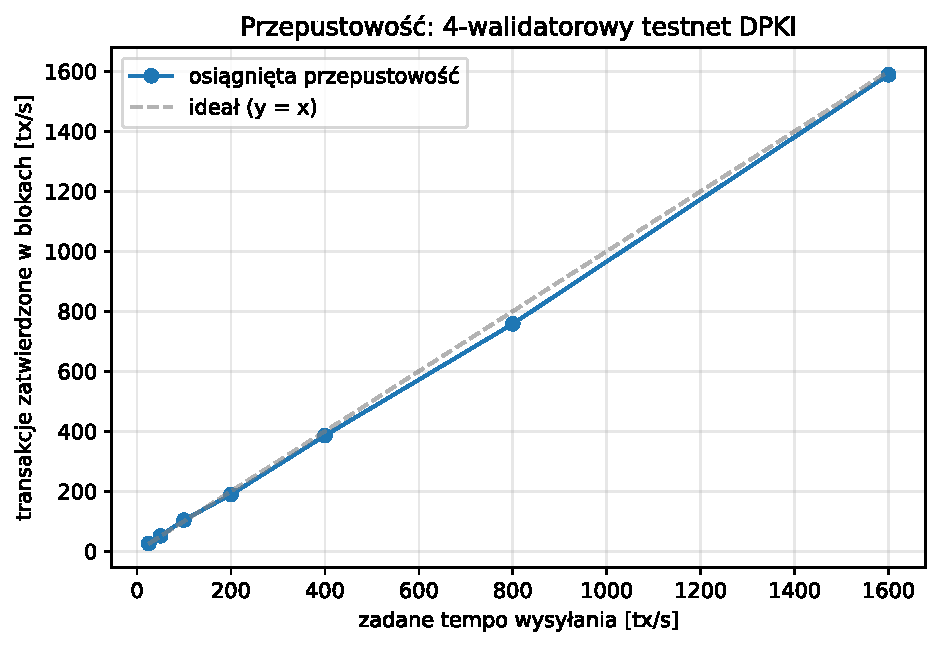
\includegraphics[width=0.85\textwidth]{chart-throughput}
    \caption{Przepustowość osiągnięta w funkcji zadanego tempa obciążenia; linia przerywana oznacza idealną zależność liniową.}
    \label{fig:throughput}
\end{figure}

Najważniejszą obserwacją jest liniowe skalowanie przepustowości w całym zbadanym zakresie - aż do 1588~tx/s przy zadanym tempie 1600~tx/s nie zaobserwowano nasycenia, a wszystkie wysłane transakcje zostały zatwierdzone bez ani jednego odrzucenia. System absorbuje wzrost obciążenia, proporcjonalnie zwiększając liczbę transakcji w bloku (od 31 przy 25~tx/s do niemal dwóch tysięcy przy 1600~tx/s), zamiast wydłużać kolejkę oczekujących. Pierwszego ograniczenia należałoby się spodziewać dopiero powyżej zbadanego zakresu, przy dłuższych falach obciążenia przekraczających domyślną pojemność mempoola. Dla osadzenia tej liczby w kontekście zastosowania: 1588~tx/s odpowiada około 137~milionom operacji na dobę, a więc wartości o rzędy wielkości przewyższającej globalne tempo wystawiania certyfikatów TLS (rzędu kilku milionów dziennie dla największego urzędu). Przepustowość prototypu nie jest zatem czynnikiem ograniczającym dla rozważanego zastosowania.

\subsection{Opóźnienie zatwierdzenia}
\label{subsec:opoznienie}

Opóźnienie zatwierdzenia - czas od wysłania transakcji do jej włączenia w sfinalizowany blok - zmierzono, wysyłając sto transakcji pojedynczo, z przerwą wystarczającą, by każda trafiała w nieskorelowaną fazę interwału bloku. Rozkład wyników podsumowuje tabela~\ref{tab:latencja}, a jego histogram - rysunek~\ref{fig:latency}.

\begin{table}[htbp]
    \centering
    \caption{Statystyki opóźnienia zatwierdzenia transakcji ($n = 100$)}
    \label{tab:latencja}
    \begin{tabular}{l r}
        \hline
        \textbf{Metryka} & \textbf{Wartość [ms]} \\
        \hline
        średnia        & 825 \\
        mediana (p50)  & 813 \\
        percentyl 95 (p95) & 920 \\
        percentyl 99 (p99) & 950 \\
        minimum / maksimum & 784 / 1024 \\
        \hline
    \end{tabular}
\end{table}

\begin{figure}[htbp]
    \centering
    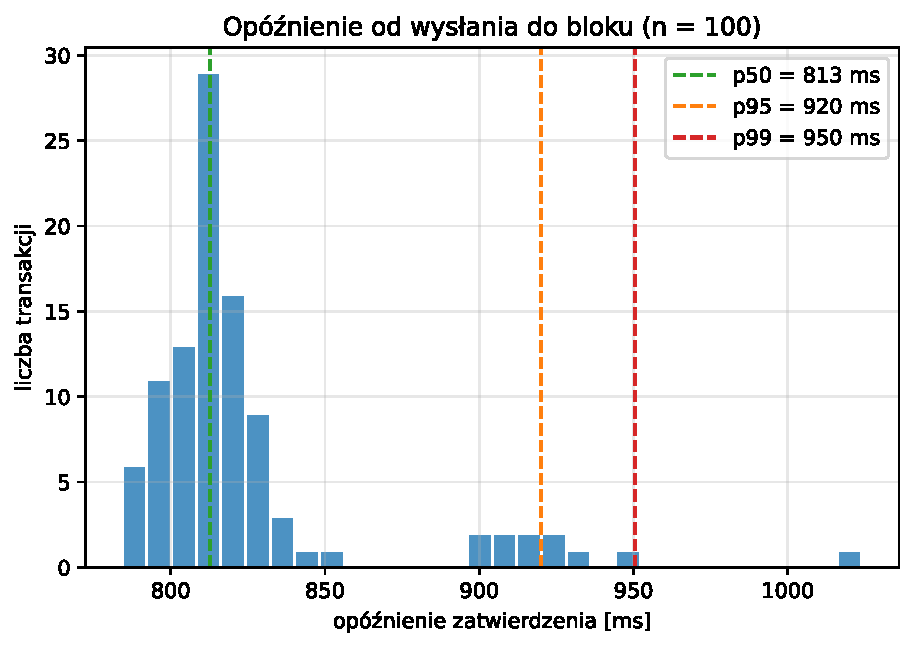
\includegraphics[width=0.85\textwidth]{chart-latency}
    \caption{Histogram opóźnienia zatwierdzenia transakcji wraz z zaznaczonymi percentylami.}
    \label{fig:latency}
\end{figure}

Opóźnienie jest zdominowane przez interwał bloku: transakcja oczekuje średnio około połowy interwału na umieszczenie w propozycji, po czym dochodzi czas rund konsensusu. Mediana 813~ms i niewielki rozrzut między percentylami (różnica p99 i p50 wynosi około 140~ms) świadczą o przewidywalności systemu - opóźnienie jest stabilne, bez długiego ogona. Z punktu widzenia zastosowania kluczowy jest wniosek, że zarówno wystawienie wiązania, jak i jego unieważnienie finalizują się deterministycznie w czasie rzędu jednej sekundy. Stanowi to fundamentalną różnicę względem propagacji unieważnień w klasycznej PKI, liczonej w godzinach lub dniach (sekcja~\ref{sec:crl-ocsp}).

\section{Koszty operacyjne (rozmiar stanu, czas finalizacji)}
\label{sec:koszty}

\subsection{Wzrost stanu}
\label{subsec:wzrost-stanu}

Tempo wzrostu stanu zbadano, wstawiając do drzewa Merkle domeny partiami po dziesięć tysięcy i mierząc po każdej partii rozmiar magazynu oraz średni czas wstawienia. Wyniki przedstawia tabela~\ref{tab:stan}, a zależność rozmiaru stanu od liczby domen - rysunek~\ref{fig:state}.

\begin{table}[htbp]
    \centering
    \caption{Wzrost rozmiaru stanu i czas wstawienia w funkcji liczby domen}
    \label{tab:stan}
    \begin{tabular}{r r r r}
        \hline
        \textbf{Domeny} & \textbf{Magazyn [MB]} & \textbf{Bajtów/domenę} & \textbf{Czas wstawienia [µs]} \\
        \hline
        10\,000  & 156    & $\approx$16\,300 & $\approx$190 \\
        50\,000  & 776    & $\approx$16\,300 & $\approx$180 \\
        100\,000 & 1\,546 & $\approx$16\,200 & $\approx$185 \\
        \hline
    \end{tabular}
\end{table}

\begin{figure}[htbp]
    \centering
    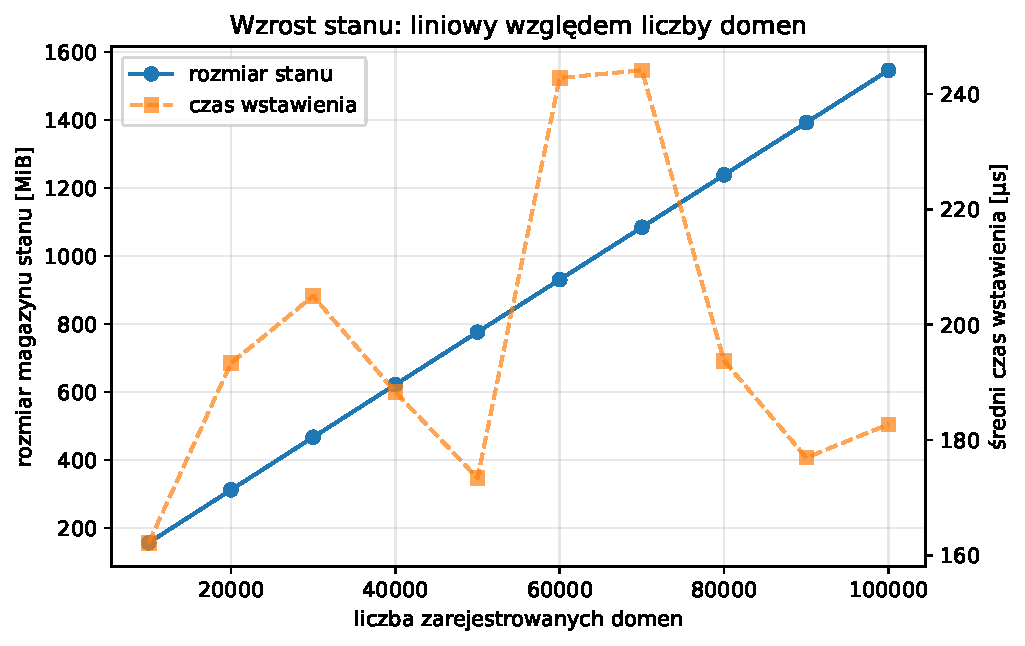
\includegraphics[width=0.85\textwidth]{chart-state-growth}
    \caption{Rozmiar magazynu stanu w funkcji liczby zarejestrowanych domen - zależność liniowa.}
    \label{fig:state}
\end{figure}

Rozmiar stanu rośnie liniowo z liczbą domen, a czas wstawienia pozostaje stały (rzędu 185~µs), niezależny od liczby już zapisanych domen - odzwierciedla to koszt aktualizacji jednej ścieżki w drzewie o stałej głębokości 256. Stały narzut na domenę wymaga jednak uczciwego komentarza, gdyż wartość około 16~kilobajtów znacznie przewyższa rozmiar samego certyfikatu (rzędu 150~bajtów). Różnica nie wynika z rozmiaru danych użytkowych, lecz ze sposobu przechowywania drzewa: w przyjętej, prostej reprezentacji magazyn utrzymuje każdy z węzłów wewnętrznych ścieżki od liścia do korzenia jako osobny wpis. Jest to świadomie zaakceptowany koszt prototypu - produkcyjne implementacje rzadkiego drzewa Merkle stosują kompresję ścieżek (węzły rozszerzające, jak w drzewach Jellyfish Merkle Tree czy Ethereum Merkle Patricia Trie), co redukuje stałą o jeden do dwóch rzędów wielkości, nie zmieniając asymptotycznej złożoności liniowej. Optymalizację tę wskazano jako kierunek dalszych prac (rozdział~\ref{ch:podsumowanie}).

\subsection{Rozmiar i weryfikacja dowodów}
\label{subsec:dowody}

Koszt po stronie strony ufającej wyznacza rozmiar dowodu Merkle oraz czas jego weryfikacji. Zbadano je, próbkując po dwieście losowych dowodów dla trzech rozmiarów drzewa; wyniki zestawia tabela~\ref{tab:dowody}, a zależność rozmiaru dowodu od liczby domen - rysunek~\ref{fig:proof}.

\begin{table}[htbp]
    \centering
    \caption{Rozmiar dowodu i czas weryfikacji w funkcji liczby domen}
    \label{tab:dowody}
    \begin{tabular}{r r r r}
        \hline
        \textbf{Domeny} & \textbf{Dowód włączenia [B]} & \textbf{Dowód nieobecności [B]} & \textbf{Weryfikacja [µs]} \\
        \hline
        1\,000   & 466 & 392 & 27,5 \\
        10\,000  & 572 & 492 & 27,8 \\
        100\,000 & 677 & 605 & 28,0 \\
        \hline
    \end{tabular}
\end{table}

\begin{figure}[htbp]
    \centering
    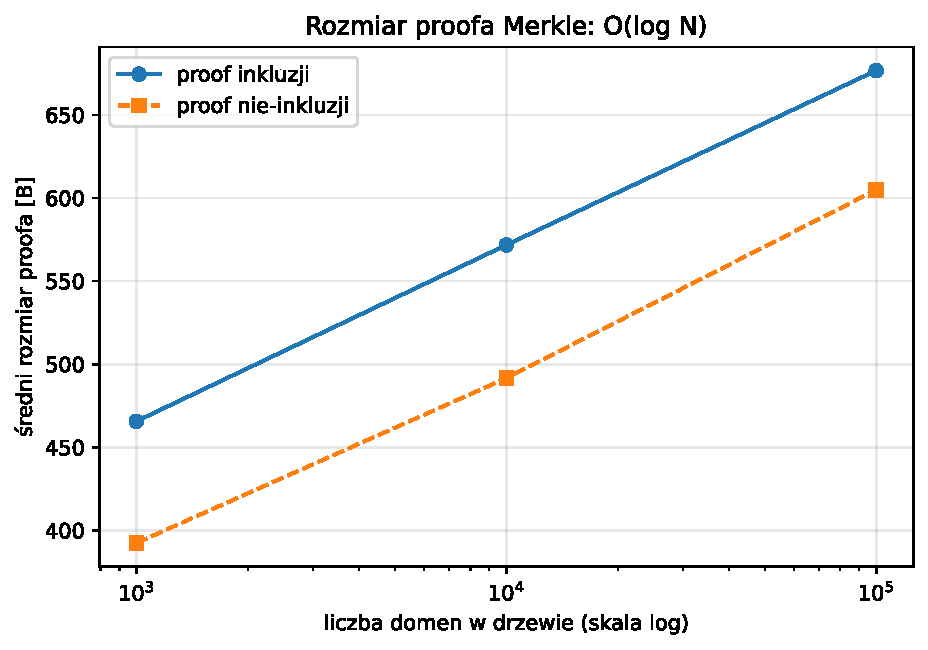
\includegraphics[width=0.85\textwidth]{chart-proof-size}
    \caption{Średni rozmiar dowodu włączenia i nieobecności w funkcji liczby domen (oś pozioma w skali logarytmicznej).}
    \label{fig:proof}
\end{figure}

Rozmiar dowodu rośnie logarytmicznie z liczbą domen - co potwierdza skuteczność kompresji mapą bitową opisanej w sekcji~\ref{subsec:implementacja-merkle} - pozostając w całym zbadanym zakresie poniżej 700~bajtów, podczas gdy czas weryfikacji utrzymuje się na stałym poziomie około 28~mikrosekund. Ekstrapolacja zależności logarytmicznej wskazuje, że nawet dla miliarda domen dowód liczyłby około trzydziestu skrótów rodzeństwa, czyli niewiele ponad kilobajt - wciąż mniej niż typowy łańcuch certyfikatów X.509 (rzędu od dwóch do sześciu kilobajtów). Co istotne, dowód nieobecności ma rozmiar i koszt weryfikacji porównywalny z dowodem włączenia, dzięki czemu weryfikowalna odpowiedź ,,domena nie jest zarejestrowana'' - niedostępna w klasycznej PKI - nie wiąże się z dodatkowym narzutem.

\section{Dyskusja wyników}
\label{sec:dyskusja}

\subsection{Porównanie z klasyczną PKI}
\label{subsec:porownanie-wydajnosc}

Zmierzone charakterystyki pozwalają uzupełnić jakościowe porównanie z rozdziału~\ref{ch:analiza-bezpieczenstwa} o wymiar ilościowy. Zestawienie przedstawia tabela~\ref{tab:porownanie-wyd}.

\begin{table}[htbp]
    \centering
    \caption{Ilościowe porównanie kosztów operacji klasycznej PKI i zaproponowanego systemu}
    \label{tab:porownanie-wyd}
    \begin{tabular}{p{0.28\textwidth} p{0.32\textwidth} p{0.32\textwidth}}
        \hline
        \textbf{Kryterium} & \textbf{Klasyczna PKI (X.509 + CA)} & \textbf{DPKI (zmierzono)} \\
        \hline
        Czas wystawienia & minuty--dni (proces CA) & p50 = 0,81~s (następny blok) \\
        Propagacja unieważnienia & godziny--dni (CRL/OCSP, \emph{soft-fail}) & p50 = 0,81~s, trwała \\
        Rozmiar dowodu ważności & łańcuch certyfikatów 2--6~kB oraz odpowiedź OCSP & dowód 0,5--0,7~kB, weryfikowalny offline \\
        Czas weryfikacji & rząd milisekund (łańcuch podpisów) & 28~µs (dowód) plus weryfikacja podpisu \\
        Dowód nieistnienia & niedostępny & dowód nieobecności rzędu 0,5~kB \\
        Infrastruktura weryfikatora & dostęp do OCSP/CRL w trybie online & zaufany skrót stanu i obliczenie lokalne \\
        \hline
    \end{tabular}
\end{table}

Najwyraźniejsza przewaga ilościowa dotyczy unieważnień: mechanizm propagujący się w czasie jednej sekundy i dający trwały, dowodliwy skutek zastępuje infrastrukturę CRL/OCSP o propagacji liczonej w godzinach i obarczonej praktyką \emph{soft-fail}, która w klasycznym modelu osłabia samą skuteczność unieważnienia (sekcja~\ref{sec:crl-ocsp}). Drugą zauważalną różnicą jest charakter dowodu ważności - zwięzły, weryfikowalny w trybie offline dowód Merkle nie wymaga od weryfikującego łączności z infrastrukturą statusu w momencie weryfikacji, w odróżnieniu od odpytywania respondera OCSP.

\subsection{Skalowalność i jej ograniczenia}
\label{subsec:skalowalnosc}

Zmierzone zależności pozwalają wskazać granice skalowalności systemu. Po stronie konsensusu zasadniczym ograniczeniem jest komunikacja o złożoności kwadratowej względem liczby walidatorów, właściwa protokołom BFT (sekcja~\ref{subsec:bft-tendermint}); wyznacza ona praktyczny pułap rzędu setek walidatorów i sprawia, że dodawanie walidatorów zwiększa odporność, lecz nie przepustowość. Po stronie stanu wzrost jest liniowy i nieograniczony z góry, a istotnym czynnikiem jest tu trwałość unieważnień (sekcja~\ref{subsec:uniewaznienie}): unieważnione wpisy muszą pozostać w stanie, co wyklucza ich usuwanie. Po stronie klienta koszt weryfikacji pozostaje praktycznie stały - logarytmiczny rozmiar dowodu czyni klienta lekkim niezależnie od rozmiaru rejestru. Wreszcie, koszt odzyskiwania stanu przez ponowne odtworzenie historii (sekcja~\ref{subsec:zarzadzanie-stanem}) rośnie liniowo z długością łańcucha - akceptowalny dla prototypu, lecz we wdrożeniu produkcyjnym wymagałby trwałego magazynu stanu. Kierunki łagodzenia tych ograniczeń - kompresja ścieżek drzewa, podział rejestru oraz pełny lekki klient - omówiono w rozdziale~\ref{ch:podsumowanie}.

\subsection{Wnioski}
\label{subsec:wnioski-eksperymenty}

Przeprowadzone pomiary prowadzą do spójnego wniosku: zaproponowany system osiąga przepustowość i opóźnienie o rzędy wielkości lepsze niż procesy klasycznej PKI tam, gdzie ma to największe znaczenie dla bezpieczeństwa - w propagacji unieważnień - przy koszcie w postaci stałego narzutu pamięciowego na domenę oraz ograniczenia skali zbioru walidatorów. Koszt ten jest bezpośrednią konsekwencją zamiany zaufanej trzeciej strony na replikowaną maszynę stanów: bezpieczeństwo i transparentność uzyskuje się tu przez redundancję i jawność, nie zaś przez zaufanie do pojedynczego podmiotu. Wartości bezwzględne, uzyskane w środowisku jednomaszynowym, należy traktować jako orientacyjne, jednak zaobserwowane relacje - liniowy wzrost stanu, logarytmiczny rozmiar dowodu, stały koszt weryfikacji - są niezależne od środowiska i potwierdzają praktyczną wykonalność oraz skalowalność przyjętego podejścia w zakresie istotnym dla zastosowania.

%!TEX root = ../main.tex
\chapter{Podsumowanie}
\label{ch:podsumowanie}

\section{Realizacja celów pracy}
\label{sec:realizacja-celow}

Głównym celem pracy było zaprojektowanie, implementacja oraz analiza bezpieczeństwa zdecentralizowanej infrastruktury klucza publicznego opartej na technologii blockchain, stanowiącej alternatywę dla scentralizowanego modelu PKI X.509 w zakresie Web PKI. Cel ten zrealizowano w pełnym zakresie: powstał działający prototyp - rejestr wiązań domena--klucz utrzymywany przez sieć walidatorów z konsensusem BFT (rozdziały~\ref{ch:projekt}--\ref{ch:implementacja}) - który poddano systematycznej analizie bezpieczeństwa (rozdział~\ref{ch:analiza-bezpieczenstwa}) oraz ocenie ilościowej (rozdział~\ref{ch:eksperymenty}). Poniżej odniesiono uzyskane wyniki do tezy głównej oraz czterech tez pomocniczych.

\paragraph{Teza główna.} Teza głosząca, że DPKI oparta na blockchain z konsensusem BFT może stanowić funkcjonalnie kompletną alternatywę dla klasycznego modelu PKI X.509 w zakresie Web PKI, eliminując pojedynczy punkt zaufania w postaci centrów certyfikacji, została potwierdzona. Zaimplementowany system realizuje pełny cykl życia wiązania domena--klucz - rejestrację, rotację, unieważnienie oraz weryfikację z dowodem (sekcja~\ref{sec:protokoly}) - a więc jest funkcjonalnie kompletny w rozważanym zakresie. Pojedynczy punkt zaufania został wyeliminowany: jak wykazano w sekcji~\ref{sec:porownanie-bezpieczenstwa}, kompromitacja mniejszości walidatorów nie narusza integralności rejestru, a osiągnięcie progu dwóch trzecich prowadzi co najwyżej do wstrzymania systemu, nie zaś do wystawienia fałszywego wiązania - w przeciwieństwie do modelu klasycznego, w którym kompromitacja dowolnego z setek urzędów wystarcza do wystawienia fałszywego certyfikatu dla dowolnej domeny.

\paragraph{Teza pomocnicza pierwsza.} Potwierdzono, że zastąpienie hierarchii CA rozproszonym rejestrem eliminuje klasę ataków polegających na kompromitacji pojedynczego urzędu, przy czym część zagrożeń pozostaje aktualna. Analiza bezpieczeństwa (rozdział~\ref{ch:analiza-bezpieczenstwa}) wykazała odporność na nieautoryzowane wystawienie i modyfikację wiązań, lecz zarazem uczciwie wskazała zagrożenia rezydualne (sekcja~\ref{sec:ograniczenia}): kompromitację DNS w oknie rejestracji oraz utratę klucza prywatnego właściciela. Zgodnie z przewidywaniem tezy, zagrożenia te dotyczą bezpieczeństwa klucza właściciela i integralności procesu weryfikacji, a więc wymagają niezależnego adresowania, którego sam rejestr nie zapewnia.

\paragraph{Teza pomocnicza druga.} Potwierdzono, że wprowadzenie warstwy konsensusu i sieci P2P rodzi nowe wektory ataku, których realizacja jest jednak istotnie trudniejsza niż kompromitacja pojedynczego CA. Przeanalizowane ataki na konsensus i warstwę sieciową (sekcje~\ref{subsec:kompromitacja-walidatora}--\ref{subsec:sybil-eclipse}) wymagają bądź kontroli ponad jednej trzeciej mocy głosów walidatorów, bądź aktywnej manipulacji ruchem sieciowym - w obu przypadkach progu nieporównanie wyższego niż kompromitacja jednego z setek urzędów w modelu klasycznym. Empirycznie potwierdzono przy tym, że awaria mniejszości walidatorów nie narusza bezpieczeństwa systemu, a jedynie - po przekroczeniu progu kworum - jego dostępność.

\paragraph{Teza pomocnicza trzecia.} Potwierdzono, że zapis stanu w drzewie Merkle umożliwia protokół wiązania pozbawiony zaufanego pośrednika, z gwarancjami silniejszymi niż CRL/OCSP przy niższym koszcie weryfikującego. Weryfikacja istnienia, ważności i unieważnienia odbywa się przez sprawdzenie dowodu względem skrótu stanu, bez odpytywania scentralizowanej infrastruktury statusu (sekcja~\ref{sec:api}). Pomiary (sekcja~\ref{subsec:dowody}) wykazały, że dowód ma rozmiar poniżej 700~bajtów i weryfikuje się w czasie około 28~mikrosekund - a więc taniej niż łańcuch certyfikatów X.509 wraz z odpowiedzią OCSP - a jego rozmiar rośnie jedynie logarytmicznie z liczbą domen. Co więcej, system dostarcza weryfikowalnego dowodu nieistnienia wiązania, niedostępnego w modelu klasycznym.

\paragraph{Teza pomocnicza czwarta.} Potwierdzono, że wykorzystanie gotowej warstwy konsensusu CometBFT oraz interfejsu ABCI pozwala zaimplementować funkcjonalną DPKI wyłącznie w warstwie aplikacyjnej. Cała logika rejestru zamknęła się w aplikacji ABCI (sekcja~\ref{sec:aplikacja-abci}), bez modyfikowania protokołu konsensusu, sieci P2P czy mechanizmu replikacji bloków - co potwierdza praktyczną wykonalność budowy DPKI z gotowych komponentów i stanowi zarazem odpowiedź na pytanie o praktyczną realizowalność takiego systemu.

\section{Wnioski}
\label{sec:wnioski}

Z przeprowadzonej pracy płynie wniosek nadrzędny: zdecentralizowana infrastruktura klucza publicznego oparta na konsensusie BFT jest praktycznie wykonalna i adresuje zasadniczą, strukturalną słabość klasycznej PKI - istnienie pojedynczego punktu zaufania o nieograniczonym zakresie. Zamiast bezwarunkowego zaufania do każdego z setek urzędów certyfikacji, system opiera zaufanie na założeniu o uczciwości ponad dwóch trzecich znanego zbioru walidatorów, czyniąc kompromitację mniejszości nieszkodliwą, a kompromitację większości - prowadzącą do wstrzymania, nie zaś do fałszerstwa.

Praca pozwala też sformułować wniosek o naturze kosztu tej zmiany. Bezpieczeństwo i transparentność uzyskuje się tu przez redundancję i jawność, a nie przez zaufanie do pojedynczego podmiotu - a ceną jest replikacja stanu na wszystkich walidatorach (stały narzut pamięciowy na domenę, sekcja~\ref{subsec:wzrost-stanu}) oraz ograniczenie skali zbioru walidatorów wynikające ze złożoności komunikacji konsensusu (sekcja~\ref{subsec:skalowalnosc}). Jest to kompromis odmienny niż w modelu klasycznym, lecz - jak wykazały pomiary - mieszczący się w granicach praktycznej użyteczności dla rozważanego zastosowania.

Na poziomie szczegółowym praca uwidoczniła kilka rozstrzygnięć projektowych o znaczeniu wykraczającym poza sam prototyp. Najważniejszym z nich jest rola granicy determinizmu wyznaczonej przez interfejs ABCI: konieczność utrzymania w pełni deterministycznego wykonania w ramach konsensusu wymusiła umieszczenie niedeterministycznej weryfikacji DNS jako bramki przedkonsensusowej (sekcja~\ref{sec:wlasnosc-domeny}), co okazało się rozwiązaniem godzącym wymóg weryfikacji własności domeny z wymogiem powtarzalności stanu, a zarazem umożliwiającym odtwarzanie historii przy odzyskiwaniu po awarii. Drugim jest trwałość unieważnienia, która - choć pozornie jest jedynie szczegółem implementacyjnym - okazała się kluczowa dla odporności na atak ,,od-unieważnienia'' w scenariuszu kompromitacji klucza (sekcja~\ref{subsec:ataki-kryptograficzne}).

Należy przy tym zachować właściwą miarę w ocenie wyników. Prototyp nie jest gotowym do wdrożenia produktem, a przeprowadzone testy bezpieczeństwa dowodzą odporności na konkretne, rozważone ataki, nie zaś bezpieczeństwa systemu w sensie absolutnym (sekcja~\ref{sec:model-zagrozen}). Podobnie pomiary wydajnościowe, uzyskane w środowisku jednomaszynowym, dają wartości orientacyjne; wiarygodne pozostają natomiast zaobserwowane relacje asymptotyczne, niezależne od środowiska.

\section{Kierunki dalszych prac}
\label{sec:dalsze-prace}

Praca otwiera kilka naturalnych kierunków kontynuacji, sygnalizowanych w poprzednich rozdziałach. Wynikają one bądź z ograniczeń prototypu, bądź z możliwości jego rozszerzenia o funkcje istotne dla wdrożenia produkcyjnego.

\begin{itemize}
    \item \textbf{Trwały magazyn stanu} - zastąpienie magazynu w pamięci operacyjnej wbudowaną bazą klucz--wartość, za istniejącą już abstrakcją interfejsu magazynu (sekcja~\ref{subsec:zarzadzanie-stanem}). Wyeliminowałoby to konieczność odtwarzania całej historii po restarcie węzła, której koszt rośnie liniowo z długością łańcucha.
    \item \textbf{Kompresja ścieżek drzewa} - zastosowanie węzłów rozszerzających, na wzór drzew stosowanych w systemach produkcyjnych, w celu zmniejszenia stałego narzutu pamięciowego na domenę o jeden do dwóch rzędów wielkości (sekcja~\ref{subsec:wzrost-stanu}), bez zmiany liniowej złożoności asymptotycznej.
    \item \textbf{Pełny lekki klient} - rozszerzenie klienta o weryfikację podpisów walidatorów nad nagłówkami bloków, co domknęłoby lukę w scenariuszu eclipse klienta (sekcja~\ref{subsec:sybil-eclipse}) i zapewniło pełną minimalizację zaufania także w warunkach izolacji sieciowej.
    \item \textbf{Skalowanie poziome} - podział rejestru (np.\ według domen najwyższego poziomu) w celu obejścia ograniczenia skali wynikającego z kwadratowej złożoności komunikacji pojedynczego zbioru walidatorów (sekcja~\ref{subsec:skalowalnosc}).
    \item \textbf{Wieloalgorytmiczność} - rozszerzenie obsługi o dodatkowe algorytmy podpisu poza Ed25519, na które schemat danych już pozostawia miejsce (sekcja~\ref{subsec:reprezentacja-cert}), oraz rozważenie algorytmów odpornych na komputery kwantowe.
    \item \textbf{Integracja z istniejącym ekosystemem} - zbadanie ścieżek współdziałania z obecną Web PKI, w szczególności sposobów wykorzystania zweryfikowanego wiązania przez klientów TLS bez konieczności zmiany całego stosu zaufania naraz.
\end{itemize}

Realizacja powyższych kierunków przybliżyłaby prototyp do rozwiązania zdatnego do wdrożenia, nie zmieniając jednak zasadniczego wyniku niniejszej pracy: wykazania, że zdecentralizowana infrastruktura klucza publicznego oparta na konsensusie BFT jest praktycznie wykonalna i stanowi wiarygodną odpowiedź na strukturalne słabości scentralizowanego modelu zaufania.


\printbibliography[heading=bibintoc]

\listoffigures
\listoftables
\lstlistoflistings

\end{document}